% CABECERA
% BEGIN_FOLD
%%%%%%%%%%%%%%
% Fichero: uclmTFGesi.tex
% Autor: Jesús Salido Tercero (https://www.esi.uclm.es/www/jsalido)
% Fecha (creación): Febrero 2010 
% Rev. : Febrero 2021
% Descripción: Plantilla para memoria de TFG 
% (Escuela Sup. de Informática, UCLM). Creada para el curso 
% “LaTeX esencial para preparación de TFG, Tesis y otros documentos 
% académicos” (Esc. Sup. Informática-UCLM)
%
%### Compilación 
%
% Esta plantilla ha sido preparada para compilarse con `pdflatex`, `biblatex` 
% (bibliografía con `biber`) y `makeindex` (sólo si se incluye índice 
% temático).
%
% Para su compilación se aconseja utilizar `latexmk` (requiere para su 
% ejecución de un intérprete perl:
%
%> \$> latexmk -gg -pdflatex -bibtex-cond1 -silent -auxdir=build -outdir=build uclmTFGesi.tex
%
% Para la automatización del trabajo con esta plantilla es recomendable el 
% empleo de IDE dedicados como [TeXstudio](https://www.texstudio.org/).
%
% Una versión revisada de esta plantilla está disponible en overleaf.
% Puede crearse un proyecto propio para escribir un TFG directamente en 
% overleaf, o bien descargarla como un archivo .zip para su utilización en 
% modo local.
%
% Si deseas acceder a la versión de desarrollo puedes encontrarla en GitHub:
%	https://github.com/JesusSalido/TFG_ESI_UCLM
%%%%%%%%%%%%%%
% END_FOLD


% -------------------------
%
% PREÁMBULO
% BEGIN_FOLD
% -------------------------
\documentclass[ 		% Clase del documento
	11pt,				% Tamaño de letra
	a4paper,			% Tamaño de papel
	twoside,			% Impresión a doble cara
	openright,			% La apertura de cap. a la dcha.
%	draft       		% Versión borrador (sin figuras)
	final       		% Versión final
]{book}

%--- Codificación de entrada (mejora respecto a inputenc)
\usepackage[utf8]{inputenx} 
\usepackage[
    english,     % Se emplea porque el resumen siempre en inglés
    spanish,     % Se emplea para resumen en español
    es-tabla,    % Si idioma pral. español
    es-noindentfirst
]{babel} % Internacionalización


%--- Geometría de las páginas del documento
\usepackage[			% Márgenes del documento
	top=2.5cm,			% Margen superior
	bottom=2.5cm,		% Margen inferior
	inner=3.5cm,		% Margen al interior
	outer=2cm			% Margen al exterior
]{geometry}

%--- Tipografía
\usepackage{amsmath,amssymb,amsfonts} % Para ecs.

%--- Si no se emplea ningún paquete de tipografía se empleará Computern Modern.
%--- Tipografía 
%--- (Opción: Latin Modern)
%\usepackage{lmodern} % Latin Modern. Empleada cuando se desea una tipografía genuina de LaTeX sucesora de Computer Modern.
%--- (Opción: Libertine)
\usepackage[tt=false]{libertine} % Libertine con Old-Style Figures [osf]
\usepackage[libertine]{newtxmath} % Times
%--- (Opción: Palatino)
%\usepackage{newpxtext} % Palatino: La opción osf proporciona números en old style.
%\usepackage{newpxmath}	% Palatino
%--- (Opción: Fourier)
%\usepackage{fourier} % Utopía
%---

%--- (Opción excepcional)
% Si es preciso cambio de tipo de familia de tipografía por defecto a Sans-Serif
% Aunque es una opción extraña es la preferida en algunos centros docentes (ADE-UCLM).
% Con esta elección es más conveniente una tipografía tipo Helvética/Arial (no Libertine)
%\usepackage{helvet}
%\renewcommand{\familydefault}{\sfdefault}
%---

\usepackage{textcomp,marvosym,pifont} % OPT.: Generación de símbolos 
%especiales
\usepackage{ccicons} % OPT.: Iconos de licencia Creative Commons
\usepackage[T1]{fontenc}% Codificación de salida    

%--- Paquete con personalización local para el TFG (ESI-UCLM)
% EDITAR: Si es preciso que la memoria emplee "english" como idioma 
% principal, prefijos de género y ubicación en número de página al pie.
% Con la opción "english" el resto de opciones son irrelevantes.
% Los prefijos de género permiten un tratamiento adecuado en portadas
% automáticas.
%
% Opciones del paquete: (por defecto) Memoria en español y prefijos masculinos.
%	spanish: idioma pral. español (valor por defecto).
%   english: idioma pral. inglés.
%	autora,tutora,cotutora: indica el género de intervinientes (masculino por defecto) 	
%	pageonfooter: Número de página en el pie y centrado como ADE-UCLM (por defecto en cabeceras)
% -------------------------
% COMANDOS OPCIONALES PROPORCIONADOS:
% OP-Opcional
% RE-Recomendado
%
% Comandos de generación automática de portadas
% \portadaTFG, \portadaTFG*{ficheroPDF}: Página de portada
% \portillaTFG, \portadillaTFG*{ficheroPDF}: Página de contraportada
% \tribunalTFG, \tribunalTFG*{ficheroPDF}: Página de tribunal
% \dedicado{texto}: Dedicatoria
% \creditos{texto}{fichero gráfico de licencia}
%
% Comandos para definir variables con los datos del documento.
%
% OP-\nodivide[penalty]			: Penaliza la división de palabras. Máx. 
%								: (n=10000) sin arg.
% OP-\nowidowandorphan[penalty] : Penaliza las viudas y huérfanas. (sólo si necesario)
% OP-\nodividenotes[penalty]	: Penaliza la división de notas al pié entre págs.	(sólo si necesario)	
% OP-\savepagecnt				: Salva en un contador interno el nº de pág. actual
% OP-\contpagination			: Recupera el valor de pág. previamente salvado en el cont. interno.
% OP-\tecla{texto}				: Genera un borde de tecla en torno al 
%texto		
% -------------------------
%\usepackage{uclmTFGesi}
\usepackage[tutora,cotutora]{uclmTFGesi}
%\usepackage[pageonfooter]{uclmTFGesi}



%--- Bibliografía: Biblatex con biber.
% Permite cambiar los estilos de citación y ordenación de la bibliografía
\usepackage[%
	backend=biber,
	% Estilos: numeric, numeric-comp, alphabetic, authoryear, authoryear-comp
	% Otros: apa, chicago, ieee, mla-new, iso-numeric, iso-authoryear
	% Estilos tradicionales BibTeX: trad-plain, trad-unsrt, trad-alpha y trad-abbrv
%	bibstyle=apa, % Estilo APA
	bibstyle=ieee,
	% Citación: numeric, numeric-comp, numeric-verb, 
	%           authoryear, authoryear-comp,...
	%           otros aplicados con estilo gral.: ieee,apa,aml,chem-acs,iso-numeric,iso-authoryear
	citestyle=numeric-comp,
	sortcites, % Ordenación de citas múltiples cuando son numéricas
	maxbibnames=3, % Máximo número listado de autores en la bibliografía
	minbibnames=1, % Mínimo número de autores cuando se abrevia la lista de autores
	% Descomentar las opciones siguientes para bibliografía multilingüe
	autolang=other, % Requerido para opción multilingüe
	language=auto,   % Requerido para opción multilingüe
	sorting=nyt%
					% Para cambiar criterio de ordenación de las referencias.
 					% =nty (name-title-year), nyt (name-year-title), nyvt (name-year-volume-title), 
					% =anyt (alphabetic-name-year-title), anyvt (alphabetic-name-year-volume-title), 
					% =ynt (year-name-title), ydnt (yeardescendent-name-title), 
					% =none (por orden de citación, como en ETSII-UCLM).			
]{biblatex}

% Línea añadida para eliminar el idioma de la fuente bibliográfica.
\AtEveryBibitem{\clearfield{note} \clearlist{language}}


% OPT: No comentar si es necesario suprimir el sangrado de párrafos.
%\setlength{\parindent}{0pt} % Elimina sangrado de párrafos

\addbibresource{biblioTFG.bib} 	% Fichero de bibliografía.

\DeclareGraphicsExtensions{.pdf,.png,.jpg,.jpeg} % Precedencia de extensiones
\graphicspath{{./figs/}}% Path de búsqueda de ficheros gráficos

\usepackage{makeidx} % Indice temático

% END_FOLD
% EDITAR: Descomentar si se desea índice temático
%\makeindex           % OPT.: Procesamiento de índice temático
% -------------------------
% -------------------------
% -------------------------

% Mis paquetes/imports añadidos
\usepackage{xcolor} % Colores
\definecolor{green}{RGB}{34, 139, 34}
\definecolor{red}{RGB}{255, 40, 40}
\definecolor{blue}{RGB}{64, 64, 255}
\definecolor{orange}{RGB}{255, 128, 0}


% DATOS del documento
% EDITAR: Datos del documento. 
% Los elementos opcionales pueden dejarse, eliminarse o comentarse. No se deben dejar vacíos porque provoca errores.
% BEGIN_FOLD
% -------------------------
% -------------------------
% -------------------------
% DATOS DEL DOCUMENTO 
% Definición de variables empleadas en el documento por lo que no son
% traducidos. Cuando algún campo puede tener varias líneas aparecen dos
% campos señalados como <campo>Primera y <campo>Segunda. Si no se desea 
% emplear los campos opcionales (OPT.) estos deben comentarse.
% -------------------------
\tituloPrimera{Diseño e Implementación de un SDK Android para Facilitar la Interacción de Aplicaciones Móvil con una Blockchain} % 1ª Línea
% \tituloSegunda{Curso de {\LaTeX{}} esencial} % OPT.: Para títulos largos.
\titulo{SDK Android con interacción con Blockchain} % Título corto (mostrado en pág. de créditos)
\autor{Jorge Sol Gonzalez}
\email{jorge.sol.gonzalez@alumnos.upm.es}					
\tutor{Francisco javier Soriano Camino} % Sólo nombre, el prefijo añadido automát.
% \cotutor{<co-tutor(a) (nombre apellidos)>}	% OPT.: Cotutor(a)
\instEdu{UNIVERSIDAD POLITÉCNICA DE MADRID}

% Fichero con escudo de la institución
% Logo de la ESI que prefieras (la normativa no especifica obligatoriedad).
%\escudo{esi} 					% Logo ESI (gris uniforme)							
%\escudo{esi_black} 			% Logo ESI (negro)						
%\escudo{esi_color}				% Logo ESI (dos tintas)						
\escudo{IngInformatica_color}	% Nucleo de ferrita	(color)
%\escudo{IngInformatica_bw} 	% Nucleo de ferrita	(en escala de grises)					

\centroEdu{ESCUELA TÉCNICA SUPERIOR DE INGENIEROS INFORMÁTICOS}
\deptoEduPrimera{Departamento de Lenguajes y Sistemas} % 1ª Línea(EN: Department of ...)
% \deptoEduSegunda{<Segunda línea Depto. Director>} % OPT.: Para nombres largos.
\titulacion{GRADO EN INGENIERÍA INFORMÁTICA} % (EN: BACHELOR IN COMPUTING ENGINEERING)
% \especialidad{<Tecnología Específica>} % OPT.: Especialidad - Intensificación
% (EN: Specialization in ...)
\tipoDoc{TRABAJO FIN DE GRADO} % (EN: BACHELOR DISSERTATION)

% Si las fechas se desean en inglés hay que ponerla explícita.
\fechaDef{junio, 2021} 			% Fecha de defensa
\mesDef{junio}        			% Mes de defensa
\yearDef{2021}        			% Año de defensa
\lugarDef{Madrid}			% Lugar de defensa


% --- Metadatos (propiedades) para el documento PDF
\hypersetup{% OPT.
	pdftitle={Diseño e Implementación de un SDK Android para Facilitar la Interacción de Aplicaciones Móvil con una Blockchain}, % Título
	pdfauthor={Jorge Sol Gonzalez}, % Autor
	pdfsubject={TFG},  % Tema
	pdftoolbar=true, % Muestra la toolbar de Acrobat
	pdfmenubar=true	 % Muestra la menubar de Acrobat
}
% -------------------------
% -------------------------
% -------------------------
% END_FOLD



% -------------------------
% -------------------------
% -------------------------
% -------------------------
%
% CUERPO del documento
%
% -------------------------
\begin{document}
%--- PORTADAS + FRONTMATTER
\frontmatter
% Cambia la numeración de páginas a números romanos y las secciones no están 
%numeradas aunque si aparecen en el índice de contenidos.
\pagestyle{empty}  % Páginas sin cabecera ni pies

\includecomment{portadas} % Cambiar por exclude para evitar compilar portadas
%\excludecomment{portadas} % Cambiar por exclude para evitar compilar portadas
\begin{portadas}
% -------------------------
% -------------------------
% -------------------------
%
% PORTADAS: 
%
% Los comandos \portadaTFG y \portadilla generan dos portadas con LaTeX 
% teniendo en cuenta los datos sobre el documento aportados en el preámbulo.
% Si se desea incluir una portada generada externamente en PDF se emplea la
% versión del comando con estrella indicando el fichero.
%
% -------------------------





%---
% \portadaTFG		% Portada pral.
%\portadaTFG*{./figs/portadaETSII} % Portada generada externamente en PDF
% También en versión con estrella para indicar fichero PDF
% Comentar si no se desea incluir
%---






%---
\portadillaTFG	% Portada interior (con tutor(a) y co-tutor(a) si existe).
% También en versión con estrella para indicar fichero PDF
% Comentar si no se desea incluir
%---





%---
% OPT.: CRÉDITOS (aunque no es obligatorio es recomendable).
% % -------------------------
%
% CRÉDITOS
%
% -------------------------
% EDITAR: El autor puede elegir el tipo de licencia que desee para distribuir su TFG que puede variar con respecto a la de este documento en el que si permitimos obra derivada para que no surjan dudas sobre la reutilización del material.
% Este comando permite una gran flexibilidad y la ventaja de no depender de paquetes externos.
% Esta es una página reservada para señalar información relativa a los derechos de autor y la licencia de distribución y uso del documento. Esta página debería ser aprovechada también para informar de cualquier tipo de cesión de los derechos anteriormente citados. El autor del TFG debe tener presente que el incumplimiento de la legislación vigente en materia de protección de la propiedad intelectual es de su exclusiva responsabilidad independientemente de la cesión de derechos que este haya convenido para su obra ya que no son objeto de cesión aquellos derechos de los que no se es poseedor.

\creditos{Este documento se distribuye con licencia CC BY-NC-SA 4.0. El texto completo de la licencia puede obtenerse en \url{https://creativecommons.org/licenses/by-nc-sa/4.0/}.

La copia y distribución de esta obra está permitida en todo el mundo, sin regalías y por cualquier medio, siempre que esta nota sea preservada. Se concede permiso para copiar y distribuir traducciones de este libro desde el español original a otro idioma, siempre que la traducción sea aprobada por el autor del libro y tanto el aviso de copyright como esta nota de permiso, sean preservados en todas las copias.

% NOTA: Deja esta nota de atribución al uso de la plantilla LaTeX.
Este texto ha sido preparado con la plantilla \LaTeX{} de TFG para la UCLM publicada por \href{https://www.esi.uclm.es/www/jsalido}{Jesús Salido} en GitHub\footnote{\url{https://github.com/JesusSalido/TFG_ESI_UCLM}} y Overleaf \footnote{\url{https://www.overleaf.com/latex/templates/plantilla-de-tfg-escuela-superior-de-informatica-uclm/phjgscmfqtsw}} como parte del curso \href{http://visilab.etsii.uclm.es/?page_id=1468}{\emph{<<\LaTeX{} esencial para preparación de TFG, Tesis y otros documentos académicos>>}} impartido en la Escuela Superior de Informática de la Universidad de Castilla-La Mancha.}{by-nc-sa}


% NOTA: Para citar este documento puede emplear el registro siguiente:
%@www{salidoTFG,
%  author       = {Jesús Salido},
%  title        = {Plantilla guía de TFG para la ESI-UCLM},
%  year         = {2019},
%  editor       = {GitHub},
%  organization = {Universidad de Castilla-La Mancha},
%  url          = {https://github.com/JesusSalido/TFG_ESI_UCLM},
%}


%---



%---




%---
% \tribunalTFG % Página para calificaciones del tribunal
% También en versión con estrella para indicar fichero PDF
%---





%---
% OPT.: DEDICATORIA (1 pág. máximo) comentar si no se desea incluir.
% Aunque opcional, no se debería perder la oportunidad de poder 
% dedicar el trabajo a alguien MUY especial.
% EDITAR: Dedicatoria.
\dedicado{A mis amigos y familia, \\ % A alguien muy especial
por aguantarme todos los días.} % Como mucho dos líneas (no confundir con los agradecimientos).
%---
%
% FIN PORTADAS: 
% |
% |
% -> ----------------------
\end{portadas}

% Puedes comentar los apartados que no deseas compilar
\pagestyle{plain}

\selectlanguage{spanish}
\cleardoublepage
\phantomsection
\addcontentsline{toc}{chapter}{Resumen}

\begin{abstract}
  % Resumen Introducción y Estado del Arte
  Durante los últimos dos años se ha tenido la oportunidad de trabajar en la Cátedra Inetum investigando y estudiando todo lo relacionado a la tecnología blockchain. Dentro de esta cátedra, surgió un proyecto llamado ``Estublock'' con el cual se pretende resolver un problema más común de lo deseado. Es habitual que todos los años algún alumno acuse a un profesor de perder su exámen. La universidad se encuentra ante la decisión de creer al alumno que promete haber asistido al exámen, o el profesor que promete no tener dicho exámen. El problema radica, en que no hay una forma común y fiable de validar la asistencia a exámenes (y otros eventos). Para solucionar este problema se quiere usar blockchain, esta tecnología viene a ser como una base de datos distribuida que guarda transacciones. Transacciones monetarias, transacciones con información o datos como el nombre de una persona, un billete de avión, un entrada de cine\dots La red blockchain elegida para el trabajo es la red de Ethereum, gracias a que tiene la posibilidad de ejecutar Smart Contracts en ella. Los smart contracts son básicamente código que se ejecuta de manera automática ante una llamada a una de sus funciones. En el presente existen varios proyectos que aprovechan la red de Ethereum, como \emph{Guts, LifeID y Voatz}. Para desarrollar ``Estublock'' se ha utilizado Android, uno de los sistemas operativos más utilizados en el presente y para facilitar la comunicación con la base de datos y algunos procesos de la comunicación con la red blockchain, se ha desarrollado una API RESTful. \\

  % Resumen Desarrollo
  El desarrollo de la aplicación y del SDK han supuesto un gran reto. Se trata de un campo que nunca antes se había trabajado. Se ha diseñado con Marvelapp un diseño de pantallas con la intención de que sirva como plantilla para despues realizar en la aplicación móvil, con código XML, el diseño final de la aplicación. Aunque ha sido muy útil tener a mano los diseños de Marvelapp, muchas de las pantallas han sufrido cambios según se iban programando y según el proyecto iba creciendo. Con respecto al código, la aplicación se ha desarrollado utilizando Java y múltiples librerías para facilitar las llamadas a las APIs, así como llamadas a la red blockchain. Las llamadas a la red blockchain se han implementado en un SDK a parte, así, se podrá compartir en el repositorio Maven Central para que otros desarrolladores de aplicaciones móvil puedan utilizarlo. También se han estudiado diferentes tipos de wallet, eligiendo las \emph{Software Wallet} como la ideal y se han estudiado métodos de recuperación de wallets como las \emph{Seed Phrases}. \\

  % Resumen Conclusiones + Futuro
  La tecnología blockchain crece sin cesar, cada día surgen nuevos proyectos y también mejoras en el sistema, y aunque puede estar un poco verde, es sin duda alguna el futuro. A ``Estublock'' le queda un largo camino por recorrer, se ha logrado terminar una primera versión viable, la cual puede probarse en el presente para validar la asistencia de alumnos en alguna prueba académica o taller. Sin embargo, hay que seguir desarrollandola, añadiendo funcionalidades para el usuario, tanto visuales como técnicas. Añadir un poco más de documentación para que futuros desarrolladores puedan seguir con el trabajo hecho y preparar algunos tests para desarrollar con más seguridad y evitar fallos. Sin duda alguna, este proyecto nos ha enseñado mucho, y nos ha hecho ver lo mucho que queda por aprender y descubrir. \\

\textbf{Palabras Clave}: Blockchain, Smart Contract, Ethereum, Android, SDK, Web3j, Quorum, Java, Móvil, Librerías, Wallet\dots
\end{abstract}

\selectlanguage{english}
\cleardoublepage
\phantomsection
\addcontentsline{toc}{chapter}{Abstract}

\begin{abstract}

  During the last two years, we have had the opportunity to work in the ``Cátedra Inetum'' researching and studying everything related to blockchain technology. Within this workplace, a project called ``Estublock'' was created to solve a problem that is more common than desired. It is common every year for a student to accuse a professor of missing an exam. The university is faced with the decision of believing the student who promises to have attended the exam, or the professor who promises not to have the exam. The problem is that there is no common and reliable way to validate attendance at exams (and other events). To solve this problem we want to use blockchain, this technology is like a distributed database that stores transactions. Monetary transactions, transactions with information or data such as a person's name, a plane ticket, a movie ticket\dots The blockchain network chosen for the work is the Ethereum network, thanks to the fact that it has the possibility of executing Smart Contracts on it. Smart contracts are code that executes automatically upon a call to one of its functions. At present, several projects take advantage of the Ethereum network, such as \emph{Guts, LifeID and Voatz}. To develop ``Estublock'' Android has been used, one of the most used operating systems at present and to facilitate communication with the database and some processes of communication with the blockchain network, a RESTful API has been developed. \\

  The development of the application and the SDK has been a great challenge. This is a field that had never been worked before. A screen design has been designed with Marvelapp to serve as a template to later create the final design of the application in the mobile application, with XML code. Although it has been very useful to have the Marvelapp designs at hand, many of the screens have changed as they were being programmed and as the project grew. Regarding the code, the application has been developed using Java and multiple libraries to facilitate API calls, as well as calls to the blockchain network. The calls to the blockchain network have been implemented in a separate SDK, so it can be shared in the Maven Central repository for other mobile application developers to use it. Different wallet types have also been studied, choosing the \emph{Software Wallet} as the ideal one, and wallet recovery methods such as \emph{Seed Phrases} have been studied. \\

  Blockchain technology is growing steadily, new projects and system improvements are emerging every day, and although it may be a bit green, it is undoubtedly the future. Estublock'' has a long way to go, a first viable version has been completed, which can be tested in the present to validate the attendance of students in an academic test or seminar. However, it needs to be further developed, adding both visual and technical functionalities for the user. Add a little more documentation so that future developers can continue with the work done and prepare some tests to develop with more security and avoid failures. Without a doubt, this project has taught us a lot and has made us realize how much there is still to learn and discover. \\

  \textbf{Keywords}: Blockchain, Smart Contract, Ethereum, Android, SDK, Web3j, Quorum, Java, Mobile, Libraries, Wallet\dots
\end{abstract}

\ifspanish
	\selectlanguage{spanish}
\else
	\selectlanguage{english}
\fi
 % Abstract
\ifspanish
	\selectlanguage{spanish}
\else
	\selectlanguage{english}
\fi

% -------------------------
%
% AGRADECIMIENTOS (recomendable máx. 1 pág.)
%
% -------------------------
\cleardoublepage
\phantomsection % Necesario con hyperref

\chapter*{Agradecimientos} % Opción con * para que no aparezca en TOC ni numerada
\addcontentsline{toc}{chapter}{Agradecimientos} % Añade al TOC.

Mil gracias a todos mis amigos, especialmente a los de la universidad, con los que he convivido en las buenas y en las malas durante la carrera. Gracias a Ferrero, Anto, Younes, Paula, Carlos, mis dos Diegos, Gaspar y Alex, Kalili y Borja, porque aunque no se lo crean, todos me han apoyado de una u otra manera a lo largo de estos años y de esta aventura que llamamos vida. \\

Gracias a los profesores, especialmente a Angel Herranz, que me ha enseñado lo importante que es tener curiosidad por lo desconocido. Gracias también a Victor Ramperez, porque por muy ocupado que este, siempre esta ahí cuando le necesitas. \\

Gracias a Roberto García, Antonio González y María Salgado, por enseñarme, ayudarme y hacerme crecer como profesional. Gracias a Paula Pousa, por el increíble equipo que hemos hecho juntos, por su paciencia, dedicación, y alegría. \\

Y más importante aún, gracias a mis padres y a mi hermana, por quererme, aceptarme y apoyarme. Especialmente, gracias a mi madre, por darme la oportunidad todos los días de crecer como persona. 

\makeatletter		
\begin{flushright}
	\vspace{1,5cm}
	\textit{\@autor}\\
	\@lugarDef, \@yearDef
\end{flushright}
\makeatother
 % Agradecimientos etc.
% % -------------------------
%
% -NOTACIÓN: Lista de símbolos con significado especial.
%
% -------------------------
\cleardoublepage
\phantomsection % Necesario con hyperref

% El método mostrado en este fichero es un modo rápido de incluir nomeclatura y listade acrónimos. En trabajos donde se precise un trabajo más depurado e intensivo puede recurrirse a los paquetes:
%   - nomencl
%   - acronym

\chapter*{Notación y acrónimos} % Opción con * para que no aparezca en TOC ni numerada
\addcontentsline{toc}{chapter}{Notación y acrónimos} % Añade al TOC.

\section*{Notacion}
Ejemplo de lista con notación (o nomenclatura) empleada en la memoria del TFG.\footnote{Se incluye únicamente con propósito de ilustración, ya que el documento no emplea la notación aquí mostrada.}

\begin{tabular}{r r p{0.8\linewidth}}
$A, B, C, D$	& : & Variables lógicas \\
$f, g, h$		& :	& Funciones lógicas \\
$\cdot$			& : & Producto lógico (AND), a menudo se omitirá como en $A 
B$ en lugar de $A \cdot B$\\
$+$				& : & Suma aritmética o lógica (OR) dependiendo del 
contexto\\
$\oplus$		& : & OR exclusivo (XOR)\\
$\overline{A}$ o ${A}'$	& : & Operador NOT o negación
\end{tabular}

\section*{Lista de acrónimos}
Ejemplo de lista con los acrónimos empleados en el texto.

\begin{tabular}{r r p{0.8\linewidth}}
CASE& : &Computer-Aided Software Engineering \\
CTAN& : &Comprenhensive \TeX{} Archive network \\
IDE& : &Integrated Development Environment \\
ECTS& : &European Credit Transfer and Accumulation System \\
OOD& : &Object-Oriented Design \\
PhD& : &Philosophiae Doctor \\
RAD& : &Rapid Application Development \\
SDLC& : &Software Development Life Cycle \\
SSADM& : &Structured Systems Analysis \& Design Method \\
TFE& : &Trabajo Fin de Estudios \\
TFG& : &Trabajo Fin de Grado \\
TFM& : &Trabajo Fin de Máster \\
UML& : &Unified Modeling Language
\end{tabular} % Notación empleada.
% -------------------------
%
% ÍNDICES: 
% EDITAR: Si alguno de los índices no existe, su inclusión se puede comentar.
%
% -------------------------
\setindexnames % Ajusta nombres (sólo en español).
\pagestyle{fancy} % Estilo de página ajustado por fancyhdr

%--- Índice general
\cleardoublepage
\phantomsection % Necesario con hyperref
\pdfbookmark[0]{Índice general}{idx_toc}% idx_toc.0 % Bookmark en PDF
\tableofcontents  % Índice general
% Todos los listados se han incluido en el índice gral. de contenidos. De 
%modo automático también quedan añadidos a los bookmarks del PDF. Si se 
%desean 
%eliminiar del TOC se pueden comentar el comando \addcontensline.
%---

%--- Índice de figuras
\cleardoublepage
\phantomsection % Necesario con hyperref
\addcontentsline{toc}{chapter}{\listfigurename} % Añade la lista de figuras al TOC (también a bookmarks en PDF)
%\pdfbookmark[0]{\listfigurename}{idx_lof}% idx_lof.0 % Bookmark en PDF
\listoffigures    % Índice de figuras (opcional)
%---

% %--- Índice de tablas
% \cleardoublepage
% \phantomsection % Necesario con hyperref
% \addcontentsline{toc}{chapter}{\listtablename} % Añade la lista de tablas al TOC (también a bookmarks en PDF)
% %\pdfbookmark[0]{\listtablename}{idx_lot}% idx_lot.0 % Bookmark en PDF
% \listoftables % Índice de tablas (opcional)
% %---

% %--- Índice de listados
% % Comentar todo el bloque para no incluir.
% \cleardoublepage
% \phantomsection % Necesario con hyperref
% \addcontentsline{toc}{chapter}{\lstlistlistingname} % Añade la lista de listados al TOC (también a bookmarks en PDF)
% %\pdfbookmark[0]{\lstlistlistingname}{idx_lol}% idx_lol.0 % Bookmark en PDF
% \lstlistoflistings % Índice de listados creados con listings (opcional)
% %---

%% %--- Índice de algoritmos
%% % Comentar todo el bloque para no incluir.
%% \cleardoublepage
%% \phantomsection % Necesario con hyperref
%% \addcontentsline{toc}{chapter}{\listalgorithmcfname} % Añade la lista de algoritmos al TOC (también a bookmarks en PDF)
%% %\pdfbookmark[0]{\listalgorithmcfname}{idx_loa}% idx_loa.0 % Bookmark en PDF
%% \listofalgorithms % Índice de algoritmos creados con algortihm2e
%% %---

 % Índice de contenido, figuras, tablas, listados, etc.
%--- (FIN FRONTMATTER)



% Ajustes previos a Capítulos (MAINMATTER)
% BEGIN_FOLD
%--- MAINMATTER
% Capítulos del documento
% Salva en un contador interno el nº de páginas actual
% Debe ir antes de \mainmatter (antes de que se reinicie el cnt page)
\savepagecnt
\mainmatter
% Justo antes del primer capítulo del libro. Activa la numeración con números arábigos y reinicia el contador de páginas.

% Ajusta valor de cabeceras y pies a comienzo de capítulo
\ifpageonfooter
\else
	\cleanhdfirst
\fi

% Reajuste del número de página consecutivo para no reiniciar paginación en Cáp. 1
%\contpagination % Comentado para reiniciar paginación (pag. 1)
% END_FOLD

% -------------------------
%
% CAPÍTULOS: Un fichero por capítulo.
%
% -------------------------

% NOTA: En la ESI-UCLM es obligado interlineado de una línea, pero en algunas circunstancias se puede necesitar alterar dicho interlineado.
% OPT: Si deseas modificar el interlineado de una línea (por defecto)
% puedes emplear los comandos señalados (proporcionados por paquete `setspace')
%\onehalfspacing % Ajusta interlineado a 1.5 líneas
%\doublespacing  % Ajusta interlineado a 2 líneas  

\chapter{Introducción}
\label{cap:Introduccion}

En esta sección se presenta el contexto del TFG, la motivación detrás de este trabajo, los objetivos a cumplir y una breve explicación de la estructura del documento.

\section{Contexto}

A lo largo de estos dos últimos años, hemos tenido la suerte de estar trabajando en la \emph{Cátedra Inetum} de la escuela técnica superior de ingenieros informáticos con la colaboración de la empresa Inetum. Inetum es una compañía de servicios ágil que proporciona servicios y soluciones digitales y un grupo global que ayuda a compañías e instituciones a aprovechar al máximo la corriente digital. Durante estos dos años, hemos estado investigando sobre la tecnología blockchain y el potencial que puede aportar a las personas, en concreto enfocado al mundo universitario. \\

Dentro de esta cátedra, y con los conocimientos e investigaciones realizadas, se ha ideado desde cero un proyecto muy innovador. ``Estublock'', surge ante la necesidad de un sistema fiable, robusto y rápido, de registro de asistencias a exámenes. A partir de esta necesidad, se ha expandido la funcionalidad de la aplicación para cubrir otros tipos de eventos como prácticas, talleres, laboratorios\dots Y la meta, es hacer de Estublock él sistema por defecto para validar la asistencia a exámenes, prácticas, talleres\dots de todas las facultades de la Universidad Politécnica de Madrid, y expandir al resto de universidades públicas. 

\section{Motivación}

  Por suerte o por desgracia, es habitual que unos pocos universitarios presenten quejas todos los años contra algún profesor, alegando que este ha perdido su examen a pesar de prometer que han ido y entregado dicho examen. También es habitual, que algunos universitarios prometan haber asistido a una evento con reconocimiento de créditos, declarando que posteriormente no se les han convalidado dichos créditos. En ocasiones, el estudiante es culpable, ya sea por intento de fraude, mentira\dots Pero por desgracia también hay ocasiones en las que es inocente y en efecto ha asistido al examen o al evento y ha sido víctima de un problema de gestión de asistencias. \\

  No existe un único método para gestionar las asistencias a exámenes, charlas, talleres, prácticas\dots Ni existe un protocolo que todos los profesores u organizadores de eventos sigan al pie de la letra. De hecho, raramente se gestiona la asistencia a exámenes o prácticas, exceptuando alguna en la que se pide al alumno identificarse, pero sin llegar a registrarlo en ninguna parte. Tanto alumnos como profesores salen perdiendo, pues siempre queda en duda quien es culpable ante la teórica perdida de un examen o la teórica falta de asistencia a un evento. Perfectamente la solución a este problema puede ser pedir que los alumnos firmen una hoja, pero es tedioso, lleva tiempo, seguimos sin poder verificar la verdadera identidad del alumno y al igual que un examen, la hoja, puede desaparecer. Y es por eso mismo, que la mejor solución es usar la tecnología a nuestro favor. \\

``Estublock'' viene a resolver este problema, la aplicación permitirá registrar estas asistencias, escaneando un código QR y registrando la información en una red blockchain. Además, dará soporte para otros eventos como talleres, el congreso anual que se realiza en la escuela ``TryIT'', prácticas, charlas\dots. Con el tiempo, la aplicación irá creciendo y mejorando, trayendo mejoras poco a poco y con la capacidad de expandirse a otros campus de la Universidad Politécnica de Madrid y posteriormente crecer a otras universidades públicas para que todas puedan aprovechar el potencial de ``Estublock''. \\

Tanto por el bien del alumno, como del profesor, este proyecto es muy motivador pues ante todo nos parece que la vida a de ser justa, y es motivador saber que con esta aplicación se evitarán los fraudes con los que se tiene que lidiar en el presente. Tanto alumnos irresponsables que no quieren aceptar la realidad, como docentes despistados a los que se les ha extraviado un examen. Además, hacer crecer este proyecto y ser capaces de validar mucho más que las asistencias a exámenes hace de este proyecto una oportunidad de mostrar todo lo aprendido, y será un gran orgullo verlo en funcionamiento en un futuro. \\

También, parte de este TFG es el desarrollo de un ``kit de desarrollo software'' (SDK) el cual será de código abierto y disponible en repositorios públicos como GitHub o Maven para que otros desarrolladores en cualquier parte del planeta puedan utilizar este SDK. Esta contribución al mundo del software libre, a la ``Free Software Foundation'' es de gran interés personal pues las innovaciones en tecnología están para compartirlas y lograr que crezcan con la ayuda de toda la comunidad de desarrolladores interesados. \\

Además, disponemos de la oportunidad de trabajar en la Cátedra Inetum, en el Campus Blockchain, lo que facilita la comunicación con profesionales en la materia del mundo del blockchain y la tecnología punta. Haciendo de esta, una gran oportunidad para aprender y hacer crecer el circulo de relaciones profesionales. Así como la oportunidad de mejorar en el trabajo en equipo y aprender como es la vida en una empresa y con que problemas hay que lidiar a la hora de hacer crecer un proyecto en la vida real.

\section{Objetivos}

En base a las necesidades que debe solventar la aplicación, se centran todos los objetivos principales que han sido desarrollados en este Trabajo de Fin de Grado.
\begin{itemize}
\item Desarrollo de una API que sirva como medio de comunicación entre la aplicación móvil que se va a desarrollar con él servidor de la base de datos que guarda información sobre los alumnos, detalles de las asignaturas\dots y con el servidor que ejecuta uno de los nodos de la red blockchain. 
\item Desarrollo de la aplicación móvil Android, la cual a parte de comunicarse con la API anteriormente mencionada, tendrá también que enviar a la red blockchain transacciones firmadas por el usuario, así como crear y guardar el wallet del usuario. 
\item Desarrollo de un SDK a partir de la aplicación anteriormente mencionada, este SDK contendrá la funcionalidad de comunicación con la red blockchain y de gestión del wallet del usuario. La aplicación móvil utilizará entonces este SDK una vez terminado. 
\item Desarrollo de un documentación para el correcto uso del SDK, y así facilitar a otros desarrolladores su uso.
\end{itemize}
Siendo de los puntos anteriormente mencionados, la Aplicación Android, el corazón del trabajo realizado.

\section{Estructura}
Para lograr cumplir con los objetivos propuestos, se ha divido la estructura del trabajo en las siguientes secciones. \\

El capítulo \emph{Estado del Arte}\ref{cap:EstadoArte} contiene una introducción a la tecnología Blockchain, haciendo especial hincapié en la red de \emph{Ethereum}\cite{webEthereum}. La razón de esta decisión es que la red que se ha utilizado para este proyecto es una red de Quorum\cite{webQuorum} la cual permite aprovechar el potencial de \emph{Ethereum} en aplicaciones blockchain. Además, se introducen al final del capítulo ejemplos de otras aplicaciones móviles existentes en el presente con funcionalidades diferentes pero que utilizan la red de \emph{Ethereum} para sus transacciones. Luego se han añadido dos apartados de trabajo realizado durante el TFG. El primero es un apartado sobre la API que se ha desarrollado para la comunicación entre el móvil y la base de datos y blockchain. Este apartado se encuentra en el estado del arte puesto que se ha realizado en equipo. Y luego se presenta un apartado sobre conceptos básicos de Android que se han ido aprendiendo a lo largo del desarrollo del TFG. \\

El siguiente capítulo \emph{Desarrollo}\ref{cap:Desarrollo}, explica todo el diseño de la aplicación móvil tanto a nivel de interfaz de usuario como a nivel interno. Además, se hace hincapié en la comunicación con la red blockchain así como las librerías utilizadas en el proceso. También se profundiza en el desarrollo del SDK, su funcionamiento, el tratamiento del wallet, y su uso en otras aplicaciones. Terminando con la documentación del SDK. \\

Para cumplir con los objetivos de desarrollo sostenible, se ha añadido un capítulo \emph{Impacto Medioambiental}\ref{cap:ImpactoMedioAmbiente} en el que se expone el impacto del uso de la aplicación desarrollada. \\

Por último, la \emph{Conclusión}\ref{cap:Conclusiones} y los \emph{Pasos a Futuro}\ref{cap:Futuro}, recogen los resultados del trabajo, las conclusiones personales, y cuales son los pasos a seguir para hacer crecer al proyecto ``Estublock''.


\chapter{Estado del Arte}
\label{cap:EstadoArte}

\setlength{\parindent}{0pt}

En este capítulo se explicará que es blockchain, como funciona, que tipos hay, así como ver su uso en el presente y que aplicaciones se están desarrollando alrededor de la misma para sacarle su máximo potencial, este apartado es de crucial importancia pues servirá para ver el estado del arte de las aplicaciones (en concreto aplicaciones móvil) del presente.

% -------------------------------------------------- %
% -------------------------------------------------- %
\section{Blockchain}
Blockchain\cite{b1,b2,b3} es un término escuchado hoy en día por todas partes, más a nivel económico que tecnológico. Y aunque pueda parecer complejo, su funcionamiento es bastante sencillo.

% -------------------------------------------------- %
\subsection{Definición}
Blockchain es un tipo de base de datos, una base de datos es una colección de información guardada en un ordenador o servidor. Por norma general, la información esta guardada de forma ordenada y estructurada para poder ser accedida con comodidad. Las bases de datos no tienen un tamaño fijo, pudiendo crecer a niveles inimaginables, por norma general solo personal autorizado puede acceder a la información que se encuentra en ellas, así como añadir, eliminar y modificarla. \\

Entonces, ¿donde difiere la blockchain con una base de datos tradicional? \\

Una de las principales diferencias esta en el modo en el que se guarda la información, blockchain junta la información en grupos conocidos como \textbf{bloques}. Estos bloques tienen capacidad para una cantidad de información, y una vez llenos se enlazan con el bloque anterior con la ayuda de un \textbf{hash}. Un \textbf{hash}\cite{whatIsHash} es un algoritmo que mezcla la información que se le introduce para generar una salida única e irreversible de siempre la misma longitud. \\

\begin{figure}[h!]
  \centering
  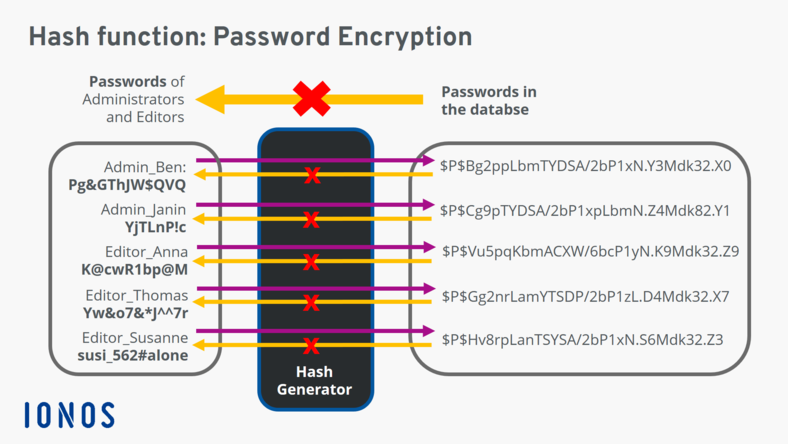
\includegraphics[width=0.6\linewidth]{figs/EstadoArte/Blockchain/hash}
  \caption[Hash]{Ejemplo genérico del funcionamiendo de un algorítmo hash}
  \label{fig:hash}
\end{figure}

\clearpage

Existen múltiples algorítmos hash, y van evolucionando con el tiempo siendo cada vez más seguros y con menos colisiones. Una colisión, se da cuando dos entradas diferentes producen el mismo resultado (rompiendo con una de las reglas principales de los algorítmos hash). \\

Para continuar con la explicación, utilizaremos como ejemplo la red de \textbf{Bitcoin}\cite{whatIsBitcoin} y su algorítmo de consenso \textbf{Proof of Work}\cite{whatIsProofOfWork}. La base es la misma para la inmensa mayoría de redes, sin embargo según el algorítmo de consenso el método difiere ligeramente. Los algorítmos se verán mas adelante. 

\begin{figure}[h!]
  \centering
  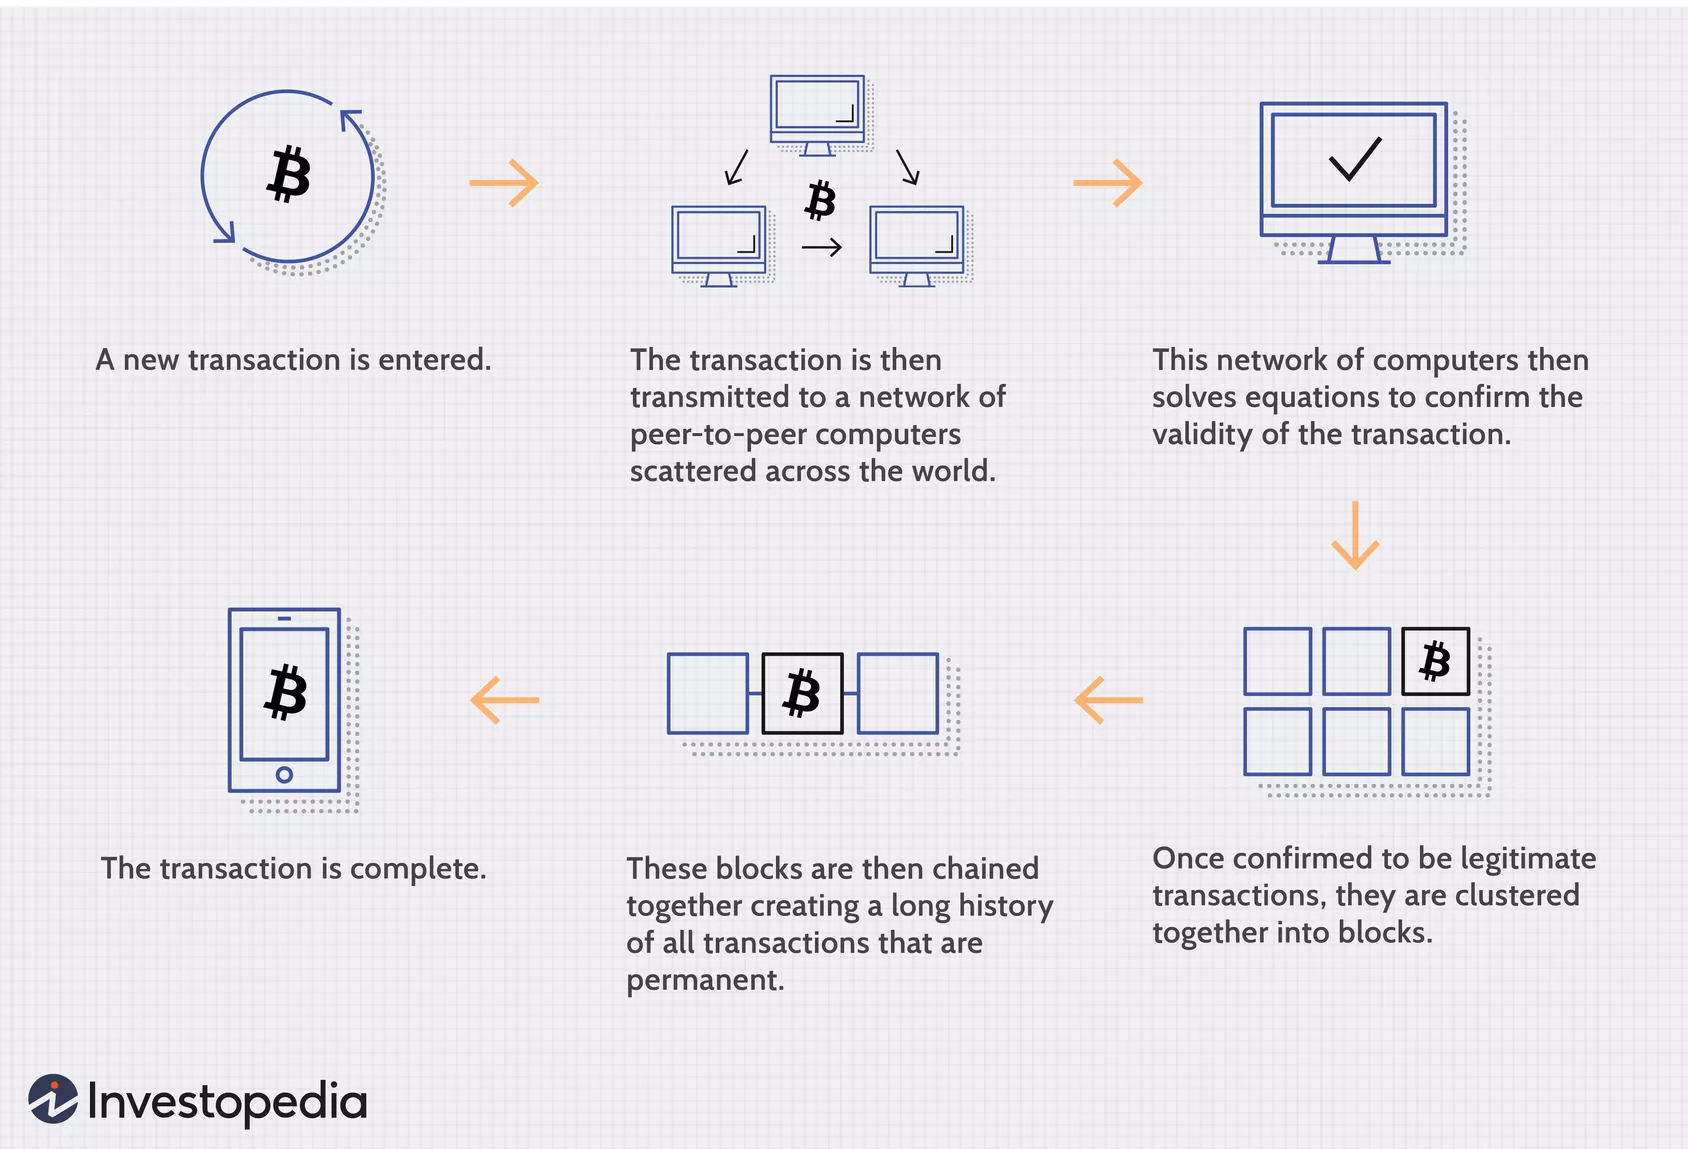
\includegraphics[width=0.8\linewidth]{figs/EstadoArte/Blockchain/bitcoinMining}
  \caption[Bitcoin Mining]{Transaction Process}
  \label{fig:bitcoin}
\end{figure}

Cada bloque de la blockchain, una vez tiene la cantidad de información necesaria para formar un bloque, pasa por una función \textbf{hash256}. Esta información es conocida como ``transacciones'', no son más que datos, ya sean monetarios, envio de datos (nombres, lugares, compras, firmas...) o cualquier tipo de información digital. Todos los nodos de la red comparten estas transacciones, estan todos sincronizados. Él hash por el que pasa la información tiene una especialidad, pues para evitar colisiones entre múltiples nodos de la blockchain, entendemos como nodo un ordenador de la red blockchain, y así evitar que varios bloques se quieran añadir simultaneamente, el hash resultante ha de tener una cantidad determinada de \verb|0|'s al principio del mismo. Por ejemplo, si la dificultad del hash es de \verb|32bits| la función hash256 resultante se puede ver así: \verb|000000003d3a75526946a3bcf00daec9fc9c9c4d51ddc7cc5df888f74dd434d1|. Para llegar a este hash, los nodos de la blockchain tienen que utilizar el hash del bloque anterior junto con la información de las transacciones, y junto con un número conocido como \textbf{nonce}\cite{whatIsNonce}. Un \textbf{nonce} es un número que solo puede ser usado una vez. Los nodos solo pueden modificar este número, no pueden tocar ni el hash del bloque anterior ni las transacciones. Los nodos proceden entonces a modificar de manera aleatoria este nonce hasta dar con el hash con los \verb|0|'s que se piden. Este procedimiento es completamente aleatorio, por lo que a más poder de computo, mas rápido puedes probar números y mas posibilidades tienes de dar con el hash que se pide. A este proceso se le llama ``minado''\cite{minarBitcoin}

\begin{figure}[h!]
  \centering
  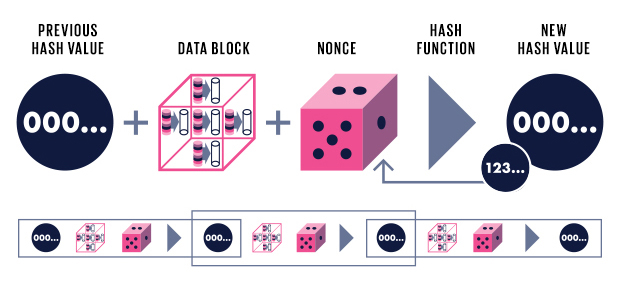
\includegraphics[width=0.8\linewidth]{figs/EstadoArte/Blockchain/hashDificultad}
  \caption[Hash dificultad]{Dificultad del hash}
  \label{fig:hashDiff}
\end{figure}

Una vez un nodo encuentra el nonce correto, lo comparte con el resto de nodos de la red blockchain los cuales validan la información, y se procede a añadir el nuevo bloque a la red blockchain. El nodo que ha encontrado el resultado correcto recibe un incentivo, en el caso de bitcoin, el nodo se asigna a si mismo un número de bitcoins, creando así nuevo bitcoin. 

% -------------------------------------------------- %
\subsection{Tipos de redes blockchain}

Cuando se habla de blockchain, parece dar la impresión de que solo existe un tipo. Sin embargo hay varias redes con sus ventajas y desventajas\cite{tiposBlock1}\cite{tiposBlock2}. Las principales diferencias entre ellas son las \textbf{funcionalidades, protocolos de consenso, administración y reglas para validar las transacciones}.

\subsubsection{Blockchain pública}

Las blockchain públicas no tienen permisos, cualquier usuario es bienvenido a unirse a la red, a enviar transacciones, a utilizar las funcionalidades que tiene la red, y a minar bloques. Las principales características de esta red son:
\begin{itemize}
\item Son \textbf{transparentes}: El código, el funcionamiento interno, los smart contracts si tiene (se verá este término mas adelante) son todos públicos y de código abierto.
\item \textbf{Sin permisos}: Cualquier persona puede unirse a la red sin preguntar. Lo único que tiene que hacer es descargar la red y sincronizarse con los demas nodos.
\item Usuarios \textbf{anónimos} y \textbf{sin administriador}: Nadie se conoce en la red, se trabaja siempre con lo que se conoce como \textbf{address}, que viene a ser un identificador único por miembro de la red para identificarlo. Además, no existe administrador de la red, no hay una persona o grupo que tenga poder sobre la red para hacer cambios de ningún tipo.
\item La información de la red puede ser \textbf{mantenida por todas las personas que lo deseen}. Y al minar nuevos bloques, dependiendo de la red, se ofrece un \textbf{incentivo}.
\end{itemize}

En resumidas cuentas, una blockchain pública es \emph{descentralizada}, \emph{distribuida}, \emph{consensuada}, \emph{abierta} y \emph{segura}. Algunos ejemplos de redes públicas son bitcoin\cite{webBitcoin} y ethereum\cite{webEthereum}

\subsubsection{Blockchain privada}

Las blockchains privadas son permisionadas, esto quiere decir que no cualquier persona puede añadirse como nodo libremente. Requieren de una \textbf{entidad} que ejerza de \textbf{administrador}. La mayoría de usuarios no consideran estas redes como blockchain a causa de esto. El administrador de la red tiene que dar permiso a los usuarios para poder minar, enviar transacciones y participar en general en la red. \\

Admeás, es abitual que los datos esten almacenados en servidores centrales y no abiertos al público. Pudiendo acceder a los bloques de la red solo mediante invitación. \\

Algunos ejemplos de blockchains privadas son R3\cite{webR3}, Ripple\cite{webRipple} y Quorum\cite{webQuorum}

\subsubsection{Blockchain híbrida o federada}

Estas redes son utilizadas por grandes empresas y gobiernos, no estan abiertas al público, teniendo la gestión varias entidades. Además no tienen una criptomoneda asociada y no recompensan por el minado de bloques. Sin embargo el software que utilizan es de código abierto, como puede ser \textbf{Hyperldger, Corda}\cite{webHyper, webCorda}. \\

Como ejemplo tenemos la \emph{Enterprise Ethereum Alliance}, en la que participan el Banco Santander y BBVA. Esta red utiliza la blockchain de Ethereum (pública), sin embargo tienen su propia plataforma privada.

\subsubsection{Blockchain as a Service}

Estas redes blockchain son controladas por un proveedor de servicios como puede ser \emph{Amazon}. Estos proveedores permiten utilizar redes blockchain en la nube, permitiendo a los desarrolladores aprovechar el potencial de las redes blockchain sin la necesidad de invertir en el computo que ello requiere.

% -------------------------------------------------- %
\subsection{Tipos de algoritmo de consenso}

\begin{figure}[h!]
  \centering
  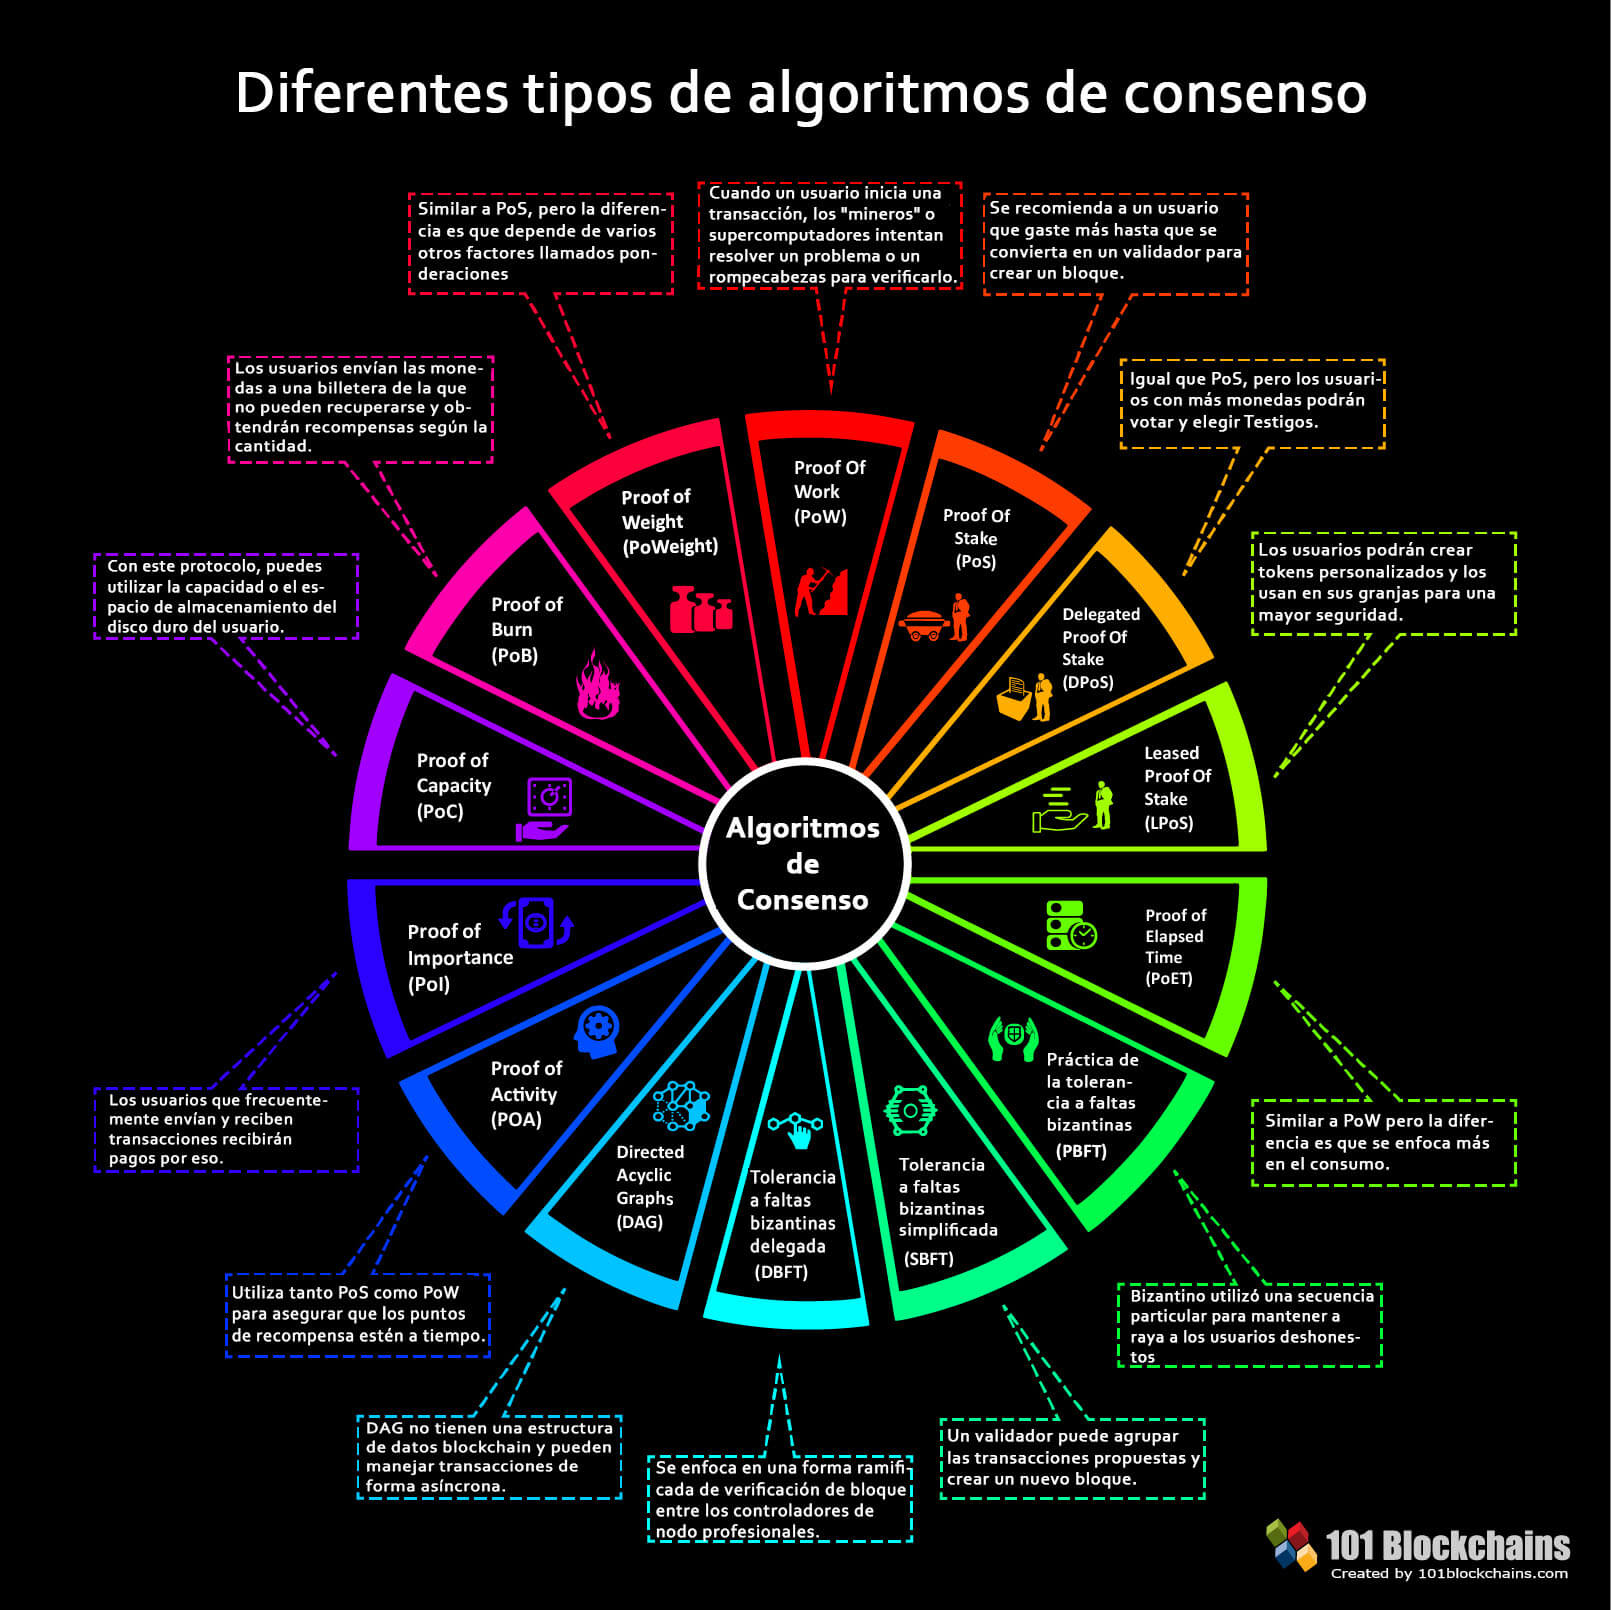
\includegraphics[width=0.8\linewidth]{figs/EstadoArte/Blockchain/algoritmosConsenso.jpeg}
  \caption[Algoritmos de Consenso]{Diferentes tipos de algoritmos}
  \label{fig:consenso}
\end{figure}

Existen múltiples algoritmos de consenso, y estos evolucionan con el paso del tiempo. Los algoritmos de consenso son procesos o protocolos de toma de decisiones, dependiendo del algoritmo hay uno o varios nodos de la red con el poder de tomar la decision sobre que bloque es el siguiente en añadirse a la red y si ha sido o no alterado. Los objetivos que busca blockchain con los algoritmos de consenso son:

\begin{itemize}
\item Llegar a un acuerdo
\item Cooperación
\item Colaboración
\item Igualdad de derechos
\item Participación
\item Actividad
\end{itemize}

Puesto que hay una gran cantidad de algoritmos trataremos de explicar algunos a continuación\cite{algoConsenso}. Todos los algoritmos buscan el mismo objetivo, solucionar el problema de las \textbf{faltas bizantinas}(BFT)\cite{BFT}. La tolerancia a faltas bizantinas es la resistencia de un sistema informático tolerante a fallas de componentes electrónicos. Si lo llevamos al mundo blockchain, cuando hablamos de fallas nos referimos a nodos de la blockchain defectuosos accidentalmente o provocado. Si una empresa tiene control de 200 nodos, puede tratar de crear transacciones falsas y minar ese bloque con los 200 nodos, el resto de nodos de la red tienen que ser capaces a través del algoritmo de consenso que se utilice de descartar la información de estos 200 nodos.

\subsubsection{Proof of Work (PoW)}

El algoritmo de prueba de trabajo es el primer algoritmo introducido en la red blockchain. Muchas blockchains utilizan este algoritmo para llevar a cabo el consenso y así confirmar todas las transacciones. \\ 

\emph{¿Como funciona?} Cada nodo tiene descargada la red blockchain entera, cuando el nuevo bloque tiene las transacciones necesarias para ser minado, todos los nodos se ponene a buscar el resultado de un \textbf{hash} con la dificultad que tenga el mismo. A más poder de computo, mas posibilidades de encontrar el resultado, validarlo con los otros nodos y añadirlo a la red blockchain, además las redes que usan PoW suelen tener un sistema de premios por lo que cuando un nodo encuentra la solución al problema se le da criptomonedas a cambio. \\

Este sistema tiene dos principales desventajas, la primera es que el poder de cálculo que se necesita es muy grande, y estos últimos años han crecido lo que se conoce como granjas de minado las cuales se llevan el premio la gran mayoría de veces. Esto causa que el sistema empiece a centralizarse, rompiendo con la idea de descentralización que tiene blockchain. El problema es que si alguien logra tener él poder de computo de un 51\% de la red blockchain este puede añadir los bloques que quiera a partir de ese momento pues siempre serán validados por la mayoría de nodos (su 51\% de los nodos). La segunda gran pega va liagada a estas granjas de minado, consumen gran cantidad de energía, en 2020 bitcoin consumió \emph{120 gigawatts} por segundo\cite{bitcoinEnergyUse} lo que a nivel medioambiental tiene un impacto negativo, por lo que PoW no es un algoritmo de consenso que se pueda mantener en el tiempo.

\emph{Ventajas y Desventajas}
\begin{itemize}
\item PROS
  \begin{itemize}
  \item Evita ataques DDoS
  \item Es justo y transparente
  \item Fomenta el interés del público en mantener una red saludable
  \end{itemize}
\item CONS
  \begin{itemize}
  \item La adquisición de equipo para el minado es costosa
  \item La máquina destinada al minado no podrá utilizarse para otra tarea pues se necesita todo el poder de computo en la resolución de los problemas matemáticos.
  \item La red tiende a centralizarse a causa de las granjas de minado, dandole poder al dueño de la granja y rompiendo la descentralización.
  \item La minería desaparecerá cuando no haya mas incentivos, en el caso de Bitcoin, cuando se alcance el límite de Bitcoins (21 Millones) los mineros dejarán de recibir premios y se perderá la motivación del minado.
  \end{itemize}
\end{itemize}

\subsubsection{Proof of Stake (PoS)}

El concepto de participación establece que una persona puede minar o validar transacciones en bloque según el número de monedas que posea. Esto significa que cuanta más criptomoneda tengas, más poder de minado se te asigna. \\ 

Se creó como alternativa a PoW, para solventar algunos problemas que tiene (como el de la centralización a causa de las granjas de minado y el gasto energético derivado del poder de computo). PoS solventa este problema atribuyendo la potencia minera a la proporción de monedas que posee un minero. Por lo tanto, en vez de utilizar energía para responder al puzzle matemático como hace PoW, aquí el minero se limita a resolver un porcentaje de las transacciones. Si se tiene un 3\% de las criptomonedas disponibles, se puede minar un 3\% de los bloques, en esta ocasión no hay que resolver ningun puzzle matemático, simplemente generar un \textbf{hash} con los datos, lo que es una tarea trivial. \\

PoS no es una solución definitiva, pues tiene problemas al igual que PoW. Al igual que antes mencionamos el ataque del 51\% (cuando una empresa o alguien tiene un 51\% de los nodos en su poder). En PoS, si tienes un 51\% de las criptomonedas, tienes un 51\% del poder de decision sobre la red, pudiendo hacer los cambios que quieras en ella. Este ataque es frecuente en redes pequeñas con pocas criptomonedas en juego, puesto que de lo contrario, lograr tener un 51\% de las monedas supone tener muchísimo dinero. Para controlar estas fraudulencias, se penaliza económicamente a los nodos que tratan de saltarse las reglas (modificar bloques y transacciones), además, un ataque a la blockchain afecta al poder de la moneda y por lo tanto su valor en mercado disminuye, por lo que no compensa tratar de burlar las reglas de la blockchain. Los nodos de las redes que usan PoS, reciben una comisión al minar correctamente su parte del bloque. \\

Redes que utilizan este algoritmo son: Ethereum2.0\cite{Ethereum2.0} y NxT\cite{NxT}.

\subsubsection{Proof of Elapsed Time (PoET)}

La prueba de tiempo transcurrido es un algoritmo que evita la alta utilización de recursos y el alto consumo de energía manteniendo el proceso más eficiente. El algorítmo utiliza un tiempo transcurrido generado aleatóriamente para decidir los derechos de minería y los ganadores de los bloques. Al ejecutar un código de confianza dentro de un entorno seguro, el algoritmo PoET también mejora la transparencia al garantizar que los resultados sean verificables por participantes externos. Este algorítmo se utiliza en redes blockchain permisionadas, por lo que se conoce al dueño de cada nodo. \\

Cada nodo participante en la red debe esperar durante un periodo de tiempo elegido al azar, y el primero en completar el tiempo de espera designado gana el nuevo bloque. Cada nodo de la red blockchain genera un tiempo de espera aleatorio y se pone a dormir durante esa duración especificada. El que se despierta primero, es decir, el que tiene el tiempo de espera más corto, se despierta y consigna un nuevo bloque en la cadena de bloques, transmitiendo la información necesaria a toda la red de pares. El mismo proceso se repite para descubrir el siguiente bloque. \\

% -------------------------------------------------- %
\subsection{Smart contracts}

Hasta ahora, hemos hablado de blockchain y criptomonedas, pero las criptomonedas son solo un muy pequeño uso del potencial de blockchain. Los \textbf{Smart Contracts}\cite{etherSmartContract} son un programa que se ejecuta en la red blockchain dando así la capacidad a la red de ser más versatil, al poder ejecutar código (escrito en el smart contract). Básicamente, añade una lógica a la blockchain. \\

Una forma de entender los smart contracts es comparandolos a una máquina de ventas automática. Cuando quieres un snack introduces dinero en la máquina y pones el código del snack, la máquina tiene programada una rutina para verificar que has metido la cantidad adecuada y a cambio devuelve el snack seleccionado. Ese programa interno que tiene la máquina, es el equivalente a un \textbf{smart contract}. \\

Los smart contract son muy poderosos al estar programados en la red blockchain no pueden ser modificados sin que todos los nodos se enteren. Si un nodo trata de modificar el smart contract, se creará una transacción la cual ha de ser validada por todos los nodos, al igual que cuando hablabamos de cambiar transacciones en criptomonedas, los algoritmos de consenso se encargarán de prohibir que nodos no permitidos cambien componentes del smart contract. \\

Los smart contracts permiten que se realicen transacciones y acuerdos de confianza entre partes dispares y anónimas sin necesidad de una autoridad central, un sistema legal o un mecanismo de aplicación externo. \\

\label{sec:smartContract}
\index{SmartContract}

\begin{lstlisting}[language=Java,float=ht,caption={[Smart Contract]Ejemplo de código fuente de un smart contract escrito en Solidity},label=lst:java]
pragma solidity 0.6.11;

contract VendingMachine {

    // Declare state variables of the contract
    address public owner;
    mapping (address => uint) public cupcakeBalances;

    // When 'VendingMachine' contract is deployed:
    // 1. set the deploying address as the owner of the contract
    // 2. set the deployed smart contract's cupcake balance to 100
    constructor() public {
        owner = msg.sender;
        cupcakeBalances[address(this)] = 100;
    }

    // Allow the owner to increase the smart contract's cupcake balance
    function refill(uint amount) public {
        require(msg.sender == owner, "Only the owner can refill.");
        cupcakeBalances[address(this)] += amount;
    }

    // Allow anyone to purchase cupcakes
    function purchase(uint amount) public payable {
        require(msg.value >= amount * 1 ether, "You must pay at least 1 ETH per cupcake");
        require(cupcakeBalances[address(this)] >= amount, "Not enough cupcakes in stock to complete this purchase");
        cupcakeBalances[address(this)] -= amount;
        cupcakeBalances[msg.sender] += amount;
    }
}
\end{lstlisting}

Los smart contracts pueden ser escritos en múltiples lenguajes de programación dependiendo de la red blockchain que se vaya a utilizar. Algunos ejemplos son:
\begin{itemize}
\item EOS Blockchain -> \verb|C++|
\item Ethereum -> \verb|Solidity|
\item NEO Blockchain -> \verb|JavaScript, Java|
\item Hyperldger -> \verb|Golang|
\item Cardano -> \verb|Haskell|
\end{itemize}

La primera red blockchain en explotar el potencial de los smart contracts fue \textbf{ethereum} y puesto que es la red blockchain sobre la cual se apoyará la aplicación Android que voy a desarrollar en este TFG, procederé a analizarla.

% -------------------------------------------------- %
\subsection{Usos en el presente de Blockchain}
En el presente estan en desarrollo múltiples aplicaciones basadas en Blockchain:

\begin{itemize}
\item Criptomonedas: \emph{Bitcoin, Ethereum, Tether, Cardano, XRP, Litecoin, ChainLink, Dogecoin, TRON, VeChain, Monero, BitTorrent, Kusama, Neo, Dai, NEM, Dash, Maker}\dots \cite{listaCripto}.
\item Firma digital y verificación de la identidad: Startups como \emph{Civic} o \emph{Niuron}\cite{civic, niuron} buscan implementar firmas digitales para notarios y bancos y check-in telemáticos en hoteles y pisos turísticos.
\item Trazabilidad alimentaria: Empresas como carrefour implementan trazabilidad de sus alimentos con la ayuda de IBM \cite{carrefour}
\item Turismo y Hoteles: La empresa \emph{TUI Group} cuenta con más de 300 hoteles y esta moviendo sus activos inmobiliarios y procesos internos a una blockchain \cite{tuig}.
\item Votaciones y elecciones: El \emph{banco santander} utilizó en 2018 con éxito una red blockchain para votar a su Junta General de Accionistas\cite{santanderVotacion}
\end{itemize}

Y mucho más \cite{appCripto}.

% -------------------------------------------------- %
\section{Ethereum}

\begin{figure}[h!]
  \centering
  
\includegraphics[width=0.6\linewidth]{figs/EstadoArte/Ethereum/ethereumLOGO}
  \caption[Ethereum]{Logo de ethereum}
  \label{fig:ethereum}
\end{figure}

Ethereum es una red blockchain que permite enviar criptomonedas a cualquier persona por una pequeña comisión. Admeás permite ser programada con ayuda de los smart contracts, permitiendo así desarrollar aplicaciones sobre la red blockchain. \\

% -------------------------------------------------- %
\subsection{Ether (ETH)}
La moneda que utiliza la red de Ethereum es el \textbf{ether}, se utiliza para compensar a los mineros que aseguran las transacciones. Recordemos, \emph{Ethereum1.0 utiliza PoW} pero \emph{Ethereum2.0 utiliza PoS}\cite{Ethereum2.0}. Los ethers se utilizan como almacén de valor, prestamos de garantía, medio de intercambio, unidad de cuenta en mercados digitales \dots \\

Cada transacción en ethereum lleva asociado un coste conocido como \textbf{gas}. El gas es la unidad que se utiliza para ver el coste de computo que tiene la transacción, para poder remunerar adecuadamente al minero. La unidad de gas se mide en \textbf{Gwei}\cite{Gwei} si por ejemplo queremos enviar una cantidad \verb|X| de ether a otra persona esta transacción tiene un coste de \verb|21.000|Gwei lo que es equivalente a \verb|0,000021 ETH| (1ETH = $10^9$Gwei)

% -------------------------------------------------- %
\subsection{Carteras}

Las carteras de ethereum son aplicaciones que permiten a los ususarios interactuar con sus cuentas de ethereum. Se las puede ver como una aplicación bancaria. Tu cartera te permite leer tu saldo, enviar transacciones y conectarte a aplicaciones. Se necesita una cartera para enviar fondos y gestionar tu ETH. Pero es únicamente una herramienta para gestionar tu cuenta, puedes cambiar de cartera sin problema pues no es quien custodia tus fondos, eres tú quien los custodia en todo momento. \\

La cartera tiene asociado un \textbf{address}, un address es el identificador que tiene tu cuenta en la red de ethereum, es único para tí. Si alguien quiere enviarte dinero lo hará desde su address a tú address, si quieres hacer una llamada a un Smart Contract, al smart contract le llegará como información tú address. \\

Tres términos importantes:
\begin{itemize}
\item \textbf{Cuenta} de ethereum.
\item \textbf{Address} de la cuenta.
\item \textbf{Cartera} para gestionar la cuenta.
\end{itemize}

% -------------------------------------------------- %
\subsection{Ethereum Smart Contract}

Los smart contracts de ethereum están escritos en \textbf{Solidity}\cite{SolidityDocs} o \textbf{Vyper}\cite{VyperDocs}. Cualquier persona es libre de programar un smart contract y desplegarlo en la red de ethereum, los smart contracts son una transacción más y tienen su propio address. Permitiendo que cualquier persona hacer llamadas al smart contract. Desplegar un smart contract cuesta \emph{gas} al igual que cualquier transacción, sin embargo es bastante más caro. 

\begin{figure}[hbt]
	\centering
	\begin{subfigure}[b]{0.4\linewidth}
		\centering
		
\includegraphics[width=0.8\linewidth]{figs/EstadoArte/Ethereum/solidityLOGO}
		\caption{Logo de Solidity}\label{fig:solProgram}
	\end{subfigure} 
	\begin{subfigure}[b]{0.4\linewidth}
		\centering
		
\includegraphics[width=0.8\linewidth]{figs/EstadoArte/Ethereum/vyperLOGO}
		\caption{Logo de Vyper}\label{fig:vyperProgram}
	\end{subfigure} 
	\caption[Lenguajes de Smart Contract]{Lenguajes de smart contract para ethereum.}
	\label{fig:programas}
\end{figure}

\clearpage

\label{sec:solidity}
\index{Solidity}

\begin{lstlisting}[language=Java,float=ht,caption={[Solidity Contract]Ejemplo de código fuente de un smart contract escrito en Solidity},label=lst:java]
// SPDX-License-Identifier: GPL-3.0
pragma solidity >= 0.7.0;

contract Coin {
    // The keyword "public" makes variables
    // accessible from other contracts
    address public minter;
    mapping (address => uint) public balances;

    // Events allow clients to react to specific
    // contract changes you declare
    event Sent(address from, address to, uint amount);

    // Constructor code is only run when the contract
    // is created
    constructor() {
        minter = msg.sender;
    }

    // Sends an amount of newly created coins to an address
    // Can only be called by the contract creator
    function mint(address receiver, uint amount) public {
        require(msg.sender == minter);
        require(amount < 1e60);
        balances[receiver] += amount;
    }

    // Sends an amount of existing coins
    // from any caller to an address
    function send(address receiver, uint amount) public {
        require(amount <= balances[msg.sender], "Insufficient balance.");
        balances[msg.sender] -= amount;
        balances[receiver] += amount;
        emit Sent(msg.sender, receiver, amount);
    }
}
\end{lstlisting}

% -------------------------------------------------- %
\subsection{Funcionamiento básico de Ethereum}

Para entender el funcionamiento básico de Ethereum, vamos a exponerlo por niveles como lo hacen en la documentación oficial\cite{etherStack}. 

% -------------------------------------------------- %
\subsection{Nivel 1: Máquina Virtual de Ethereum} 

La \textbf{EVM} es el entorno de ejecución de los smart contract. Esta, gestiona todo el procesamiento de transacciones en la red, creando un nivel de abstracción entre el código que se ejecuta y la máquina que lo hace. La EVM es \emph{Turing-Completa} con 140 instrucciones únicas que la permiten ejecutar casi cualquier cosa. 

\begin{figure}[h!]
  \centering
  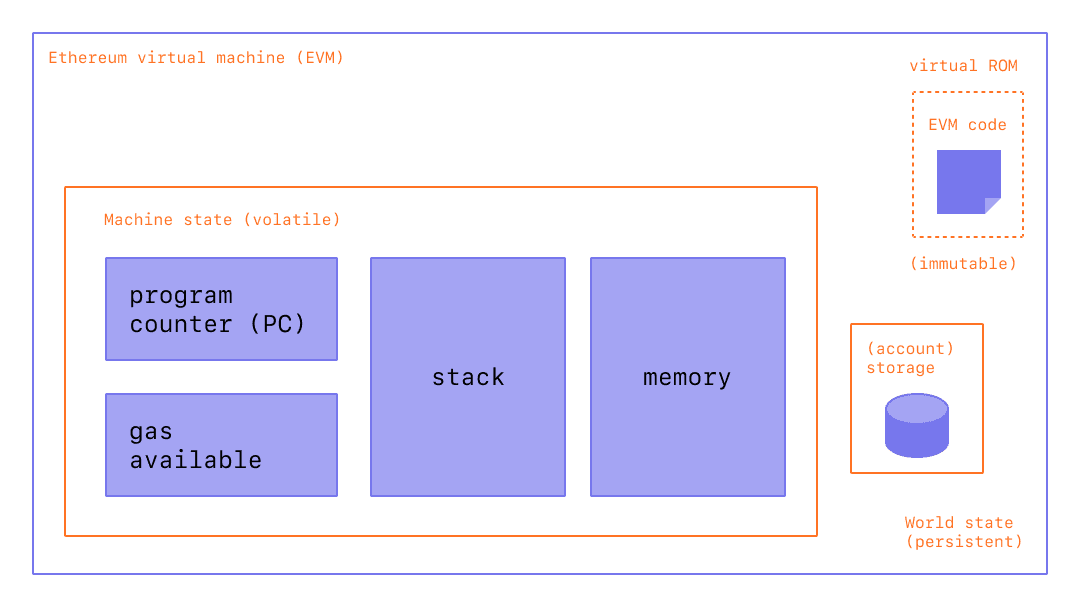
\includegraphics[width=0.6\linewidth]{figs/EstadoArte/Ethereum/evm}
  \caption[Diagrama EVM]{Diagrama de la máquina virtual de ethereum}
  \label{fig:evm}
\end{figure}

% -------------------------------------------------- %
\subsection{Nivel 2: Smart Contract} 

Programas que se ejecutan en la red de ethereum. 

% -------------------------------------------------- %
\subsection{Nivel 3: Nodos de Ethereum}

Para que una app pueda interactuar con la red, necesita conectarse a un nodo de ethereum. Los nodos son ordenadores que ejecutan el \emph{software} cliente de ethereum, manteniendo el registro de bloques y validando las transacciones. Almacenan colectivamente el estado de la blockchain y llegan a un consenso sobre las transacciones para hacer crecer el número de bloques. Al conectar la app con un nodo, la app puede leer datos de la red, enviar nuevas transacciones\dots

\begin{figure}[h!]
  \centering
  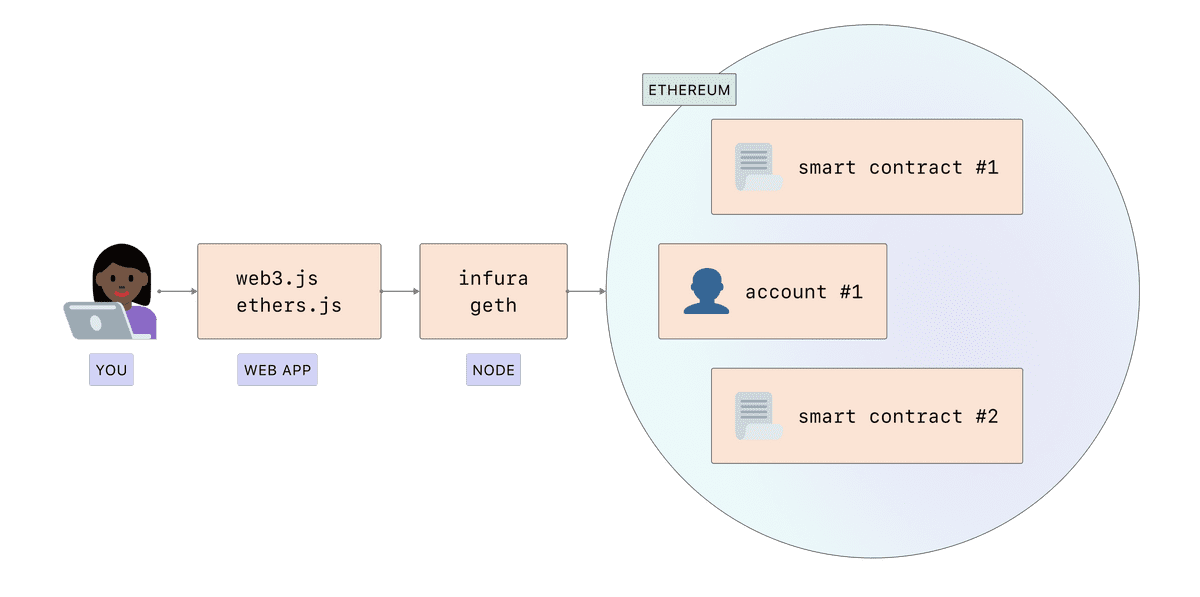
\includegraphics[width=0.6\linewidth]{figs/EstadoArte/Ethereum/ethereumNodo}
  \caption[Nodos vista genérica]{Nodo y vista genérica de aplicaciones.}
  \label{fig:etherNodo}
\end{figure}

% -------------------------------------------------- %
\subsection{Nivel 4: API para el cliente de ethereum}

Las APIs permiten a los desarrolladores absatraer parte de la dificultad de interactuar directamente con los nodos de ethereum. Además proporcionan herramientas como para convertir datos de ETh a Gwei\dots Existen APIs en \verb|JavaScript, Java, Python| por ejemplo, una de las más conocidas es \textbf{Web3}\cite{web3}

% -------------------------------------------------- %
\subsection{Nivel 5: Aplicaciones para usuario}

En el nivel superior estan las apps orientadas al usuario. Principalmente son aplicaciones web y móvil. Las aplicaciones se contruyen de la manera tradicional, y utilizan las APIs necesarias para comunicarse con la red y/o smart contracts.

% -------------------------------------------------- %
% -------------------------------------------------- %
\section{Aplicaciones móvil que usan Blockchain}

Ahora que entendemos que es Blockchain, visto múltiples ejemplos de redes, visto múltiples aplicaciones de la red Blockchain, y hemos indagado más sobre Ethereum y lo Smart Contract, vamos a pasar a ver los proyectos actuales que utilizan aplicaciones móvil y blockchain. Puesto que el objetivo de este \textbf{TFG} es el desarrollo de una aplicación Android que comunique con una blockchain. 

% -------------------------------------------------- %
\subsection{GUTS Tickets}

Esta aplicación móvil usa blockchain para emitir entradas honestas que ponen fin a los vergonzosos precios del mercado de la ``reventa'' y al fraude en las entradas. \emph{GUTS} es el primer sistema de ventas de entradas que hace uso del \textbf{Protocolo de Entrada Garantizada} {\small (\emph{Guaranteed Entrance Protocol (GET)})}\cite{GET}. Este protocolo permite crear entradas inteligentes y seguras permitiendo el seguimiento de las mismas así como el control de su precio original y secundario (reventa). 

\begin{figure}[hbt]
	\centering
	\begin{subfigure}[b]{0.4\linewidth}
		\centering
		
\includegraphics[width=0.8\linewidth]{figs/EstadoArte/Apps/getTOKEN.png}
		\caption{Logo del token de GET}\label{fig:getTOKEN}
	\end{subfigure} 
	\begin{subfigure}[b]{0.4\linewidth}
		\centering
		
\includegraphics[width=0.8\linewidth]{figs/EstadoArte/Apps/gutsLOGO.png}
		\caption{Logo de la aplicación Guts}\label{fig:gutsLOGO}
	\end{subfigure} 
	\caption[Logos de Guts y GET]{Logos}
	\label{fig:Logos}
\end{figure}

\subsubsection{Protocolo GET}

El protocolo GET ofrece una solución de emisión de billetes inteligentes basadas en blockchain que puede ser utilizada por todos los que necesitan emitir billetes de forma transparente, segura y honesta. Evitando fraudes, y vergonzosas subidas del precio de las entradas en el mercado de la reventa. La funcionalidad de registro de entradas de GET funciona con un SmartContract escrito en solidity, su codigo fuente es de código abierto \cite{srcGET}. La blockchain que utiliza para apoyarse es la de \emph{Ethereum}, y disponen de \textbf{Token} propio para realizar las transacciones\cite{tokGET}. GET guarda un historial para cada tickets utilizando \textbf{IPFS}\cite{IPFS} que luego guarda en la red blockchain con el smart contract, \emph{sobre IPFS, pretende superar a HTTP para contruir una web mejor para todos}.

% -------------------------------------------------- %
\subsection{LifeID}

Esta aplicación esta construyendo una plataforma de identidad digital segura y basada en blockchain. Con una sencilla aplicación móvil te ofrece el control sobre la gestión de tú identidad digital. Permite iniciar sesión en cualquier sitio, entrar en cualquier edificio en el que se requiera de autenticación o participar en transacciones basadas en la identidad (como puede ser en un sistema de votación) todo con la tranquilidad, fiabilidad y control que da la blockchain. \\ 

Para ello utiliza la red blockchain de \textbf{ArcBlock}\cite{webArc,alianzaArc}. ArcBlock es una plataforma para desarrollar aplicaciones en blockchains conocidas como \textbf{DApps}\cite{dapps}. 



\chapter{Desarrollo}
\label{cap:Desarrollo}

\setlength{\parindent}{0pt}

En este capítulo se hablará del desarrollo de la aplicación (diseño, funcionalidades, librerías, gestión del wallet, documentación\dots) que se ha estado realizando a lo largo del TFG, así como el registro de claves para poder interactuar con la red blockchain que se ha levantado. También, se explicará en que consiste el SDK desarrollado, cuales son sus funcionalidades y como poder utilizarlo en otras aplicaciones Android. \\

El desarrollo de la aplicación móvil, se ha enfocado únicamente a dispositivos Android. Lógicamente, en un futuro, se tendrá que adaptar una aplicación para otros sistemas operativos como iOS. O por el contrario reescribir él código con lenguajes ``cross platform'' para permitir el correcto funcionamiento nativo tanto en Android como en iOS, una buena opción es utilizar \textbf{flutter}\cite{flutter}.

% ##################################################
% ##################################################
\section{Arquitectura de la Aplicación}

Recordemos un poco el esqueleto del proyecto ``Estublock''. Se ha decidido crear varios componentes modulares soportados por APIs, así cambios en el código de un componente no afectan al resto. El proyecto dispone de tres APIs diferentes. Tenemos primero la API que comunica con el servidor que tiene ejecutando la base de datos, luego la API que trata algunos datos con la red blockchain que se ha levantado. Y por último, una API intermedia que es con la que se comunica el dispositivo móvil para centralizar las llamadas, quitarle trabajo de computo al móvil y a la aplicación. Sin embargo, recordemos que el dispositivo móvil también hará llamadas directamente a la red blockchain a través del \hyperref[sec:SDK]{SDK}. La arquitectura queda como se muestra en la figura \ref{fig:estublockArch}. \\

El dispositivo móvil se comunica entonces con la api de microservicios con la ayuda de dos librerías que veremos más en profundidad en el apartado de \hyperref[sec:Codigo]{Codigo}, esta API a su vez se comunica con la API de la base de datos o de la red blockchain según la operación que se haya especificado y estas se comunican con el servidor postgresql para la base de datos y la red de quorum para la blockchain. \\

\begin{figure}[h!]
  \centering
  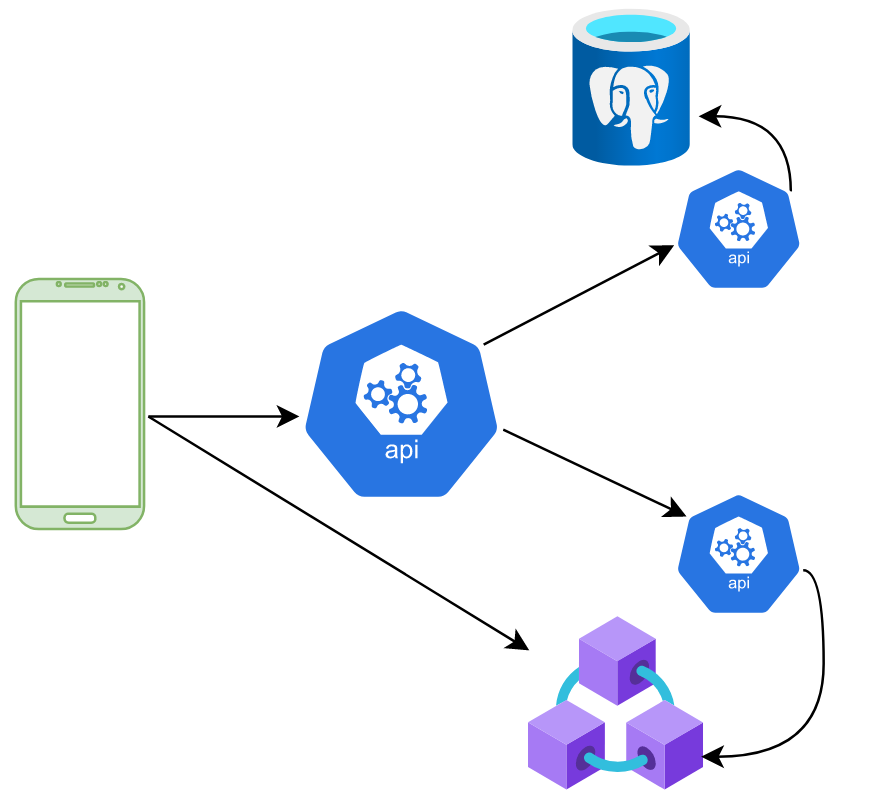
\includegraphics[width=0.4\linewidth]{figs/Desarrollo/Arquitectura}
  \caption[Arquitectura]{Arquitectura Completa del proyecto}
  \label{fig:estublockArch}
\end{figure}

% --------------------------------------------------
\section{Interaz de Usuario}

La interfaz de usuario es donde los usuarios interaccionan con la aplicación. Son las ventanas, botones, pantallas con las que el usuario interacciona. Deben tener un diseño intuitivo, fácil, que brinde una experiencia positiva. A más fácil de entender, mejor. Existen tres grandes tipos de interfaces de usuario, la interfaz de lenguaje natural, es la ideal y el sueño de todo usuario, pues permite comunicar humano y máquina con lenguaje natural. Un ejemplo de dispositivo que utiliza esta interfaz es \emph{Alexa}, que cuenta con un software basado en modelos acústicos y del lenguaje. El segundo tipo de interfaz es la interfaz de preguntas y respuestas. En esta interfaz se muestra una pregunta al usuario y según su respuesta se actúa de una u otra manera. Un ejemplo de estas interfaces son los software de instalación, como puede ser el instalador de un sistema operativo. Y por último, la interfaz que más nos interesa para este proyecto, la \textbf{interfaz gráfica de usuario}, en inglés ``Graphical User Interface'' o \textbf{GUI}. Esta utiliza gráficos, imágenes, videos, iconos, menús\dots para permitir al usuario interaccionar con la aplicación. 

\subsection{Interfaces Gráficas en Android} \label{sec:GUI}

En Android la interfaz de usuario se construye mediante una jerarquía de objetos, generalmente de tipo \textbf{View y ViewGroup}. Los \emph{View} son componentes con los que el usuario puede interactuar, el usuario puede ver el componente en la pantalla. Sin embargo los \emph{ViewGroup} son un contenedor invisible que define la estructura de objetos \emph{View} y otros \emph{ViewGroup}, un árbol jerárquico puede verse en la figura \ref{fig:interfaz_android}.

\begin{figure}[h!]
  \centering
  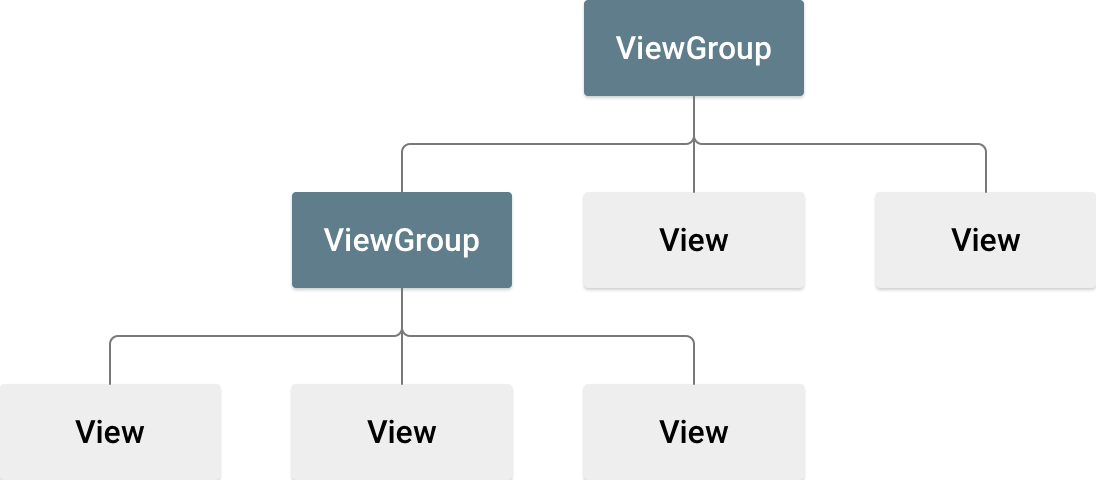
\includegraphics[width=0.75\linewidth]{figs/Desarrollo/Jerarquia}
  \caption[Android Layout]{Jerarquia de una interfaz de Android}
  \label{fig:interfaz_android}
\end{figure}

Los objetos \emph{View} se denominan ``widgets'' y pueden ser Botones, Textos, ``Switch'', ``ScrollView''\dots Los objetos \emph{ViewGroup} se denominan ``diseño'' y pueden ser ``LinearLayout'', ``ConstraintLayout''\dots Los diseños se pueden declarar de dos maneras, podemos declararlos con antelación, esto es programar en código XML como queremos que se vea una pantalla. Y también se pueden instanciar desde el código en tiempo de ejecución y modificar datos de la pantalla, o crear nuevos datos que no hay, (los datos pueden ser botones, cajas, menus, desplegables\dots). \\

Para la aplicación, se han usado ambas formas, pues por un lado hay pantallas estáticas, como pueden ser la pantalla de login o registro. En las que se sabe que botones tiene que haber, que textos tiene que mostrar y que diseño tiene con antelación. Pero también hay pantallas en las que se crean botones o texto de forma dinámica, por ejemplo, en pantallas que muestran próximos eventos, se muestra de forma dinámica (según el número de eventos que devuelva la API) más o menos botones. \\

Uno de los puntos fuertes de programar con antelación la interfaz con XML, es que se puede separar la presentación de la app del código que controla los componentes, además, facilita la creación de distintos diseños para diferentes tamaños de pantalla, orientación, colores\dots Es la mejor opción a la hora de crear una interfaz de usuario aunque en ocasiones se requiera de crear o modificar de forma dinámica en tiempo de ejecución algunos elementos. También es habitual crear con XML un diseño estático, y luego modificarlo en tiempo de ejecución según sea necesario accediendo a sus componentes.  

% --------------------------------------------------
\subsection{Diseño de la Interfaz de Estublock}

A la hora de diseñar la aplicación Estublock, se ha buscado un diseño ligero, intuitivo y rápido. Como que tener en cuenta a muchos usuarios, hay que pensar en los posibles problemas de visión, daltonismo, dislexia, evitar que se pueda mal interpretar un botón\dots todo esto para evitar en la medida de lo posible que el usuario se lleve una mala experiencia con la aplicación. Para todo ello, se ha utilizado una herramienta de diseño para prototipos de pantallas y testeo de pantallas llamada \emph{Marvelapp}\cite{marvelapp}. Marvelapp permite diseñar con bastante detalle aplicaciones móvil y web, y además permite enlazar pantallas para probar la efectividad de las pantallas y el entendimiento de las mismas. Marvelapp tiene un gran potencial al permitir diseñar rápidamente pantallas y poder probar su efectividad rápidamente. \\

\subsubsection{Pantalla de Registro}

En la pantalla de registro, se pide al usuario que introduzca sus datos personales. Se comprueba que los datos sean correctos, por ejemplo, al introducir el correo electrónico, un \textit{regex} se encarga de verificar que el correo sea universitario. Los regex evalúan expresiones regulares y se puede buscar con él un patrón como puede ser \textit{@alumnos.upm.es} para verificar que el usuario es por ejemplo un alumno. El regex que se ha utilizado para comprobar el correo se muestra en la figura \ref{fig:regex}. \\

\begin{figure}[h!]
  \centering
  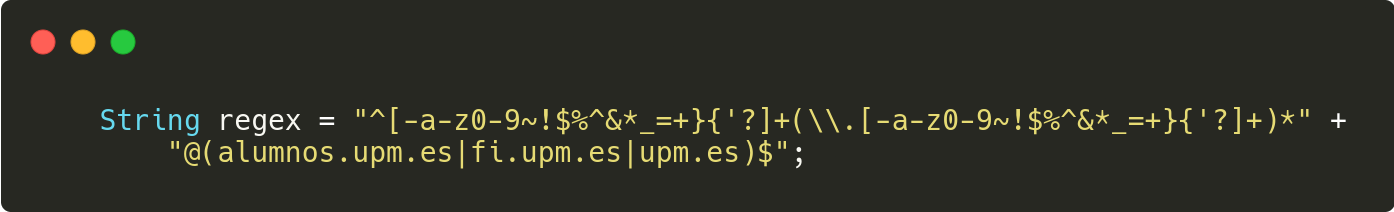
\includegraphics[width=0.9\linewidth]{figs/Desarrollo/Codigo/regex}
  \caption[Código regex de verificación de correo]{Código regex de verificación de correo}
  \label{fig:regex}
\end{figure}

También, se hace verificación de que la contraseña ha sido escrita correctamente dos veces. Esta es una \textbf{nueva} decisión de diseño, puesto que en un inicio como veremos mas adelante, no se contemplaba en la pantalla de registro pedir la contraseña dos veces. Además, otros cambios que ha sufrido la pantalla de registro es en el número de datos que se le piden al usuario. Se ha eliminado la matrícula, esto es temporal, pues es probable que se añada en el futuro. La principal razón que nos llevó a tomar esta decisión, es que los profesores o ponentes de charlas que fuesen a utilizar esta aplicación, no disponen de matrícula. Solo los estudiantes tienen matrícula. Por otro lado, el nombre y apellidos se piden de forma conjunta, esto también es temporal pues hay que estudiar si van a ser o no datos fundamentales para poder acreditar al alumno la asistencia a un evento, o no es tan importante conocer el primer y segundo apellido del usuario, pues al final lo más importante es el correo electrónico. El diseño con \emph{marvelapp} y el resultado final, pueden encontrarse en la figura \ref{fig:pantalla_registro}

\begin{figure}[hbt]
	\centering
	\begin{subfigure}[b]{0.4\linewidth}
		\centering
        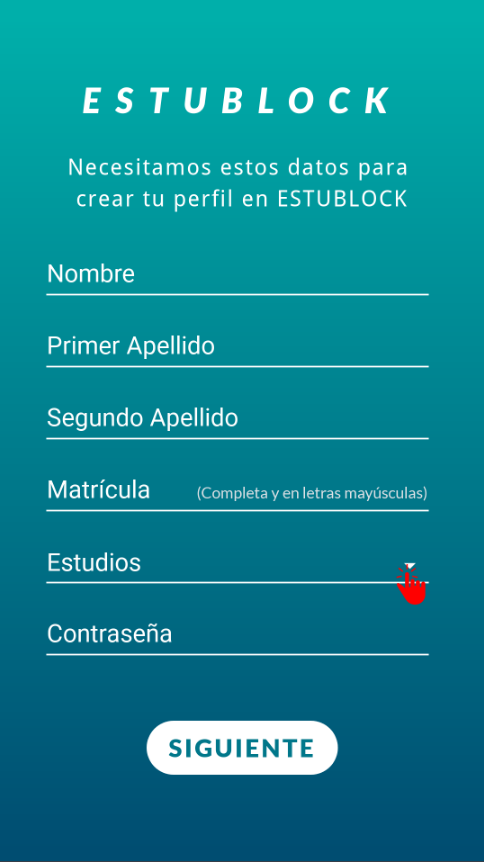
\includegraphics[width=0.7\linewidth]{figs/Desarrollo/Interfaz/marvel_registro}
        \caption[Marvel Registro]{Pantalla de registro de marvelapp}
	\end{subfigure} 
	\begin{subfigure}[b]{0.4\linewidth}
		\centering
        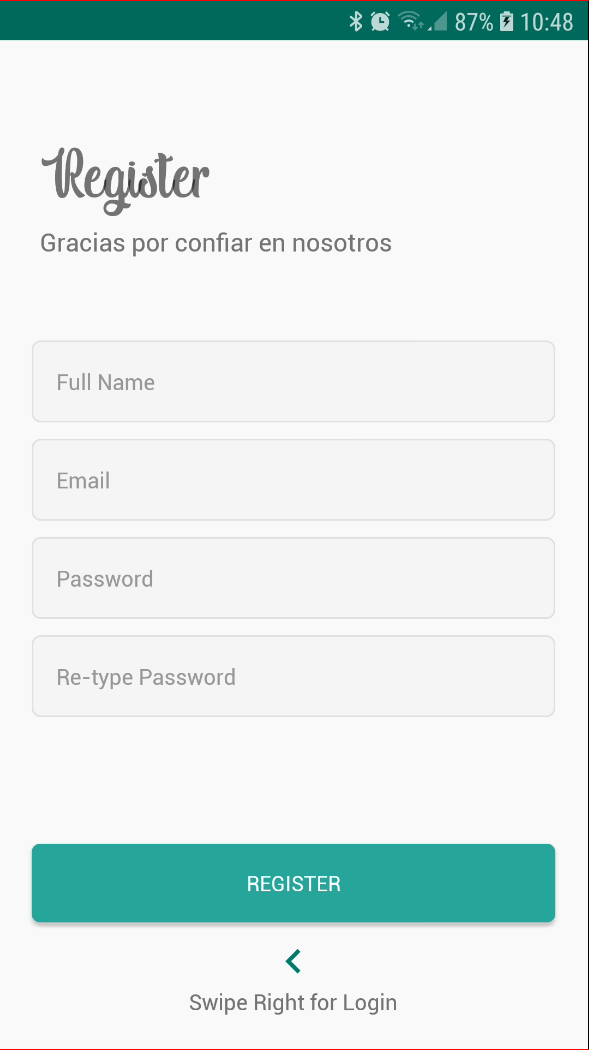
\includegraphics[width=0.7\linewidth]{figs/Desarrollo/Interfaz/estublock_registro}
        \caption[Estublock Registro]{Pantalla de registro de Estublock}
	\end{subfigure} 
	\caption[Pantalla de Registro]{Pantalla de Registro}
	\label{fig:pantalla_registro}
\end{figure}

\subsubsection{Pantalla de Login}

En la pantalla de login, los usuarios pueden iniciar sesión, desbloqueando además su wallet. Este término y sus detalles se verán en el apartado \hyperref[sec:wallet]{Wallet}. Al hacer login, los usuarios solo necesitan introducir el correo electrónico con el que se dieron de alta y la contraseña. Como se puede observar en la figura\ref{fig:pantalla_login} en \emph{Marvelapp} se añadió la opción de recuperar la contraseña del usuario. Sin embargo, no existe en la versión final. \\

Para poder recuperar la contraseña de un usuario, lo normal en un servicio es enviarle un correo electrónico al usuario (al correo que el usuario utilizaó para darse de alta) y desde ese correo el usuario accede a un portal en el que puede modificar su contraseña. Y la contraseña modificada se pasa por una función \textit{hash}\cite{whatIsHash} y se almacena en una base de datos. En el caso de Estublock, a pesar de poder implementar dicho servicio sin problema, y modificar en la base de datos el hash de la contraseña. No serviría de nada, pues la contraseña que se utiliza para desbloquear y utilizar el wallet no puede ser modificada, si el usuario pierde o se le olvida la contraseña, el wallet queda invalidado. Existen dos principales métodos para recuperar el acceso al wallet, estos se verán en el apartado \hyperref[sec:wallet]{Wallet}. Por lo tanto, ante este problema, la pantalla de login final no tiene opción de recuperar las credenciales por ahora. Pues se puede implementar uno de los métodos de recuperación de wallets disponibles. Tanto la pantalla original como la final se pueden ver en la figura \ref{fig:pantalla_login}. \\

\begin{figure}[hbt]
	\centering
	\begin{subfigure}[b]{0.4\linewidth}
		\centering
        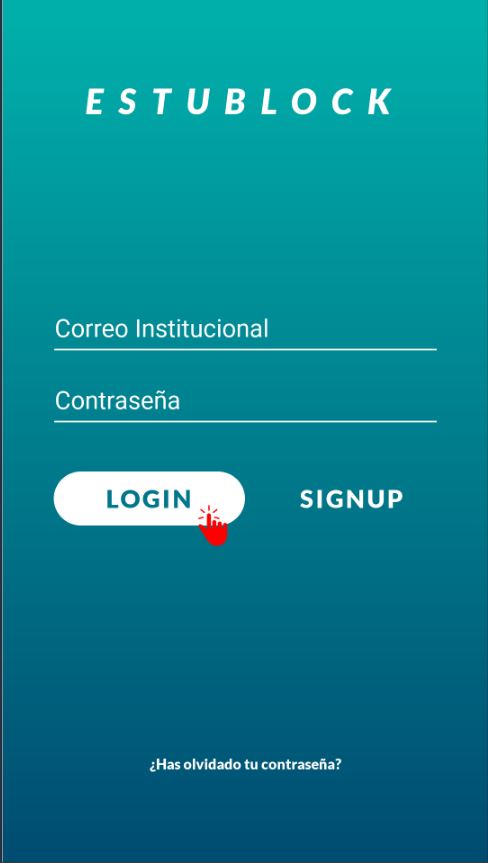
\includegraphics[width=0.7\linewidth]{figs/Desarrollo/Interfaz/marvel_login}
        \caption[Marvel Login]{Pantalla de login de marvelapp}
	\end{subfigure} 
	\begin{subfigure}[b]{0.4\linewidth}
		\centering
        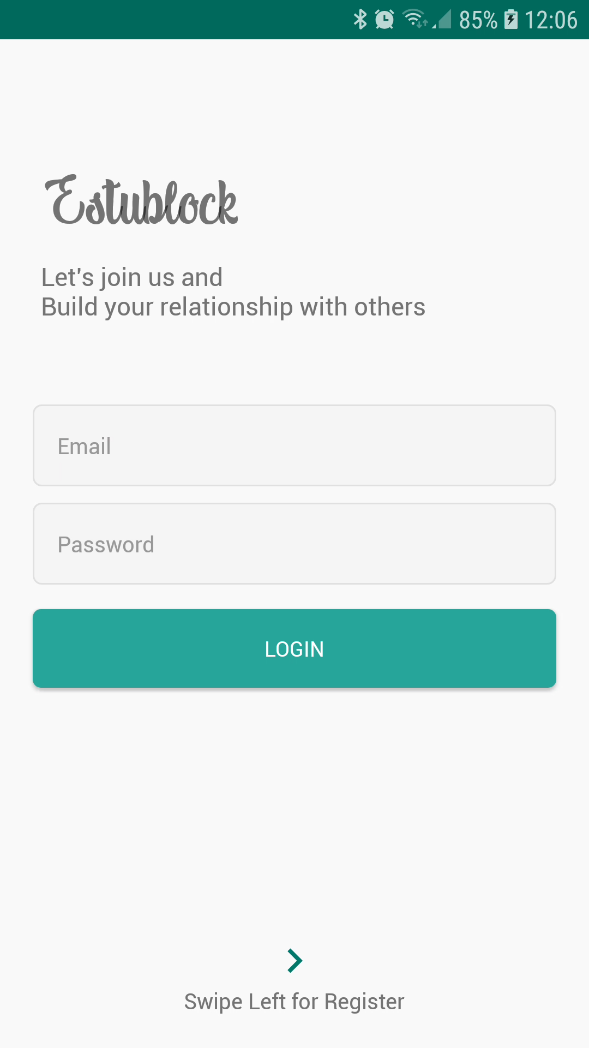
\includegraphics[width=0.7\linewidth]{figs/Desarrollo/Interfaz/estublock_login}
        \caption[Estublock Login]{Pantalla de login de Estublock}
	\end{subfigure} 
	\caption[Pantalla de Login]{Pantalla de Login}
	\label{fig:pantalla_login}
\end{figure}

\subsubsection{Menú Principal}

El menú principal es el corazón de la aplicación. Pues desde ahí se abre camino al resto de funcionalidades de la aplicación. Por un lado es una pantalla importante, pues recoge gran parte de los componentes de la aplicación, pero a su vez, es muy básica y no tiene nada interesante, pues lo único que hace es redirigir al usuario a las funcionalidades disponibles. Estéticamente hablando, la pantalla que se diseño en Marvelapp ha perdido mucho valor visual, pues la pantalla resultante es más básica y menos colorida. Sin embargo, aunque la estética es importante, la funcionalidad principal del menú es redirigir al usuario y esto sí lo hace perfectamente bien. El diseño final así como los botones han sufrido muchos cambios. De hecho, excepto el botón de \emph{asignaturas} el resto de botones es diferente. Esta decisión se ha tomado para agilizar el objetivo principal de la aplicación, es decir, queremos escanear QRs para validar la asistencia de usuarios a eventos. Por tanto, tenemos un botón \emph{crear eventos}, un botón \emph{asistencia} que genera el QR y un botón \emph{Escanear QR} que permite escanear los QR. Desde el menú se puede hacer todo, los cambios se pueden ver en la figura\ref{fig:pantalla_menu}. \\

\begin{figure}[hbt]
	\centering
	\begin{subfigure}[b]{0.4\linewidth}
		\centering
        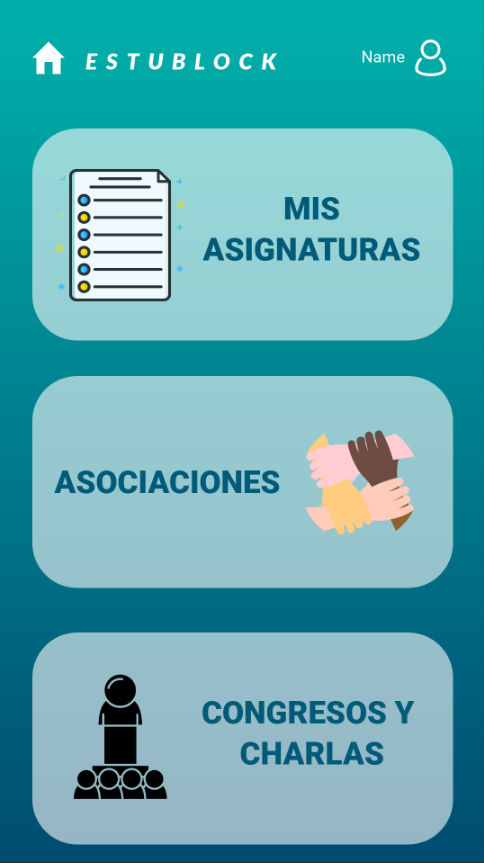
\includegraphics[width=0.7\linewidth]{figs/Desarrollo/Interfaz/marvel_menu}
        \caption[Marvel Menú]{Pantalla de menú de marvelapp}
	\end{subfigure} 
	\begin{subfigure}[b]{0.4\linewidth}
		\centering
        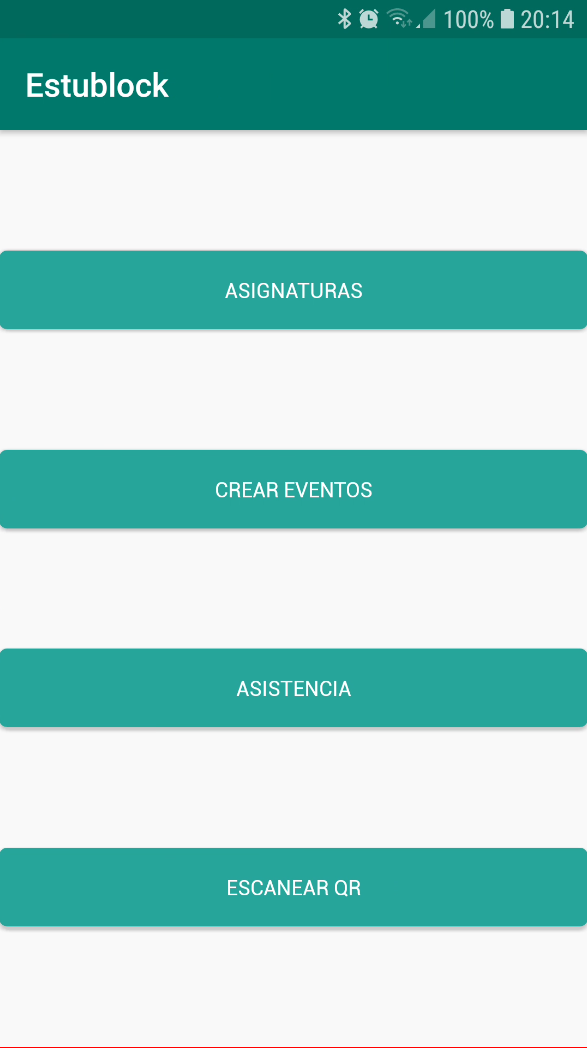
\includegraphics[width=0.7\linewidth]{figs/Desarrollo/Interfaz/estublock_menu}
        \caption[Estublock Menú]{Pantalla de menú de Estublock}
	\end{subfigure} 
	\caption[Pantalla de Menú]{Pantalla de Menú}
	\label{fig:pantalla_menu}
\end{figure}

\subsubsection{Pantalla de Suscripciones}

En la pantalla de suscripciones el usuario puede ver la lista de asignaturas a las que esta suscrito. También se le permite añadir y eliminar asignaturas, para que según avance el curso y vaya aprobando asignaturas pueda no verlas en la lista. Visualmente la pantalla de Marvelapp y la de Estublock han cambiado, pero las funcionalidades. Los que sí se puede destacar, es que se ha puesto en la pantalla de Estublock un botón grande que pone \textit{Añadir} y otro \textit{Eliminar} con esto lo que conseguimos es que el usuario tenga claro donde puede ir a añadir asignaturas o eliminarlas. En la pantalla que se hizo con Marvelapp, el botón de añadir es pequeño y se encuentra en una esquina, y puede no verse con claridad. El diseño de la pantalla queda mostrado en la siguiente figura\ref{fig:pantalla_asignaturas}

\begin{figure}[hbt]
	\centering
	\begin{subfigure}[b]{0.4\linewidth}
		\centering
        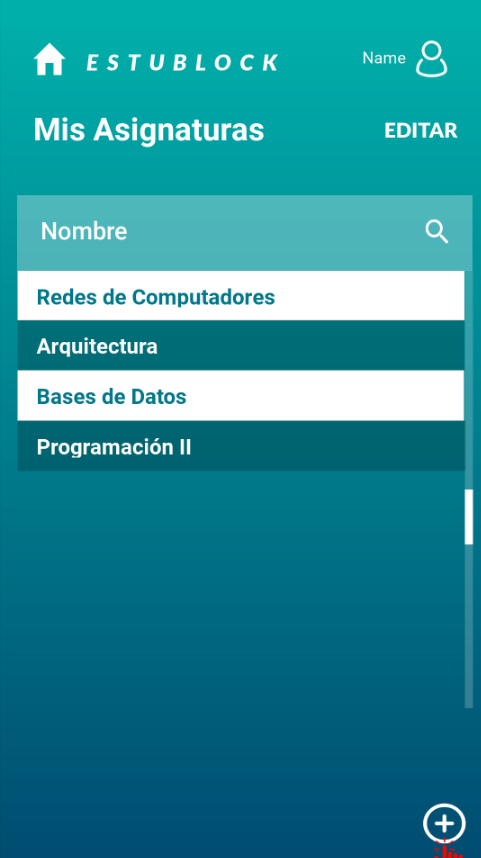
\includegraphics[width=0.7\linewidth]{figs/Desarrollo/Interfaz/marvel_lista_asignaturas}
        \caption[Marvel Asignaturas]{Pantalla de asignaturas de marvelapp}
	\end{subfigure} 
	\begin{subfigure}[b]{0.4\linewidth}
		\centering
        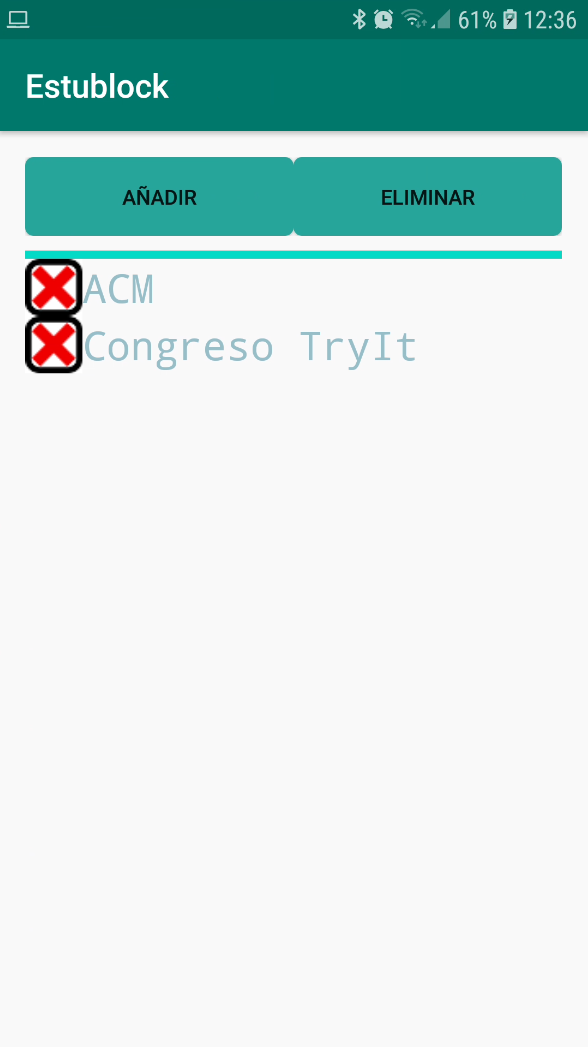
\includegraphics[width=0.7\linewidth]{figs/Desarrollo/Interfaz/estublock_asignaturas_suscritas}
        \caption[Estublock Asignaturas]{Pantalla de asignaturas de Estublock}
	\end{subfigure} 
	\caption[Pantalla de Asignaturas]{Pantalla de Asignaturas}
	\label{fig:pantalla_asignaturas}
\end{figure}

Si el usuario decide añadir nuevas asignaturas a su lista, tendrá que darle al botón de \textit{Añadir}. Esto le lleva a una nueva pantalla en la que se listan todas las asignaturas que hay disponibles para suscribirse. Una vez el usuario selecciona las asignaturas puede proceder a guardarlas. Con respecto al diseño original y al resultado final, caben destacar dos aspectos. El primero es que el botón \textit{Guardar} se ha movido de sitio, no hay ninguna razón especial para esta decisión. Por otro lado, lo que falta es un buscador de asignaturas, este no se ha añadido por ahora, pues no era de crucial importancia al no tener una lista grande de asignaturas disponibles. Sin embrago, es importante que esto se añada en el futuro, pues son muchas las asignaturas que pueden acumularse. El resultado puede verse en \ref{fig:pantalla_añadir_sus}

\begin{figure}[hbt]
	\centering
	\begin{subfigure}[b]{0.4\linewidth}
		\centering
        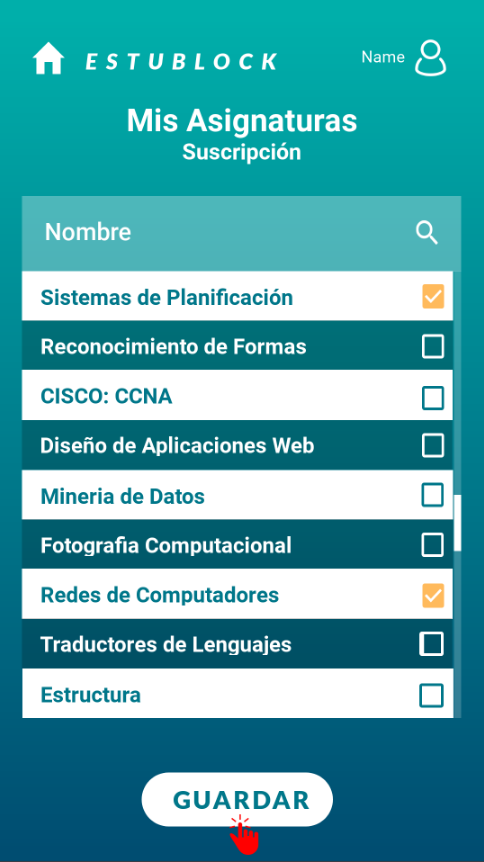
\includegraphics[width=0.7\linewidth]{figs/Desarrollo/Interfaz/marvel_asignaturas}
        \caption[Marvel Suscribirse]{Pantalla de suscripción de marvelapp}
	\end{subfigure} 
	\begin{subfigure}[b]{0.4\linewidth}
		\centering
        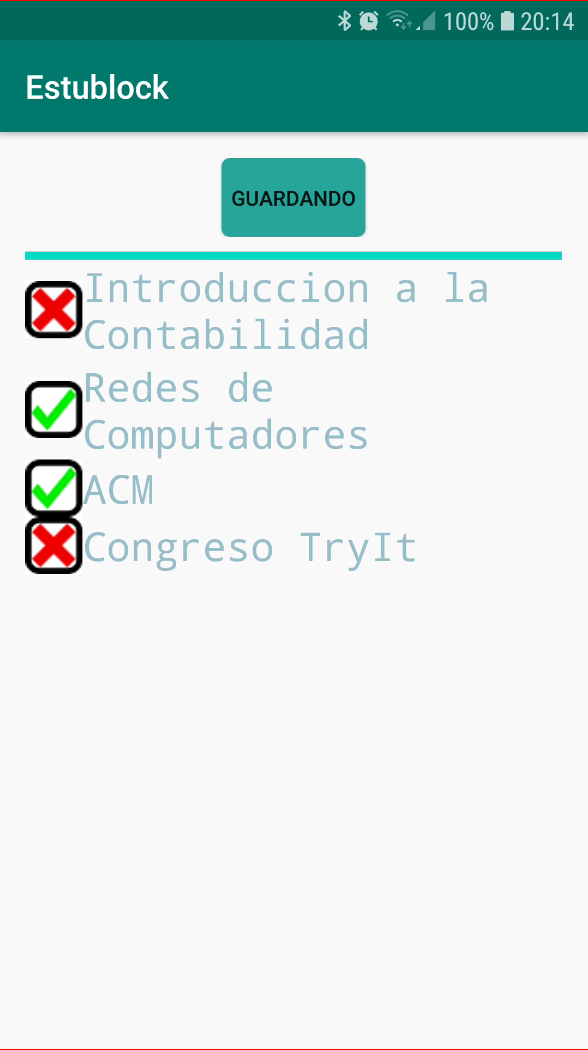
\includegraphics[width=0.7\linewidth]{figs/Desarrollo/Interfaz/estublock_asignaturas}
        \caption[Estublock Suscribirse]{Pantalla de suscripción de Estublock}
	\end{subfigure} 
	\caption[Pantalla de Suscribirse]{Pantalla de Suscribirse}
	\label{fig:pantalla_añadir_sus}
\end{figure}

\subsubsection{Pantalla de Creación de Eventos}

Para llegar a esta pantalla, el usuario tiene que ir desde el menú, a \textit{Crear Evento}, luego se le muestra una pantalla con la lista de asignaturas a las que esta suscrito, y una vez seleccionada la asignatura de la que se quiere crear un evento, se le muestra la pantalla de creación de eventos. En esta pantalla el usuario debe introducir datos sobre el evento como el nombre, fecha, hora, descripción\dots Esta pantalla se ha mantenido muy parecida al diseño realizado con Marvelapp. La única diferencia es que en Marvellapp, el usuario pulsaba \textit{Siguiente} y podía ver un resumen de los datos antes de guardarlos. Se ha decidido eliminar este paso extra, por no aportar nada, pues el usuario puede ver los datos que ha introducido de todos modos en la propia creación del evento, guardando una vez este seguro de los datos elegidos. A continuación se pueden ver unas capturas del resultado \ref{fig:pantalla_crear_evento}, \ref{fig:pantalla_hora}

\begin{figure}[hbt]
	\centering
	\begin{subfigure}[b]{0.4\linewidth}
		\centering
        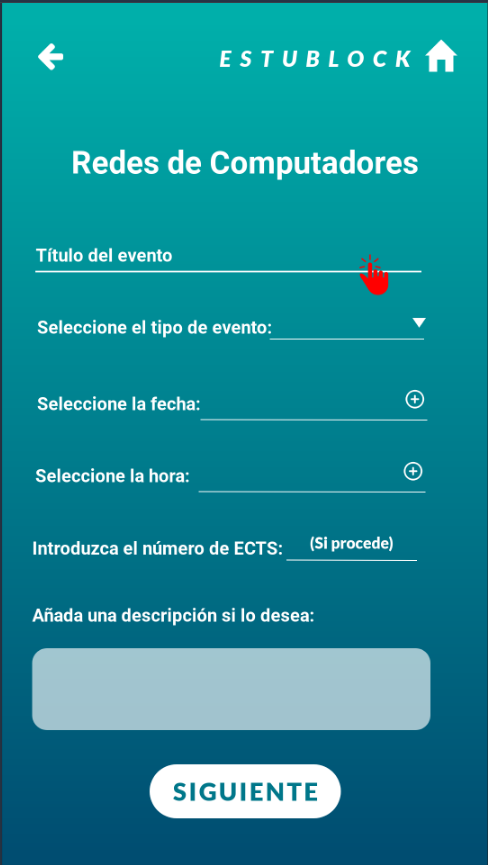
\includegraphics[width=0.7\linewidth]{figs/Desarrollo/Interfaz/marvel_crear_evento}
        \caption[Marvel Crear Evento]{Pantalla de creación de evento de marvelapp}
	\end{subfigure} 
	\begin{subfigure}[b]{0.4\linewidth}
		\centering
        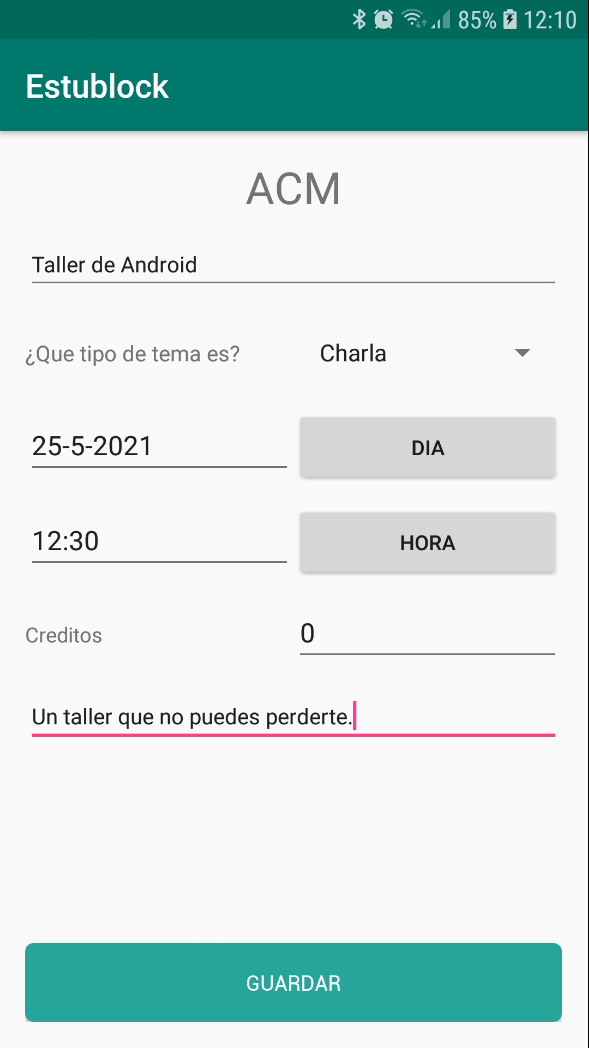
\includegraphics[width=0.7\linewidth]{figs/Desarrollo/Interfaz/estublock_crear_evento_completo.png}
        \caption[Estublock Crear Evento]{Pantalla de creación de evento de Estublock}
	\end{subfigure} 
	\caption[Pantalla de Crear Evento]{Pantalla de Crear Evento}
	\label{fig:pantalla_crear_evento}
\end{figure}

\begin{figure}[hbt]
	\centering
	\begin{subfigure}[b]{0.4\linewidth}
		\centering
        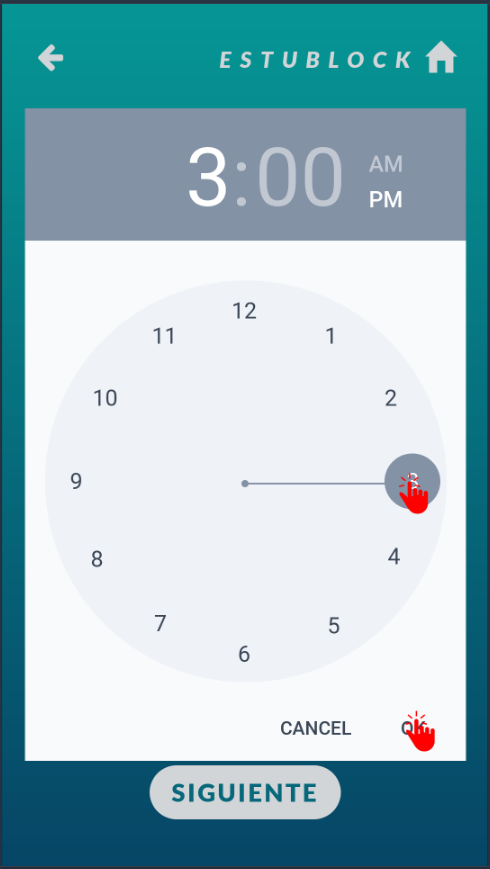
\includegraphics[width=0.7\linewidth]{figs/Desarrollo/Interfaz/marvel_crear_evento_hora}
        \caption[Marvel Hora]{Pantalla de hora de marvelapp}
	\end{subfigure} 
	\begin{subfigure}[b]{0.4\linewidth}
		\centering
        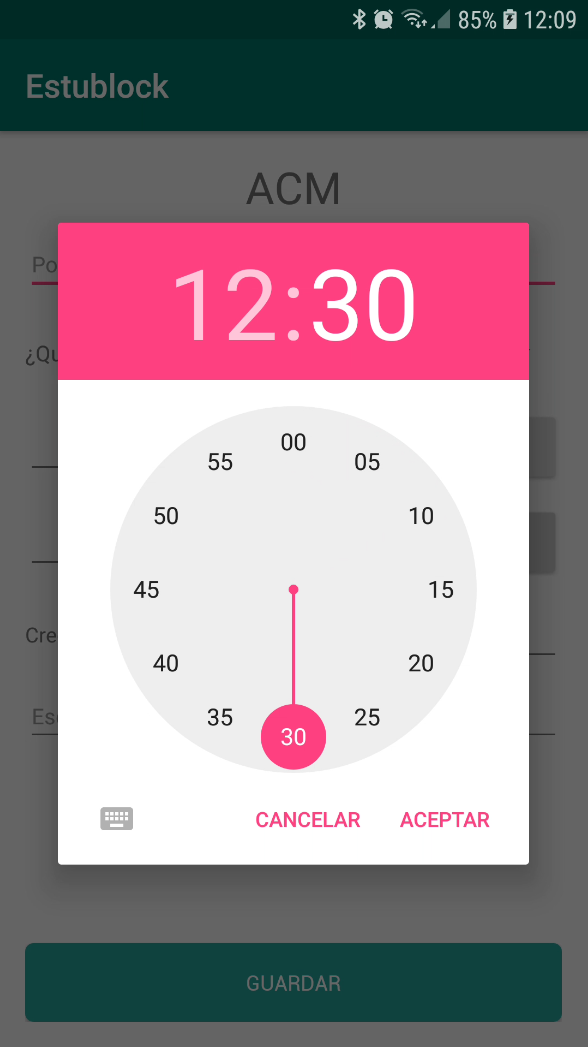
\includegraphics[width=0.7\linewidth]{figs/Desarrollo/Interfaz/estublock_crear_evento_hora}
        \caption[Estublock Hora]{Pantalla de hora de Estublock}
	\end{subfigure} 
	\caption[Pantalla de Hora]{Pantalla de Hora}
	\label{fig:pantalla_hora}
\end{figure}

\subsubsection{Pantalla de generar un QR}

Para llegar a esta pantalla, el usuario ha elegido previamente el botón \textit{Asistencia} así como seleccionar la asignatura y evento al que se quiere registrar. En la pantalla, aparece un gran QR que el profesor debe escanear. Esto es \textbf{muy importante}, es uno de los grandes cambios en la forma en la que se registra la asistencia. Al diseñar la aplicación ``Estublock'' en Marvelapp, se planteó que el profesor enseñaría el QR y los alumnos lo escanearían. Sin embargo ahora se hace al revés. Esta decisión se ha tomado, ya que quien tiene que firmar las transacciones a la red Blockchain es el profesor, para ello, tiene que ser él quien lea los datos de un alumno y firme con su wallet que ese alumno ha asistido al exámen. Luego, la pantalla ha quedado más sencilla, pero con mucho más espacio para él QR y así facilitar su escaneo. La pantalla del QR se puede ver a continuación \ref{fig:pantalla_qr}

\begin{figure}[hbt]
	\centering
	\begin{subfigure}[b]{0.4\linewidth}
		\centering
        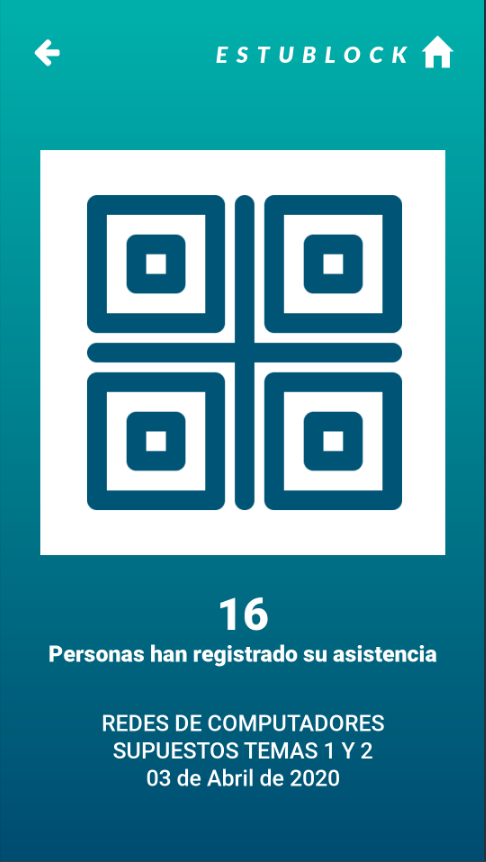
\includegraphics[width=0.7\linewidth]{figs/Desarrollo/Interfaz/marvel_QR}
        \caption[Marvel QR]{Pantalla de QR de marvelapp}
	\end{subfigure} 
	\begin{subfigure}[b]{0.4\linewidth}
		\centering
        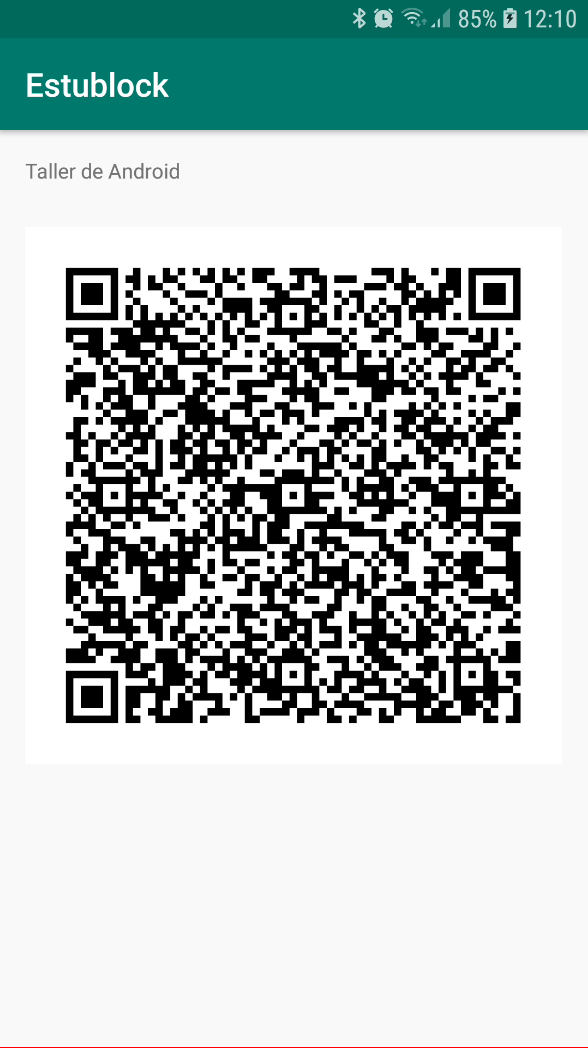
\includegraphics[width=0.7\linewidth]{figs/Desarrollo/Interfaz/estublock_QR}
        \caption[Estublock QR]{Pantalla de QR de Estublock}
	\end{subfigure} 
	\caption[Pantalla de QR]{Pantalla de QR}
	\label{fig:pantalla_qr}
\end{figure}

\subsubsection{Pantalla del Escanear un QR}

Esta pantalla es especial, pues llama a la actividad de la \textbf{cámara de fotos}. Como hemos visto anteriormente en el estado del arte, una aplicación puede llamar sin problemas a otra aplicación (siempre y cuando esta lo permita). En esta ocasión, se requiere de la cámara del usuario para escanear el QR. No todas las cámaras de los móviles escanean QRs de forma automática, pero esto no es un problema ya que la librería que se ha utilizado para programar esta actividad, se encarga de ello. El usuario entonces verá como se abre su cámara y al enfocar un QR, este se escanea automáticamente enviando a la red blockchain la asistencia. Una representación visual puede verse en \ref{fig:pantalla_escaneo_qr}

\begin{figure}[h!]
  \centering
  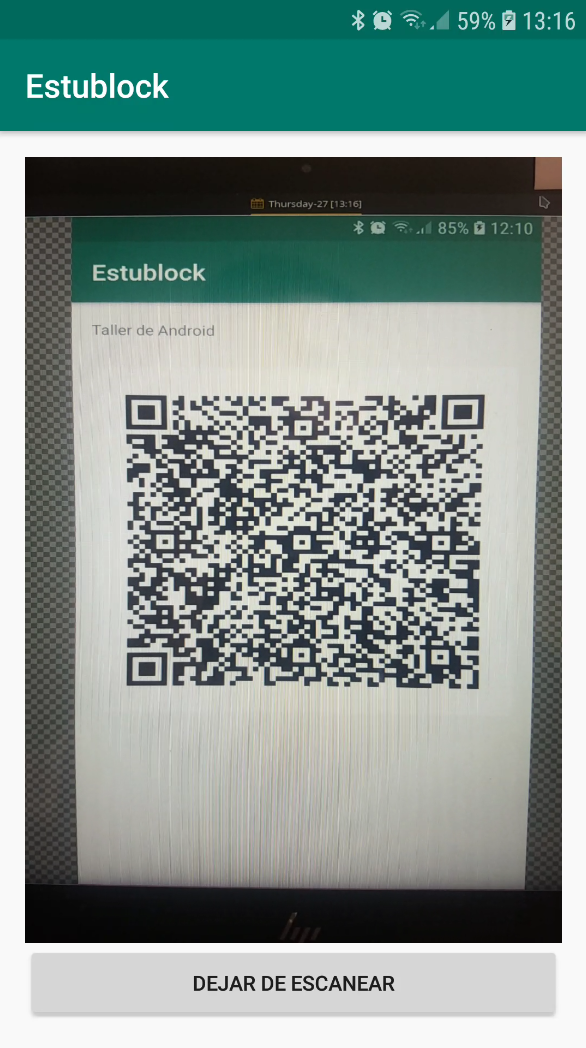
\includegraphics[width=0.3\linewidth]{figs/Desarrollo/Interfaz/estublock_escanear_qr}
  \caption[Pantalla de Escaneo de QR]{Pantalla de escaneo de QR Estublock}
  \label{fig:pantalla_escaneo_qr}
\end{figure}

% --------------------------------------------------
\subsection{Implementación XML}

Como ya hemos mencionado, las interfaces de usuario en Android se programan utilizando código XML. XML, del ingles \emph{Extensible Markup Language} es un metalenguaje que permite definir con un lenguaje de marcas información y datos. Es parecido a HTML, pero las etiquetas no estan predefinidas sino que puedes inventarte las que quieras. Permite crear estructuras con parámetros y atributos los cuales pueden utilizarse por ejemplo en internet para enviar datos a una API. En el caso de las aplicaciones móvil, el código XML se utiliza para diseñar las pantallas o \emph{layouts}, ya que XML es un lenguaje ligero y esto hace que las pantallas sean ligeras también. Es con el código XML con el que se definen las jerarquías que se mencionan en el apartado \hyperref[sec:GUI]{3.2.1}, por ejemplo, parte de la estructura de la pantalla \emph{crear un evento} puede verse en \ref{fig:xml_crear_evento} se han omitido los atributos para ahorrar espacio. 

\begin{figure}[h!]
  \centering
  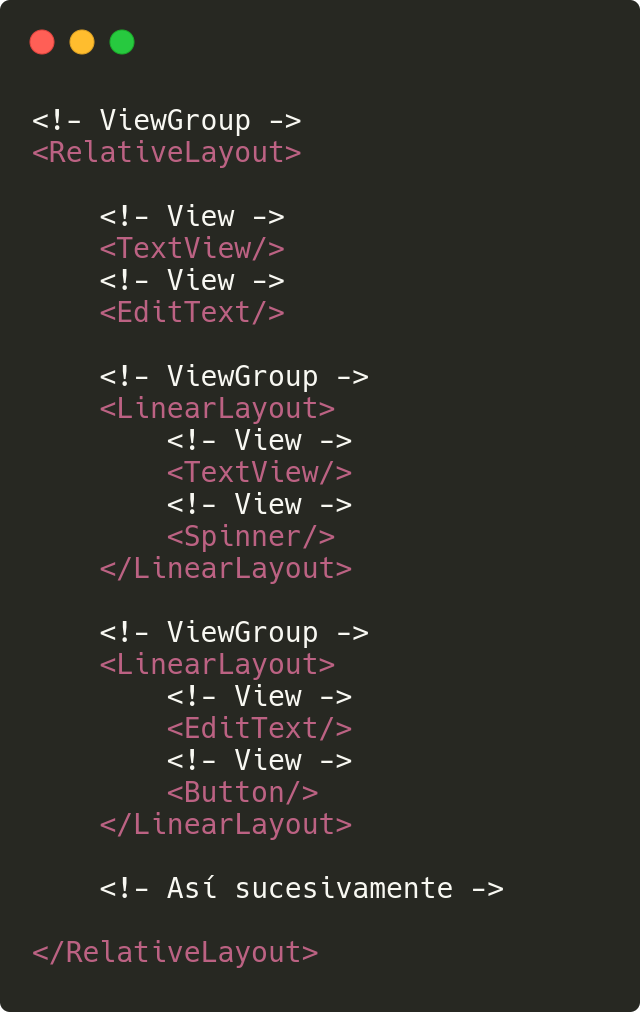
\includegraphics[width=0.5\linewidth]{figs/Desarrollo/Codigo/xml_jerarquia}
  \caption[XML Jerarquia]{Fragmento de la jerarquía XML de la pantalla crear evento}
  \label{fig:xml_crear_evento}
\end{figure}

Programar pantallas para Android sin ningún tipo de feedback, es decir, sin saber como esta quedando la pantalla, es muy difícil. Por eso, Android Studio, trae consigo una herramienta de gran utilidad, la que cual permite visualizar y editar el código sin tener que escribirlo por completo. Se puede por ejemplo crear un botón, y la herramienta de forma automática escribirá el código XML correspondiente, luego se puede cambiar el color del botón, y la herramienta se encargará de escribir el código XML correspondiente. Sin embargo, tras una actualización de Android Studio (actualización a la versión 4.2.0.24-1) el sistema de atributos dejó de funcionar, y hubo que añadir los atributos manualmente, esto supuso un tiempo extra a la hora de realizar las pantallas, y es una de las razones por las que las pantallas (excepto login y registro) han quedado visualmente más básicas. La herramienta de Android Studio puede encontrarse en la figura\ref{fig:herramienta_android}.

\begin{figure}[h!]
  \centering
  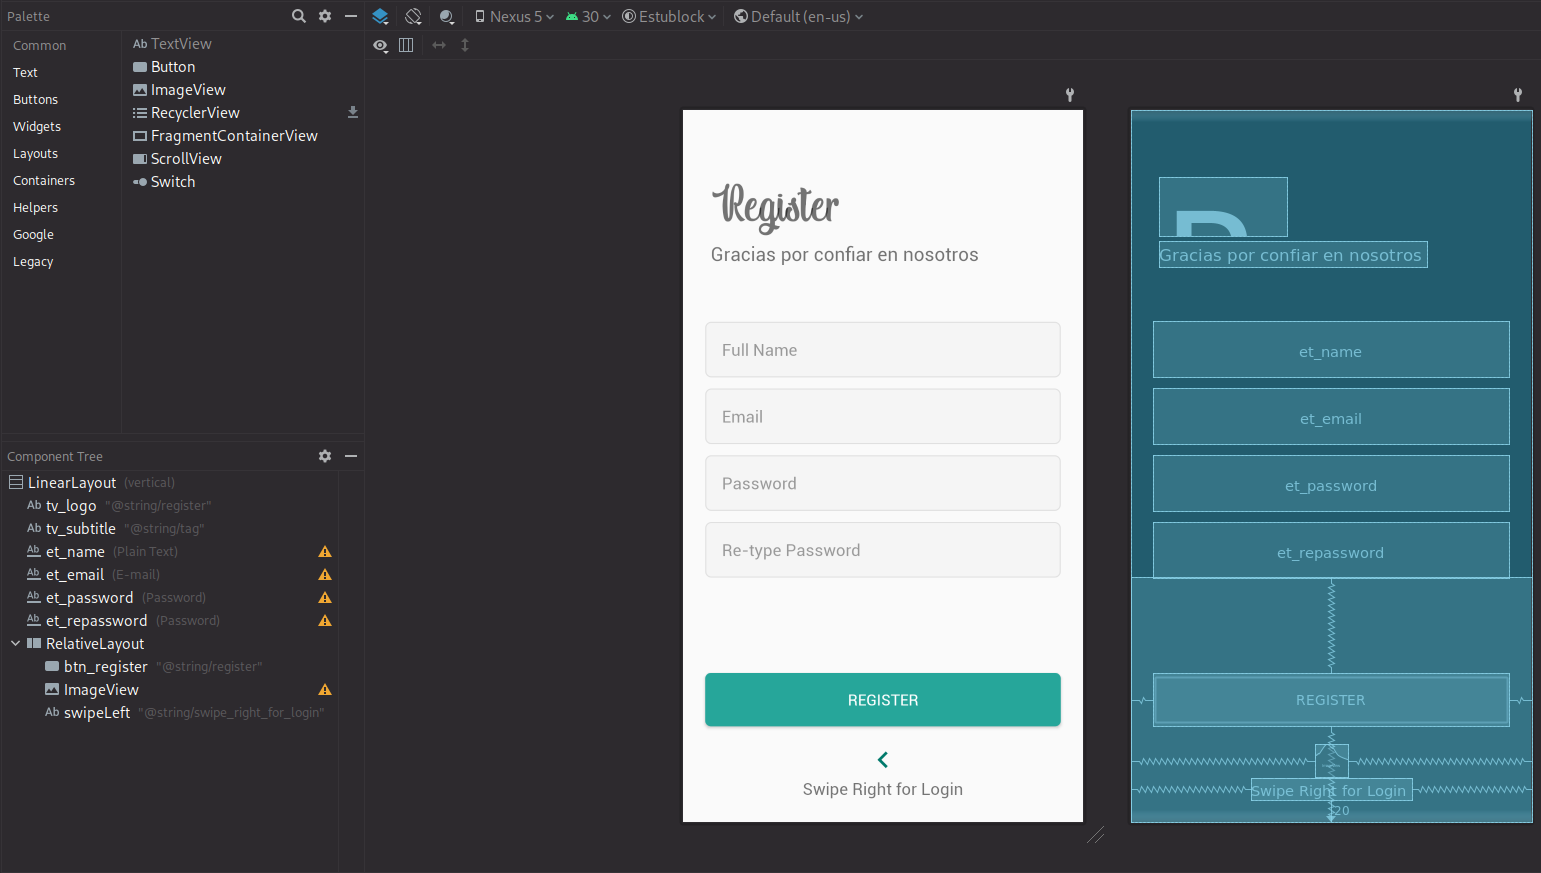
\includegraphics[width=1\linewidth]{figs/Desarrollo/XML/androidStudio}
  \caption[XML Herramienta Android Studio]{Herramienta de Android Studio para la edición de layouts (pantallas)}
  \label{fig:herramienta_android}
\end{figure}

XML no solo sirve para diseñar las pantallas, hasta ahora todo lo que hemos comentado se refería al esqueleto de una pantalla. Es decir, un botón arriba, un texto pegado abajo a la derecha\dots Pero con XML también se puede modificar la apariencia, color, forma, fuente de todos los elementos. Dentro de las carpetas de un proyecto Android, tenemos algunas carpetas en las que se guarda código XML que se utiliza posteriormente para darle un mejor diseño a un elemento. Por ejemplo, se puede crear un botón y asignarle un fondo con el atributo \textit{android:background} a este atributo se le añade como parámetro la ruta al archivo que contiene la información en XML sobre como queremos que se vea este botón. Por otro lado, hemos mencionado también las fuentes, los archivos que modifican las fuentes son de tipo \emph{TrueType Font} y definen la fuente de las letras. Por ejemplo, si creamos un campo de texto \textit{TextView} podemos ponerle una fuente especifica con el atributo \textit{android:fontFamily}. Básicamente, somos libres de modificar con total control cada aspecto que se quiera de las pantallas. \\

Por último, haremos mención de una carpeta muy importante llamada \textbf{values} en la que se guardan parámetros para definir los colores, las dimensiones de la pantalla, los distintos temas disponibles y un archivo llamado \textbf{strings} el cual guarda todo el texto estático que se quiere añadir a las pantallas. Este archivo existe, para facilitar el migrado de la aplicación a otros idiomas. Por ejemplo, en vez de escribir en un \textit{TextView} una palabra en español, se le asignará un identificador dentro del archivo \emph{strings}, de modo que si alguna vez tenemos varios idiomas disponibles, se puede tener con el mismo identificador la palabra en varios idiomas, y será tan sencillo como decirle a Android que utilice un archivo \emph{strings} u otro, de modo que las pantallas no hay que modificarlas nunca si se quiere cambiar de idioma. Lo mismo aplica a los colores, temas (si queremos un tema oscuro, no hay que cambiar las pantallas sino que se cambian los colores del archivo de temas y el archivo de colores)\dots Básicamente, aportan flexibilidad y escalabilidad en la aplicación para poder modificarla con más seguridad y rapidez. 




% --------------------------------------------------
\section{Implementación} \label{sec:Codigo}

Las aplicaciones Android pueden ser programadas principalmente en dos lenguajes de programación, \textbf{Java} y \textbf{Kotlin}. En el presente, la inmensa mayoría de aplicaciones han sido desarrolladas con Java, sin embargo Kotlin es promete ser el futuro. Actualmente sigue siendo un lenguaje muy secundario (aunque se puede hacer todo lo que se puede hacer con Java y esta muy bien documentado). Según google trends\ref{fig:java_vs_kotlin}, Kotlin esta lejos de quitarle el puesto a Java aunque los nuevos desarrolladores de aplicaciones Android muestran más interés por Kotlin por su comodidad, falta de verbosidad y ``limpieza'' (es decir, con menos líneas de código haces lo mismo que Java). 

\begin{figure}[h!]
  \centering
  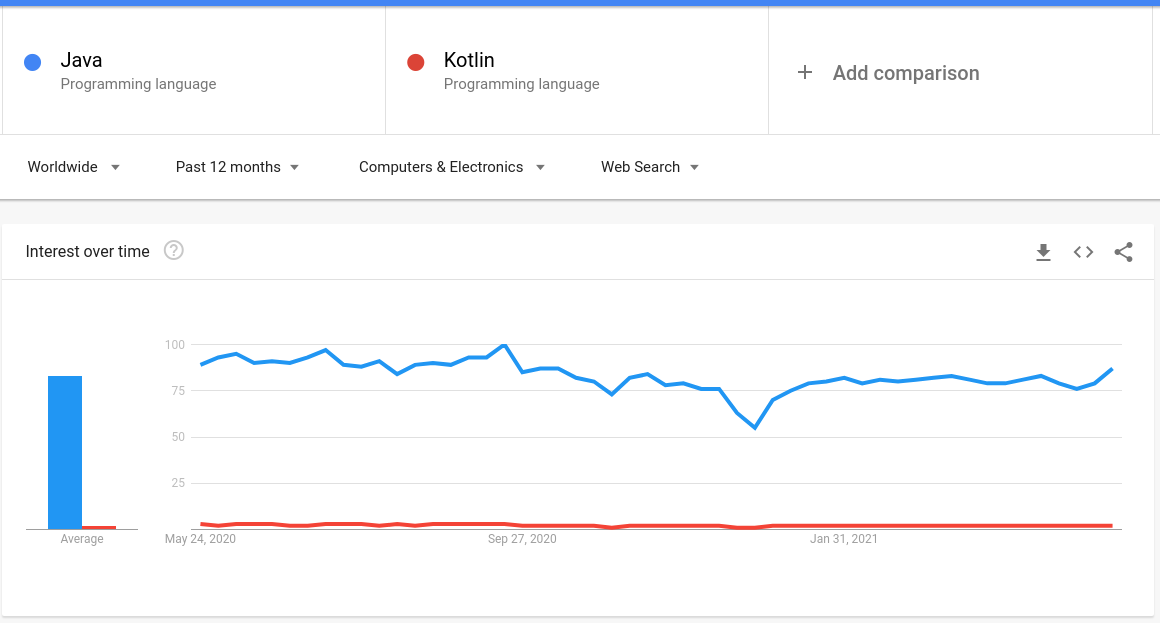
\includegraphics[width=0.9\linewidth]{figs/Desarrollo/Popularidad}
  \caption[Java vs Kotlin]{Comparación de Google Trends entre Java y kotlin}
  \label{fig:java_vs_kotlin}
\end{figure}

Por lo tanto, aunque Kotlin promete mucho, la aplicación Estublock se ha desarrollado en el lenguaje Java para tener una mayor cantidad de documentación y de comunidad disponible. Con comunidad, nos referimos a las personas en el planeta que saben de programación Android con Java y que a lo largo de los años han respondido y contribuido en Internet, dando soluciones a problemas, documentación y contando sus trucos profesionales. De todos modos, se puede migrar con mucha facilidad a Kotlin puesto que AndroidStudio permite migrar automáticamente de Java a Kotlin. Lo único que se necesita para facilitar este proceso es añadir ``anotaciones de java'' que especifiquen las características de algunas variables o funciones para facilitar a AndroidStudio el reconocimiento de las variables. Un ejemplo puede encontrarse a continuación \ref{fig:nonNull} donde se puede ver que se especifica que la variable no puede ser nula con \emph{@NonNull}.

% \begin{lstlisting}[language=Java,float=ht,caption={[Java] Ejemplo de ``anotación de java'' de variables para facilitar el salto a Kotlin},label=lst:java_etiquetas]
% public void sendSignedTransaction(@NonNull String signedMessage){
%   // Código
% }
% \end{lstlisting}

\begin{figure}[h!]
  \centering
  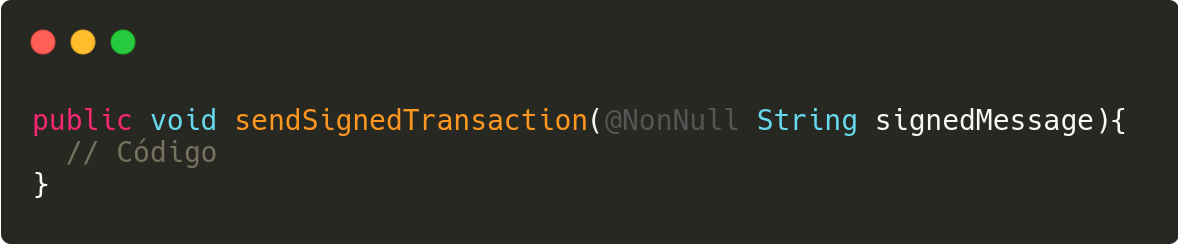
\includegraphics[width=0.9\linewidth]{figs/Desarrollo/nonNull}
  \caption[Facilitar el salto a Kotlin]{Ejemplo de anotación de java de variables para facilitar el salto a Kotlin}
  \label{fig:nonNull}
\end{figure}


% --------------------------------------------------
\subsection{Implementación Java}

Todo el código de la aplicación esta disponible en mi repositorio de github\cite{forgis98}. Vamos a tratar de resumir el trabajo realizado, pues gran parte de este TFG esta reflejado en la aplicación móvil que se ha desarrollado. \\

\subsubsection{Archivos del Proyecto}

% Manifest XML
% Gradle
% Estructura de Estublock
% Estructura del SDK

Un proyecto en Android Studio dispone de un gran conjunto de carpetas y archivos que hacen funcionar a la aplicación entera. En el caso de ``Estublock'' vamos a mencionar los que son de gran importancia. Empezando por \textbf{AndroidManifest.xml}, todos los proyectos Android deben tener un archivo con este nombre en la raíz del proyecto. Este archivo, describe información esencial de la aplicación para las herramientas de creación de Android y para el sistema operativo. Entre otras cosas, el archivo declara el nombre del paquete que contiene la aplicación, los componentes de la aplicación (actividades, servicios\dots), los permisos de los que requiere la aplicación como permiso a la cámara o a internet como en el caso de ``Estublock''. Si se usa Android Studio, este archivo se creará automáticamente pero para añadir permisos ha de hacerse manualmente. En el proyecto ``Estublock'' se han añadido a este archivo los permisos de acceso a \textbf{Internet}, escritura de \textbf{datos en memoria} y a la \textbf{cámara} del dispositivo. \\

Por otro lado, toda una carpeta de gran importancia en el proyecto es la carpeta de \textbf{Gradle}. Gradle es un paquete de herramientas de compilación avanzadas, que permite automatizar y administrar el proceso de compilación. Al ser una herramienta de compilación, trae consigo un conjunto de carpetas y archivos que utiliza para gestionar el proyecto, en concreto esta el archivo \textbf{build.gradle} en el que se escriben las dependencias del proyecto para poder utilizar librerías no incluidas por defecto en java o Android. A la hora de desarrollar la aplicación, se han añadido varias librería que se verán en mejor detalle en \hyperref[sec:librerias]{Librerías} como \textbf{okhttp, bcrypt, web3j}\dots \\

La estructura de carpetas del SDK, es muy parecida a la de ``Estublock'' con la principal diferencia de que no tiene ninguna carpeta de interfaz (no tiene carpetas de colores, temas, strings, layouts\dots). Sin embargo tiene su propio archivo \emph{build.gradle} y su propio archivo \emph{AndroidManifest.xml}. Puesto que no tienen grandes diferencias, mostramos solo la estructura de la carpeta que contiene el proyecto ``Estublock'' pues tiene más contenido que el SDK \ref{fig:jerarquia_estublock} \\

\begin{figure}[h!]
  \centering
  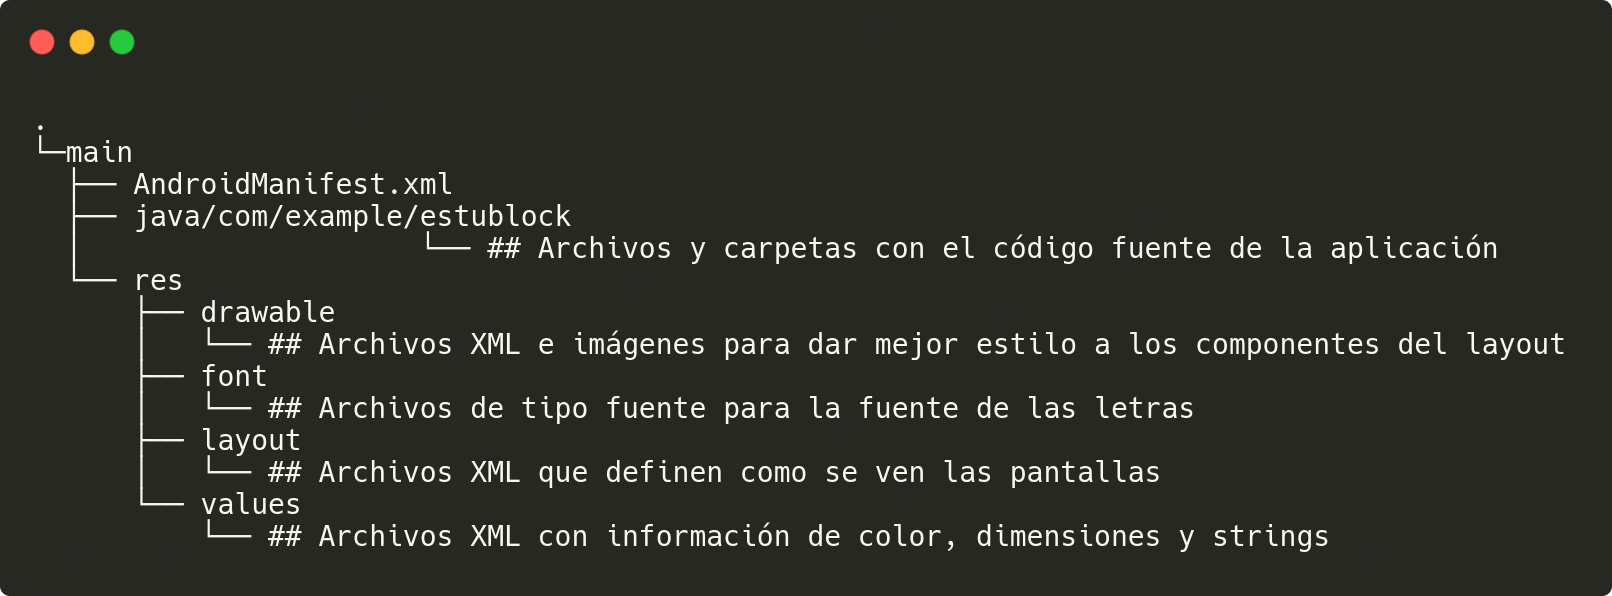
\includegraphics[width=0.9\linewidth]{figs/Desarrollo/JerarquiaCarpetas}
  \caption[Jerarquia Estublock]{Jerarquia de carpetas del proyecto Estublock}
  \label{fig:jerarquia_estublock}
\end{figure}

Por último, al ejecutar la aplicación en el dispositivo móvil por primera vez y registrar a un usuario, se crea en el directorio de carpetas del usuario dos archivos nuevos. Uno de ellos es el \hyperref[sec:wallet]{wallet} del cual hablaremos más adelantes. Y el otro es una carpeta con un archivo en el que guardar datos en forma de un par \{claves $->$ valor\}. Este carpeta se llama \textbf{shared preferences}. En el caso de la aplicación, se utiliza para guardar el directorio en el que se ha guardado el wallet.

\subsubsection{Librerías utilizadas} \label{sec:librerias}

Se han utilizado 8 librerías extras (a parte de las que incluye por defecto android al iniciar el proyecto). \emph{web3j} se mencionará en el apartado del \hyperref[sec:SDK]{SDK} y \emph{play-services-vision} es necesaria para \emph{ZXing} pero no se ha usado directamente. Queda entonces: \\
\begin{enumerate}
\item \textbf{Volley: } Volley es una biblioteca HTTP que facilita y agiliza el uso de redes en apps para Android. Permite programación automática de solicitudes de res, varias conexiones de red simultáneas, almacenamiento de respuestas en cache\dots Se ha utilizado esta librería para todas las llamadas excepto la llamadas \emph{DELETE} ya que daba problemas. Algo muy interesante de Volley es que las llamadas son asíncronas, es decir, se ejecutan separadas del hilo principal no bloqueándolo y una vez se recibe la respuesta de la llamada se puede recuperar la información en un callback. Un ejemplo de llamada POST puede verse en \ref{fig:post_volley} \\

% \begin{lstlisting}[language=Java,float=ht,caption={[Java] Ejemplo de llamada POST con Volley.},label=lst:volley]
% JsonObjectRequest jsonObjectRequest = new JsonObjectRequest(Request.Method.POST,
%     (URL), parametrosJSON,
%     new Response.Listener<JSONObject>() {
%       @Override
%       public void onResponse(JSONObject response) {
%         // Hacer algo con respuesta correcta.
%       }
%     }, new Response.ErrorListener() {
%   @Override
%   public void onErrorResponse(VolleyError error) {
%     // Hacer algo con respuesta error.
%   }
% });
% \end{lstlisting}

\begin{figure}[h!]
  \centering
  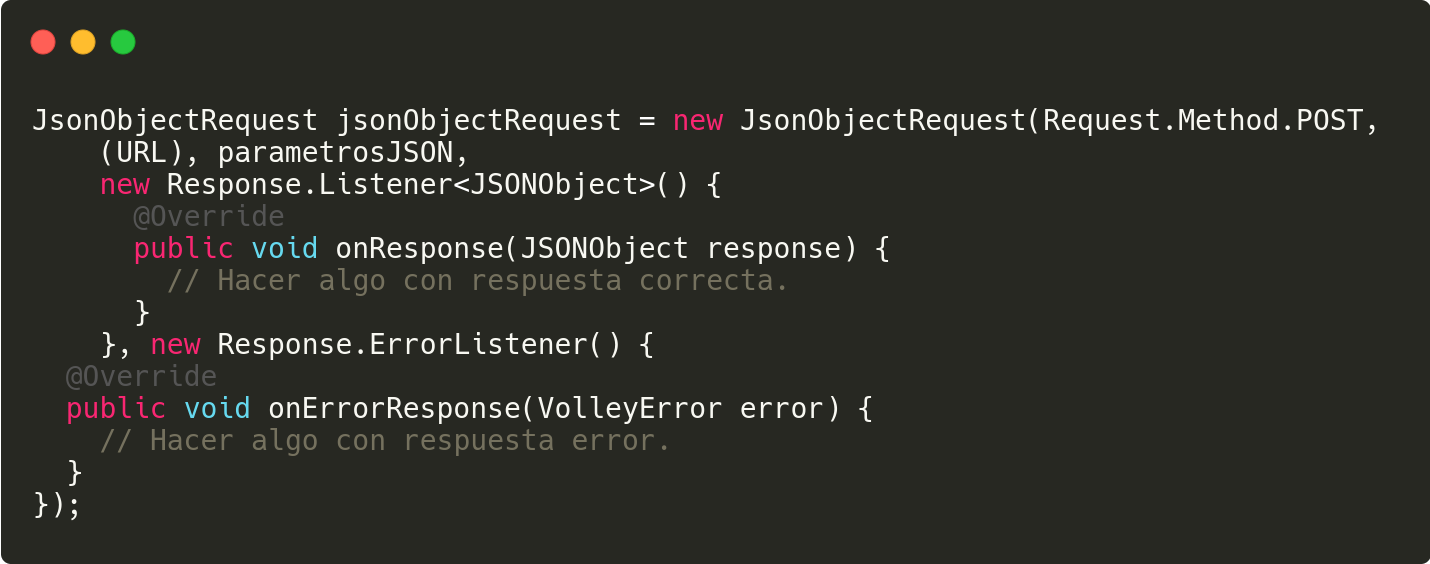
\includegraphics[width=0.8\linewidth]{figs/Desarrollo/Codigo/POST_Volley}
  \caption[Llamada POST con Volley]{Ejemplo de llamada POST con Volley}
  \label{fig:post_volley}
\end{figure}

Para solventar el problema con la llamada DELETE se ha usado la librería Okhttp.

\item \textbf{Okhttp: } Esta librería cumple la misma función que Volley, permitiendo conexiones HTTP\dots Sin embargo, Volley es asíncrono. Okhttp no lo es, ``obligando'' al programador a hacer las llamadas dentro de un hilo de ejecución nuevo. Un ejemplo se provee en la figura \ref{fig:delete_okhttp}

% \begin{lstlisting}[language=Java,float=ht,caption={[Java] Ejemplo de llamada DELETE con OkHttp.},label=lst:okhttp]
% new Thread(new Runnable() {
%   @Override
%   public void run() {
%     try{
%       // Hacer cosas dentro del Thread
% 
%       okhttp3.RequestBody body = okhttp3.RequestBody.create(
%         paramsJSON.toString(), 
%         MediaType.parse("application/json; charset=utf-8")
%       );
% 
%       okhttp3.Request request = new okhttp3.Request.Builder()
%         .url(URL)
%         .delete(body)
%         .build();
%       okhttp3.Response response = client.newCall(request).execute();
% 
%     } catch(Exception e){
%       // Hacer cosas en caso de error.
%     }
%   }
% }).start();
% \end{lstlisting}

\begin{figure}[h!]
  \centering
  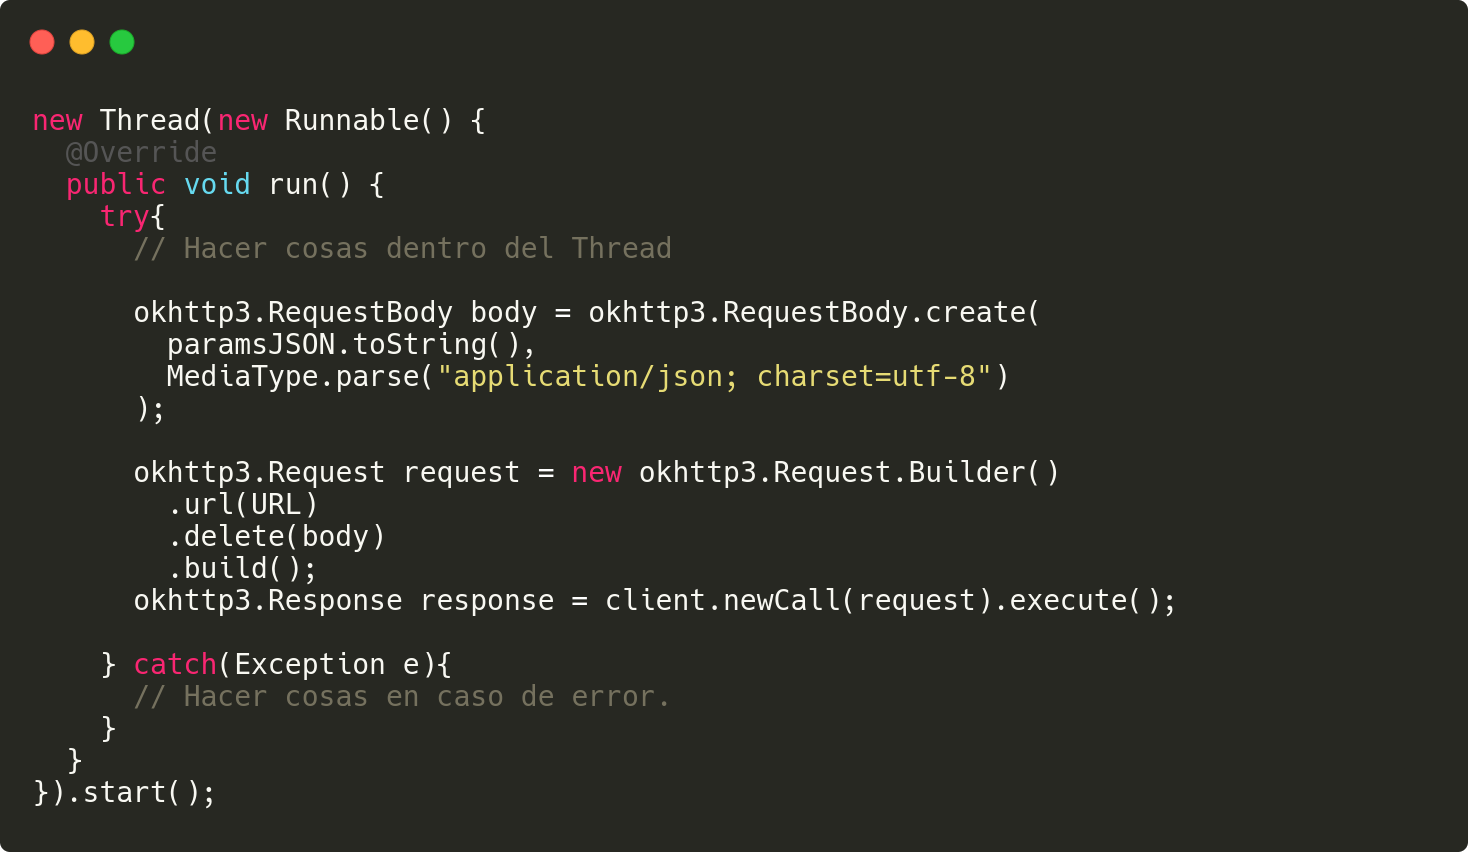
\includegraphics[width=0.8\linewidth]{figs/Desarrollo/Codigo/okhttp_ejemplo}
  \caption[Llamada DELETE con Okhttp]{Ejemplo de llamada DELETE con OkHttp}
  \label{fig:delete_okhttp}
\end{figure}

\item \textbf{Bcrypt: } Es una implementación del algoritmo de hash de contraseñas Blowfish. Básicamente permite cifrar contraseñas para poder guardarlas de forma segura en una base de datos. Con esta librería se cifra la contraseña del usuario que luego se manda a la API para que la guarde en la base de datos como se puede ver en \ref{fig:bcrypt}

% \begin{lstlisting}[language=Java,float=ht,caption={[Java] Ejemplo de cifrado de la contraseña de un usuario.},label=lst:okhttp]
% protected String hashPassword(String password){
%   return BCrypt.withDefaults().hashToString(10, password.toCharArray());
% }
% \end{lstlisting}

\begin{figure}[h!]
  \centering
  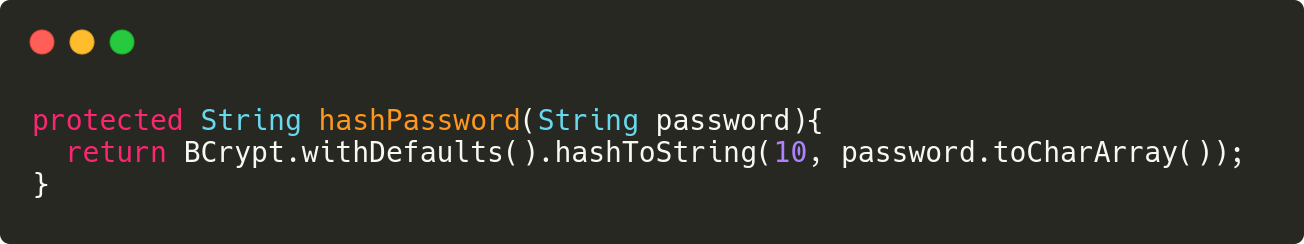
\includegraphics[width=0.8\linewidth]{figs/Desarrollo/Codigo/bcrypt}
  \caption[Ejemplo de cifrado de contraseñas]{Ejemplo de cifrado de la contraseña del usuario}
  \label{fig:bcrypt}
\end{figure}


\item \textbf{QRGenerator: } Librería para generar códigos QR tanto 1D (códigos de barra) como 2D (QR tradicional) con diferentes formatos. Vease \ref{fig:generador_qr}

% \begin{lstlisting}[language=Java,float=ht,caption={[Java] Ejemplo de Código QR},label=lst:okhttp]
% WindowManager manager = (WindowManager) getSystemService(WINDOW_SERVICE);
% Display display = manager.getDefaultDisplay();
% Point point = new Point();
% display.getSize(point);
% 
% qrgEncoder = new QRGEncoder(evento.toString(), null, QRGContents.Type.TEXT, Math.min(point.x, point.y));
% bitmap = qrgEncoder.getBitmap();
% // qr es el identificador de la interfaz de usuario para poner el QR
% qr.setImageBitmap(bitmap);
% \end{lstlisting}

\begin{figure}[h!]
  \centering
  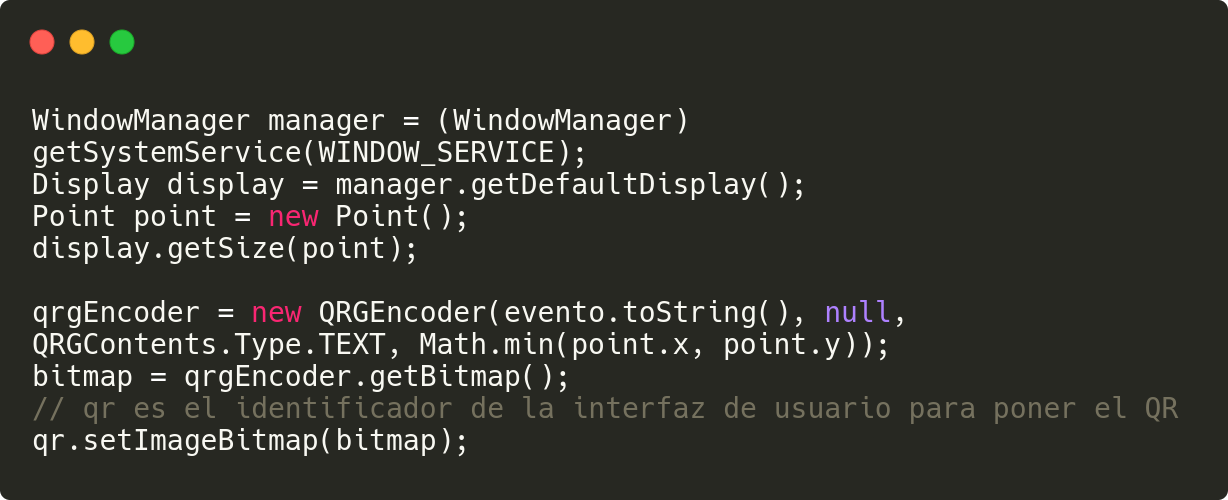
\includegraphics[width=0.8\linewidth]{figs/Desarrollo/Codigo/generador_QR}
  \caption[Ejemplo básico de generar QR]{Ejemplo básico de código de generar QR}
  \label{fig:generador_qr}
\end{figure}

\item \textbf{ZXing: } Esta librería permite generar códigos QR, pero más importante y la razón por la que se ha usado, permite escanear códigos QR. Para generar QR se utilizó la librería anterior puesto que su uso es más fácil de utilizar que ZXing para Android. El código en este caso es bastante más largo por lo que se ha incluido en el \hyperref[cap:Anexo]{Anexo} en concreto en \ref{fig:escaneandoQRs}.

\end{enumerate}

\subsubsection{Archivo GlobalState}

Todos los archivos de código fuente son muy importantes, pues engloban toda la funcionalidad de la aplicación. A la hora de desarrollar aplicaciones, en ocasiones hay que tener en cuenta la información que se quiere guardar sobre el usuario que ha hecho login temporalmente (en ejecución). Una forma de pasar información de una pantalla a otra para mantener por ejemplo el correo de un usuario y poder usarlo en otras pantallas sin tener que volver a pedírselo es utilizando los \emph{Intents}. Un Intent es una descripción abstracta de una operación a realizar, puede utilizarse para lanzar otras actividades y junto al lanzamiento pasar como parámetros valores como se puede ver en \ref{fig:intents} \\

\begin{figure}[h!]
  \centering
  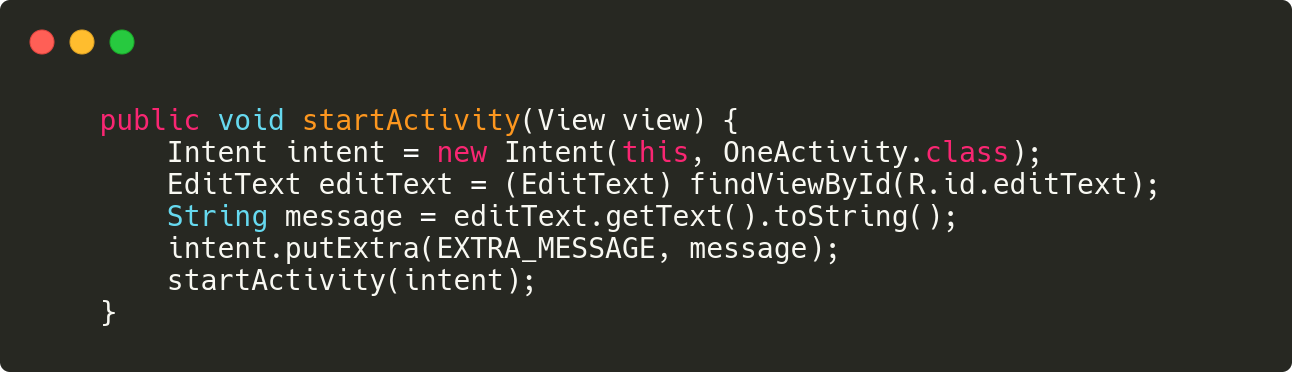
\includegraphics[width=0.8\linewidth]{figs/Desarrollo/Codigo/intents}
  \caption[Ejemplo de Intent en Android]{Ejemplo de Intent en Android}
  \label{fig:intents}
\end{figure}

Sin embargo esto trae una desventaja, siempre que se pase de una a otra pantalla hay que añadir los datos que se quieren guardar para no perderlos, esto puede hacer que si quieres un dato en muchas pantallas, acabes acumulando datos, y hace que el código sea menos legible. Por lo tanto, se tomó la decisión de crear un archivo especial llamado \textbf{GlobalState.java}. Este archivo no tiene una actividad (pantalla) correspondiente, pues su único propósito es el de guardar el estado de algunos datos para evitar pedírselos nuevamente al usuario. Datos como el correo, nombre, directorio donde esta el wallet\dots Pero también se ha aprovechado para guardar las URL de las APIs, nodo de la blockchain\dots El código de este archivo esta disponible en el Anexo ref{fig:gs}



% ##################################################
% ##################################################
\section{SDK} \label{sec:SDK}

Un \emph{Kit de Desarrollo Software} o SDK (Software Development Kit) es generalmente un conjunto de herramientas de desarrollo de software que permiten a otros desarrolladores crear aplicaciones de forma más cómoda. Un buen ejemplo de SDK que se ha utilizado en este proyecto es la familia de SDKs de Android. Junto con AndroidStudio, se instalan múltiples SDKs que permiten al programador escribir código, recuperar componentes de las pantallas, hacer llamadas a paquetes, importar paquetes, detectar errores\dots Todo de forma automática haciendo que la programación sea mucho más fácil. \\

El SDK es entonces un conjunto de métodos los cuales pueden hacer llamadas a una API, llamadas al propio sistema operativo, llamadas a otras librería o SDKs\dots En el caso del SDK desarrollado para este TFG, su principal función es la de hacer llamadas a una red blockchain y la de hacer llamadas al sistema de archivos del dispositivo para guardar el wallet del usuario. 

% --------------------------------------------------
\subsection{Diseño del SDK}

El SDK dispone de 3 archivos separados del proyecto Estublock. Se han creado como librería desde AndroidStudio para poder compartirla después públicamente y que otros programadores puedan utilizarla. Se ha dividido en 3 archivos para tratar de mantener una coherencia entre las funcionalidades que ofrece el SDK. Uno de los archivos se encarga únicamente de gestionar las transacciones, otro archivo se encarga únicamente de gestionar el wallet del usuario, y por último un archivo que se encarga de gestionar los callbacks de las llamadas a la red blockchain, pues estas se ejecutan de manera asíncrona. \\

Por otro lado, con respecto al diseño de los métodos, se ha optado por tratar de programarlos de la forma más genérica posible para que puedan aplicarse en una amplia variedad de situaciones, además se han sobrecargado los métodos (más adelante veremos que significa sobrecargar métodos) para que se puedan utilizar distintos tipos de variables en las funciones sin problema. 

% --------------------------------------------------
\subsection{Comunicación con la Red Blockchain}

En el archivo \emph{TransactionsHelper.java} se encuentra importada la librería de \emph{web3j} y se encuentra también el código que firma y envía las transacciones. Web3j es una biblioteca de Java y Android que permite trabajar con smart contracts e integrarse con clientes o nodos en la red de \emph{Ethereum}. Esto permite trabajar con la red de Ethereum sin necesidad de implementar el código de integración para la plataforma. Implementa la API de cliente JSON-RPC de Ethereum sobre HTTP, soporta wallets, firmado de transacciones\dots JSON-RPC es un protocolo de llamada a procedimientos remotos que utiliza JSON para codificar los mensajes, es similar a XML-RPC. \\

El uso de \emph{TransactionsHelper} es sencillo, primero se crea el objeto pasándole como parámetro la URL del nodo de la red blockchain al que vamos a conectarnos \ref{fig:transH}
% \begin{lstlisting}[language=Java,float=ht,caption={[Java] Constructor de TransactionsHelper},label=lst:constructor]
% // Constructor
% public TransactionsHelper(@NonNull String blockchainURL){
%   web3j = Web3j.build(new HttpService(blockchainURL));
% }
% // Llamada 
% TransactionsHelper txHelp = new TransactionsHelper(URL);
% \end{lstlisting}

\begin{figure}[h!]
  \centering
  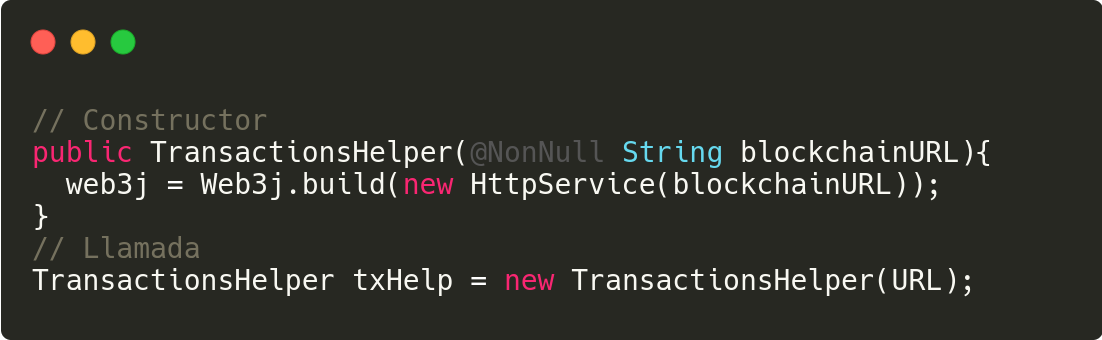
\includegraphics[width=0.8\linewidth]{figs/Desarrollo/SDK/transHelper_constructor}
  \caption[Constructor de TransactionsHelper]{Constructor de TransactionsHelper}
  \label{fig:transH}
\end{figure}

Una vez creado el objeto se puede llamar al resto de funciones, entre las que están \textit{signTransaction(...)} que recibe seis argumentos entre otros las credenciales del wallet, el destino de la transacción (el smart contract) y un \emph{listener} para recuperar la respuesta de la transacción. Recordemos, no se pueden hacer operaciones pesadas en el hilo principal de Android por lo que hay que hacerlo en un hilo a parte (es decir en un \emph{Thread}). Otra función importante es \textit{sendSignedTransaction(...)} la cual recibe dos parámetros, la transacción firmada y un \emph{listener}. Ambas funciones están ``sobrecargadas'' (sobrecarga es la capacidad de un lenguaje de programación, que permite nombrar con el mismo identificador diferentes variables u operaciones), la razón de esta sobrecarga es permitir pasar los parámetro de múltiples maneras. Por ejemplo, los datos de la transacción se pueden pasar como JSON, como String, como HashMap\dots y gracias a la sobrecarga podemos ponerle el mismo nombre a la función. A grandes rasgos un pequeño ejemplo de código puede verse en \ref{fig:firmEnv} y un ejemplo completo de función puede verse en el Anexo \ref{fig:firma_envia_completo}

% \begin{lstlisting}[language=Java,float=ht,caption={[Java] Firmar y Enviar transacciones.},label=lst:transactionHelper]
% // Se crea y firma la transacción
% EthGetTransactionCount ethGetTransactionCount = null;
% ethGetTransactionCount = web3j.ethGetTransactionCount(credentials.getAddress(), DefaultBlockParameterName.LATEST).send();
% BigInteger nonce = ethGetTransactionCount.getTransactionCount();
% RawTransaction rawTransaction = RawTransaction.createTransaction(parametrosJSON);
% byte [] signedTx = TransactionEncoder.signMessage(rawTransaction, credentials)
% signedMessage = Numeric.toHexString(signedTx);
% 
% // Se envía la transacción
% EthSendTransaction ethSendTransaction = web3j.ethSendRawTransaction(signedMessage).send();
% \end{lstlisting}

\begin{figure}[h!]
  \centering
  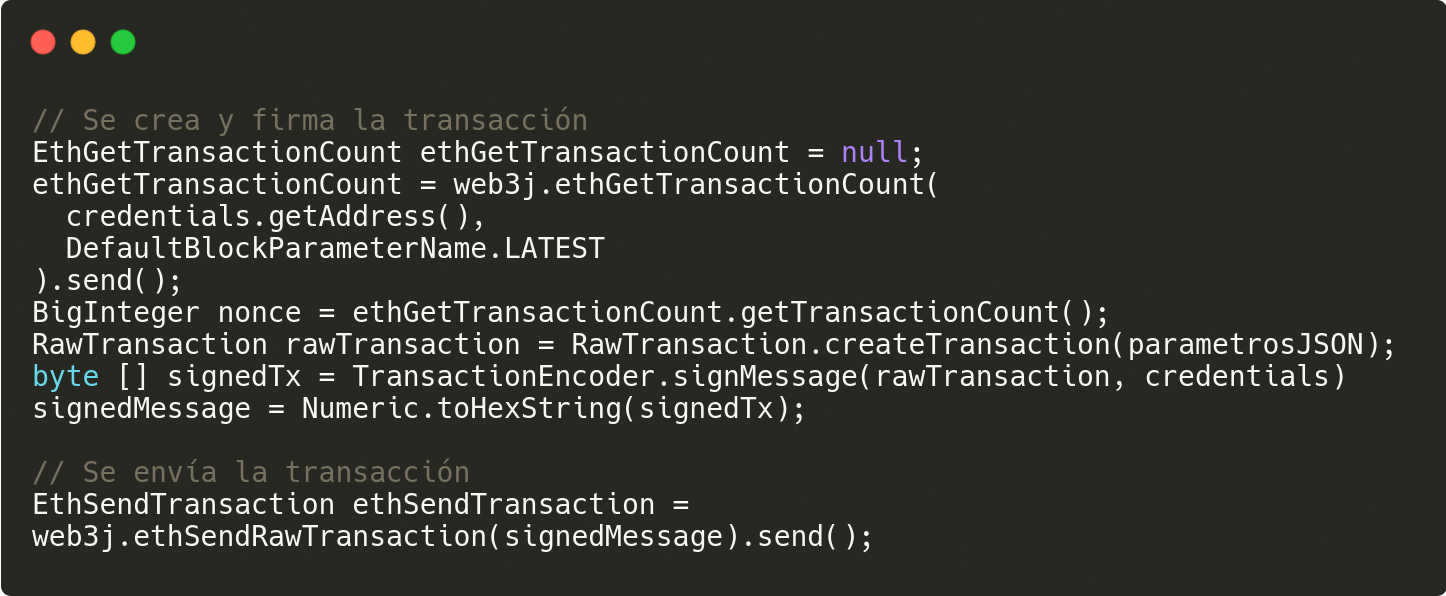
\includegraphics[width=0.8\linewidth]{figs/Desarrollo/SDK/firm_env_trans}
  \caption[Firmado y enviado de una transacción]{Firmado y enviado de una transacción}
  \label{fig:firmEnv}
\end{figure}



% --------------------------------------------------
\subsection{Comunicación con el Dispositivo Móvil}

Para facilitar la generación de credenciales, wallets, guardar en la carpeta ``Shared Preferences'' de Android todos los datos necesarios para la comunicación con la red blockchain\dots Tenemos el archivo \emph{WalletHelper.java}. En él además de la librería web3j, tenemos algunas funcionalidades de Seguridad de Java para modificar el proveedor de seguridad, y permitir que salten errores por algoritmos o parámetros erróneos. \\

En este archivo tenemos entonces un constructor, el cual modifica el proveedor de seguridad a causa de un error con el algoritmo ``Elliptic Curve Digital Signature Algorithm''(ECDSA)\cite{ecdsa} para el proveedor BC\cite{bc}. Más información sobre el error se puede encontrar en el repositorio de web3j en la \href{https://github.com/web3j/web3j/issues/915}{issue\_915}. Básicamente lo que hace el código es modificar el proveedor \ref{fig:ecdsa} \\

% \begin{lstlisting}[language=Java,float=ht,caption={[Java] Modificación de proveedor de seguridad},label=lst:transactionHelper]
% final Provider provider = Security.getProvider(BouncyCastleProvider.PROVIDER_NAME);
% if(provider != null || !provider.getClass().equals(BouncyCastleProvider.class)){
%   Security.removeProvider(BouncyCastleProvider.PROVIDER_NAME);
%   Security.insertProviderAt(new BouncyCastleProvider(), 1);
% }
% \end{lstlisting}

\begin{figure}[h!]
  \centering
  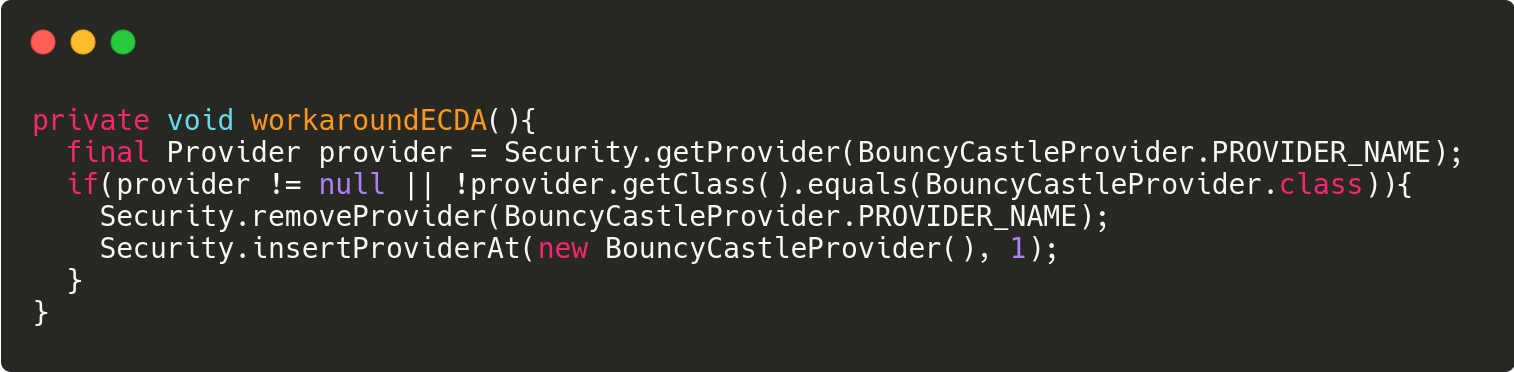
\includegraphics[width=0.8\linewidth]{figs/Desarrollo/SDK/ecdsa}
  \caption[Modificación de proveedor de seguridad]{Modificación de proveedor de seguridad}
  \label{fig:ecdsa}
\end{figure}

Luego, el programador dispone de varias funciones para crear un nuevo wallet con \textit{createNewWallet(...)}\ref{fig:crearWallet} que acepta dos parámetros, siendo estos una contraseña y luego el lugar en el que se quiere guardar el wallet creado. Al igual que antes, esta función esta sobrecargada permitiendo pasar la localización como objeto String o como objeto File. Y permite también recuperar el \emph{address} del usuario o todas las credenciales\ref{fig:recuperarCredenciales}.

% \begin{lstlisting}[language=Java,float=ht,caption={[Java] Creacion de wallet y recuperación del address},label=lst:transactionHelper]
% WalletUtils.generateLightNewWalletFile(password, new File(keyStoreDirectory));
% 
% Credentials credentials = WalletUtils.loadCredentials(password, keyStoreDirectory);
% String address = credentials.getAddress();
% \end{lstlisting}

\begin{figure}[h!]
  \centering
  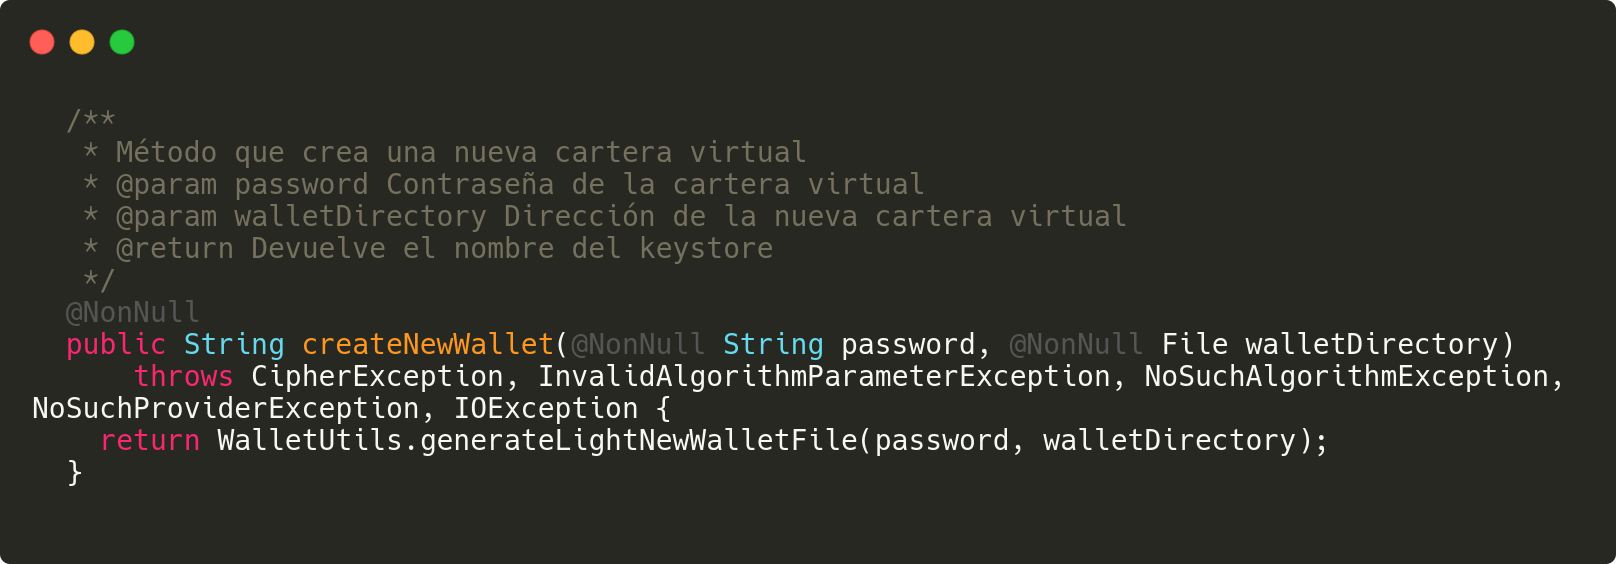
\includegraphics[width=0.8\linewidth]{figs/Desarrollo/SDK/crearWallet}
  \caption[Creación de un nuevo wallet]{Creación de un nuevo wallet}
  \label{fig:crearWallet}
\end{figure}

\begin{figure}[h!]
  \centering
  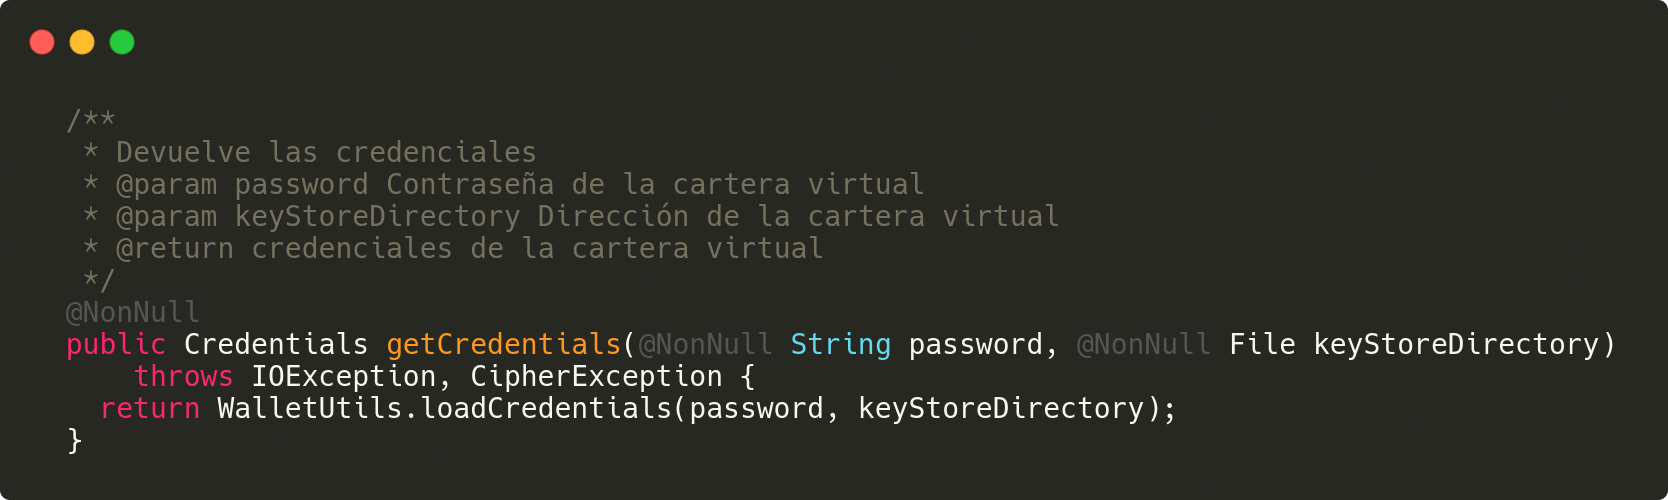
\includegraphics[width=0.8\linewidth]{figs/Desarrollo/SDK/recuperarCredenciales}
  \caption[Recuperación de las credenciales]{Recuperación de las credenciales}
  \label{fig:recuperarCredenciales}
\end{figure}

Como hemos mencionado anteriormente en este archivo se incluye también el guardado de los datos en él dispositivo móvil, aunque la función de web3j \textit{WalletUtils.generateLightNewWalletFile()} guarda los datos en el móvil. Para permitir que un usuario tenga varios wallets, se utiliza el \emph{SharedPreferences} para enlazar al usuario con su wallet. Para ello tenemos la función \textit{saveInPreferences(...)} la cual recibe cuatro parámetros entre ellos el lugar donde guardarlo, y los datos a guardar. Y luego tenemos otro método \textit{getFromPreferences(...)} para recuperar los datos\ref{fig:sharedPref}. \\

% \begin{lstlisting}[language=Java,float=ht,caption={[Java] Guardado y recuperación de dátos en SharedPreferences},label=lst:transactionHelper]
% // Guardamos los datos
% SharedPreferences sharedPreferences = activity.getSharedPreferences(prefsName, Context.MODE_PRIVATE);
% SharedPreferences.Editor editor = sharedPreferences.edit();
% editor.putString(id, walletDirectory);
% editor.apply();
% 
% // Devolvemos el dato con identificador id
% return  sharedPreferences.getString(id, null);
% \end{lstlisting}

\begin{figure}[h!]
  \centering
  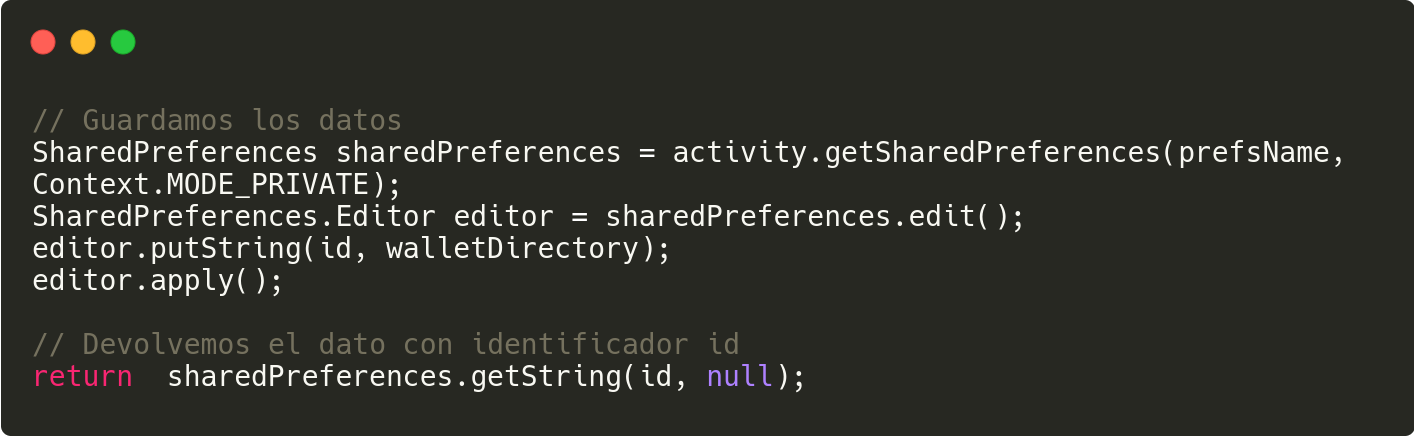
\includegraphics[width=0.8\linewidth]{figs/Desarrollo/SDK/sharedPref}
  \caption[Guardado y recuperación de datos]{Guardado y recuperación de datos}
  \label{fig:sharedPref}
\end{figure}

Se ha decidido utilizar \emph{SharedPreferences} para elegir que wallet desbloquear cuando un usuario hace login, ya que se ha visto la posibilidad de que un mismo usuario necesite más de un wallet. El caso de uso es el siguiente, el presidente de una asociación es alumno y a su vez presidente. Dicho de otro modo, por como esta diseñado ``Estublock'' el usuario tendrá dos wallets, uno para él como estudiante y otro para él como presidente de una asociación. Para ello utilizará por un wallet su correo como alumno y para el otro su correo de asociación, de ahí la necesidad de relacionar el correo con el directorio y nombre del keystore que se genera (más sobre keystore en \hyperref[sec:wallet]{wallet}).

% --------------------------------------------------
\subsection{``Callback Listener''}

Como las llamadas a la red blockchain son pesadas, han sido implementadas con threads: ``\textit{new Threads( new Runnable(){...} )}''. Como el código no espera a la respuesta del thread, se han implementado dos funciones que hacen de ``escucha'' para cuando termina la ejecución. Estas funciones están especificadas en \emph{EasyBlockchainListener.java}, este archivo es una \emph{interdaz de java} para poder ser sobrescritas por le programador para que las funciones hagan lo que el programador desee. Utilizando la anotación de java \textit{@Override} con la que se sobrescribe un método para que el programador cambie el código y pueda hacer con la respuesta lo que considere necesario. Tenemos dos callbacks, uno para cuando se firma la transacción, y otro para cuando se envía a la red blockchain. Para utilizarlos no hay más que pasar como último parámetro de las funciones anteriormente mencionadas una función que será la que sobrescriba a los métodos como se puede ver en \ref{fig:callback}.

% \begin{lstlisting}[language=Java,float=ht,caption={[Java] Ejemplo de sobrescritura de un listener.},label=lst:transactionHelper]
% public void doSomething(...){
%   signTransaction(credentials, gasPrice, gas, to, data, new EasyBlockchainListener() {
%     // Sobrescribimos el método que esta en la interfaz EasyBlockchainListener
%     @Override
%     public void onSignTransactionEvent(@NonNull @NotNull String signedTx) {
%       sendSignedTransaction(signedTx);
%     }
%   });
% }
% \end{lstlisting}

\begin{figure}[h!]
  \centering
  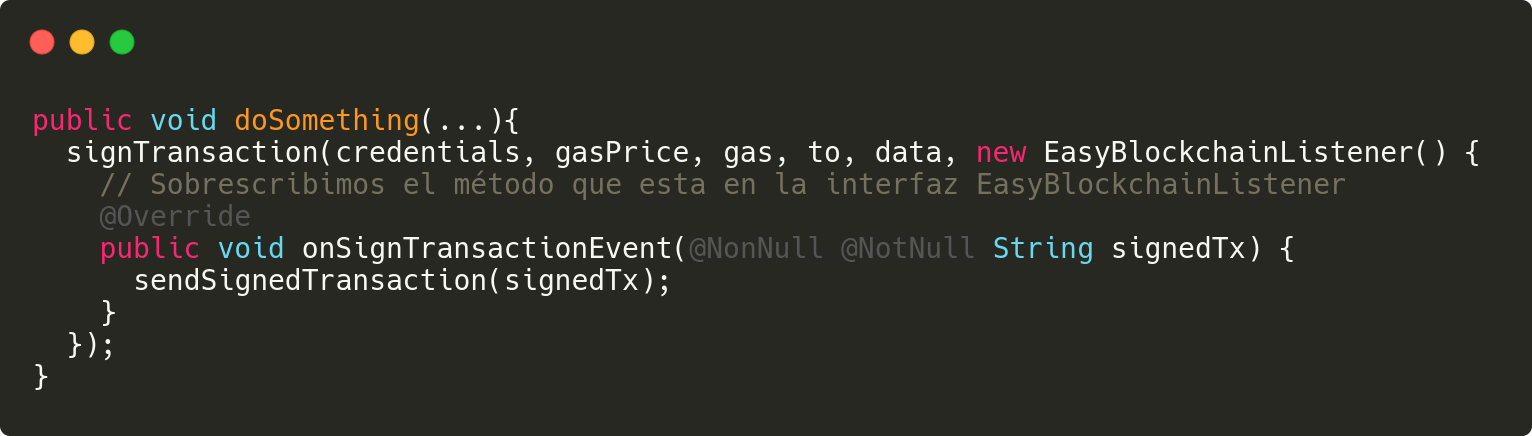
\includegraphics[width=0.8\linewidth]{figs/Desarrollo/SDK/callback}
  \caption[Función de ejemplo de un callback]{Función de ejemplo de un callback}
  \label{fig:callback}
\end{figure}

\subsection{Pruebas del SDK}

Para verificar el correcto funcionamiento del SDK desarrollado, se han realizado varias pruebas. Por un lado tenemos pruebas realizadas directamente con la aplicación en funcionamiento. Es decir, se ejecuta la aplicación, se crea un usuario y se mira si se ha creado correctamente el keystore y si las \emph{Shared Preferences} de Android tienen guardada la relación entre usuario y keystore. También se prueba que al crear un nuevo evento la transacción se firme y se vea reflejada en la red blockchain. Por último, se comprueba que se escanee correctamente el código QR y se vea reflejada la asistencia en la red blockchain, y se verifica también que se genere correctamente el QR con los datos del usuario, en concreto, el address. Estas pruebas, además de verificar que el SDK funciona, también comprueban el correctamente funcionamiento de las librerías al estar haciendo llamadas a las APIs, generando QRs y llamando a la cámara de fótos. \\

Por otro lado, más precisamente para probar llamadas a una red blockchain con más rápidez, se ha utilizado \textbf{ganache}\cite{ganache}. Ganache permite levantar una red blockchain de pruebas creando además 10 cuentas aleatorias para poder ``experimentar'' con ellas. La prueba ha consistido en desplegar un smart contract en la red, y firmar transacciones y enviarlas a la red blockchain de ganache. La ventaja de utilizar ganache es poder utilizar \textbf{Geth} desde la consola de linux para ver información sobre lo que esta sucediendo en la red blcockchain de forma local sin riesgos de comprometer la red blockchain original que se utiliza en ``Estublock''. \textbf{Geth}\cite{geth} es una implementación en el lenguaje \emph{Golang} del protocolo de Ethereum. Lógicamente, el objetivo de estas pruebas al igual que las anteriores era buscar errores, fallos, bugs\dots

% --------------------------------------------------
\subsection{Como Incorporarlo en Otras Aplicaciones} \label{sec:Maven}

Para que otro programador pueda utilizar el SDK que se ha desarrollado el primer paso es publicar el SDK en algún repositorio como en los repositorios de \emph{Maven Centra}\cite{maven}. Maven dispone de una inmensa cantidad de repositorios que usuarios pueden utilizar añadiendo la dependencia a sus proyectos, y gradle (el sistema de automatización de construcción de código que utiliza Android) se encarga de bajar la información automáticamente y así el usuario puede utilizar las funcionalidades que el usuario desea. Esta comodidad y facilidad en la gestión del SDK es la razón por la que se ha decidido utilizar \emph{Maven}. Una alternativa era utilizar \emph{jcenter()} sin embargo, no se ha hecho puesto que la empresa que mantiene el repositorio JCenter (empresa llamada \emph{JFrog}\cite{jfrog}) lo convirtió en un repositorio de solo lectura el \textbf{31 de Marzo de 2021}. \\

Para publicar la librería se han de seguir a muy grandes rasgos estos pasos:
\begin{itemize}
\item Crear un ``ticket'' con \emph{Sonatype}\cite{sonatype}.
\item Crear el proyecto en Sonatype.
\item Verificación de propiedad mediante DNS.
\item Instalación del plugin para gradle \href{https://github.com/vanniktech/gradle-maven-publish-plugin}{gradle-maven-publish-plugin}
\item Generar llaves GPG
\item Configurar firmas
\item Subir los artifacts a Sonatype
\item Publicar la librería
\end{itemize}

Más detalles se pueden encontrar en el post de ``Waseef Akhtar''\cite{waseef}. \\

Una vez la librería es pública, cualquier programador puede añadirla a su proyecto añadiendo a sus dependencias la línea \textit{implementation 'com.<entidad>.estublock:EasyBlockchain:1.0.0'}, el nombre de la entidad aún está por definir. Una vez añadida la línea y después de que gradle termine de sincronizar el repositorio, el programador puede utilizar todas las funciones que hayan en la versión 1.0.0 del SDK.


\section{Wallet} \label{sec:wallet}

El wallet es una aplicación que permite interactuar con la cuenta de Ethereum. Puede verse como una aplicación bancaria, que te permite ver tu saldo, enviar transacciones y conectar con aplicaciones. En el caso de ``Estublock'' no existe el concepto de saldo, pero sí se hacen transacciones y llamadas a una aplicación (el smart contract que tenemos ejecutando en la red blockchain a la que hacemos llamadas). El wallet guarda las credenciales del usuario, también conocidas como \textbf{keystore}. \\

Cuando en la aplicación se registra un nuevo usuario, se le crea un wallet y se guarda este wallet con las credenciales en el dispositivo móvil. En el keystore se guarda la clave privada del usuario. Una clave privada en Ethereum no es más que 64 caracteres hexadecimales elegidos al azar. Aunque cualquiera pudiera elegir la clave privada manualmente, no es recomendable por seguridad. La clave pública se deriva de la clave privada utilizando el algoritmo de curva elíptica ECDSA \emph{Elliptic Curve Digital Signature Algorithm}. Una vez se tiene la clave pública y privada, se recupera el address del usuario, con este address se identifica al usuario en la red blockchain. En Ethereum se coge la clave pública y se ejecuta la función hash ``\emph{SHA 3}'' sobre ella, y como resultado se obtienen 64 caracteres de los cuales los últimos 40 son el address del usuario. Lógicamente todo este proceso lo hace la aplicación ``Estublock'' con ayuda del SDK y de la librería \emph{web3j}. \\

Para añadir una capa de seguridad al keystore, y la clave privada quede cifrada, se añade una contraseña de cifrado que el usuario debe introducir para desbloquear el wallet. En la aplicación se ha decidido que la contraseña que se va a utilizar para desbloquear el wallet sea la misma que la que se utiliza para hacer login. Por lo tanto, una vez hecho el login, el usuario no debe introducir la contraseña nuevamente para hacer las transacciones. La clave \textbf{privada} se utiliza para firmar las transacciones que se envían a la red blockchain, y la clave \textbf{pública} se utiliza para que cualquier persona pueda verificar la firma. \\

% ----------------------------------
\subsection{Gestión del Wallet}

Existen distintos tipos de wallet\ref{fig:tipos_wallet}. Cada uno con sus ventajas y desventajas. Los ``web wallet'', son los más fáciles de utilizar, pero traen consigo un incoveniente. El usuario no tiene el control de sus credenciales. Las credenciales del usuario las mantiene una empresa externa. Por eso no se ha pensado en este tipo de wallets para la aplicación. Por otro lado tenemos las ``Cold Wallets'', las cuales son muy seguras, y el usuario tiene total acceso y control de las credenciales almacenadas en un dispositivo externo sin conexión a internet. La falta de conexión a internet y la incomodidad al usar una cold wallets, fueron la razón por las que se descartó este tipo de wallets para el proyecto. Luego están las dos mejores, \textbf{Hardware y Software Wallets}. Ambas aportan gran seguridad y control de las credenciales, por su usabilidad, las hardware wallets son más incómodas pues se suelen utilizar dispositivos externos para guardar las credenciales, como un disco duro cifrado. Por lo que, la mejor decisión era utilizar las \textbf{Software Wallets} para el proyecto. \\

\begin{figure}[h!]
  \centering
  % https://www.bitpanda.com/academy/en/lessons/what-is-a-wallet-and-how-do-i-get-one/
  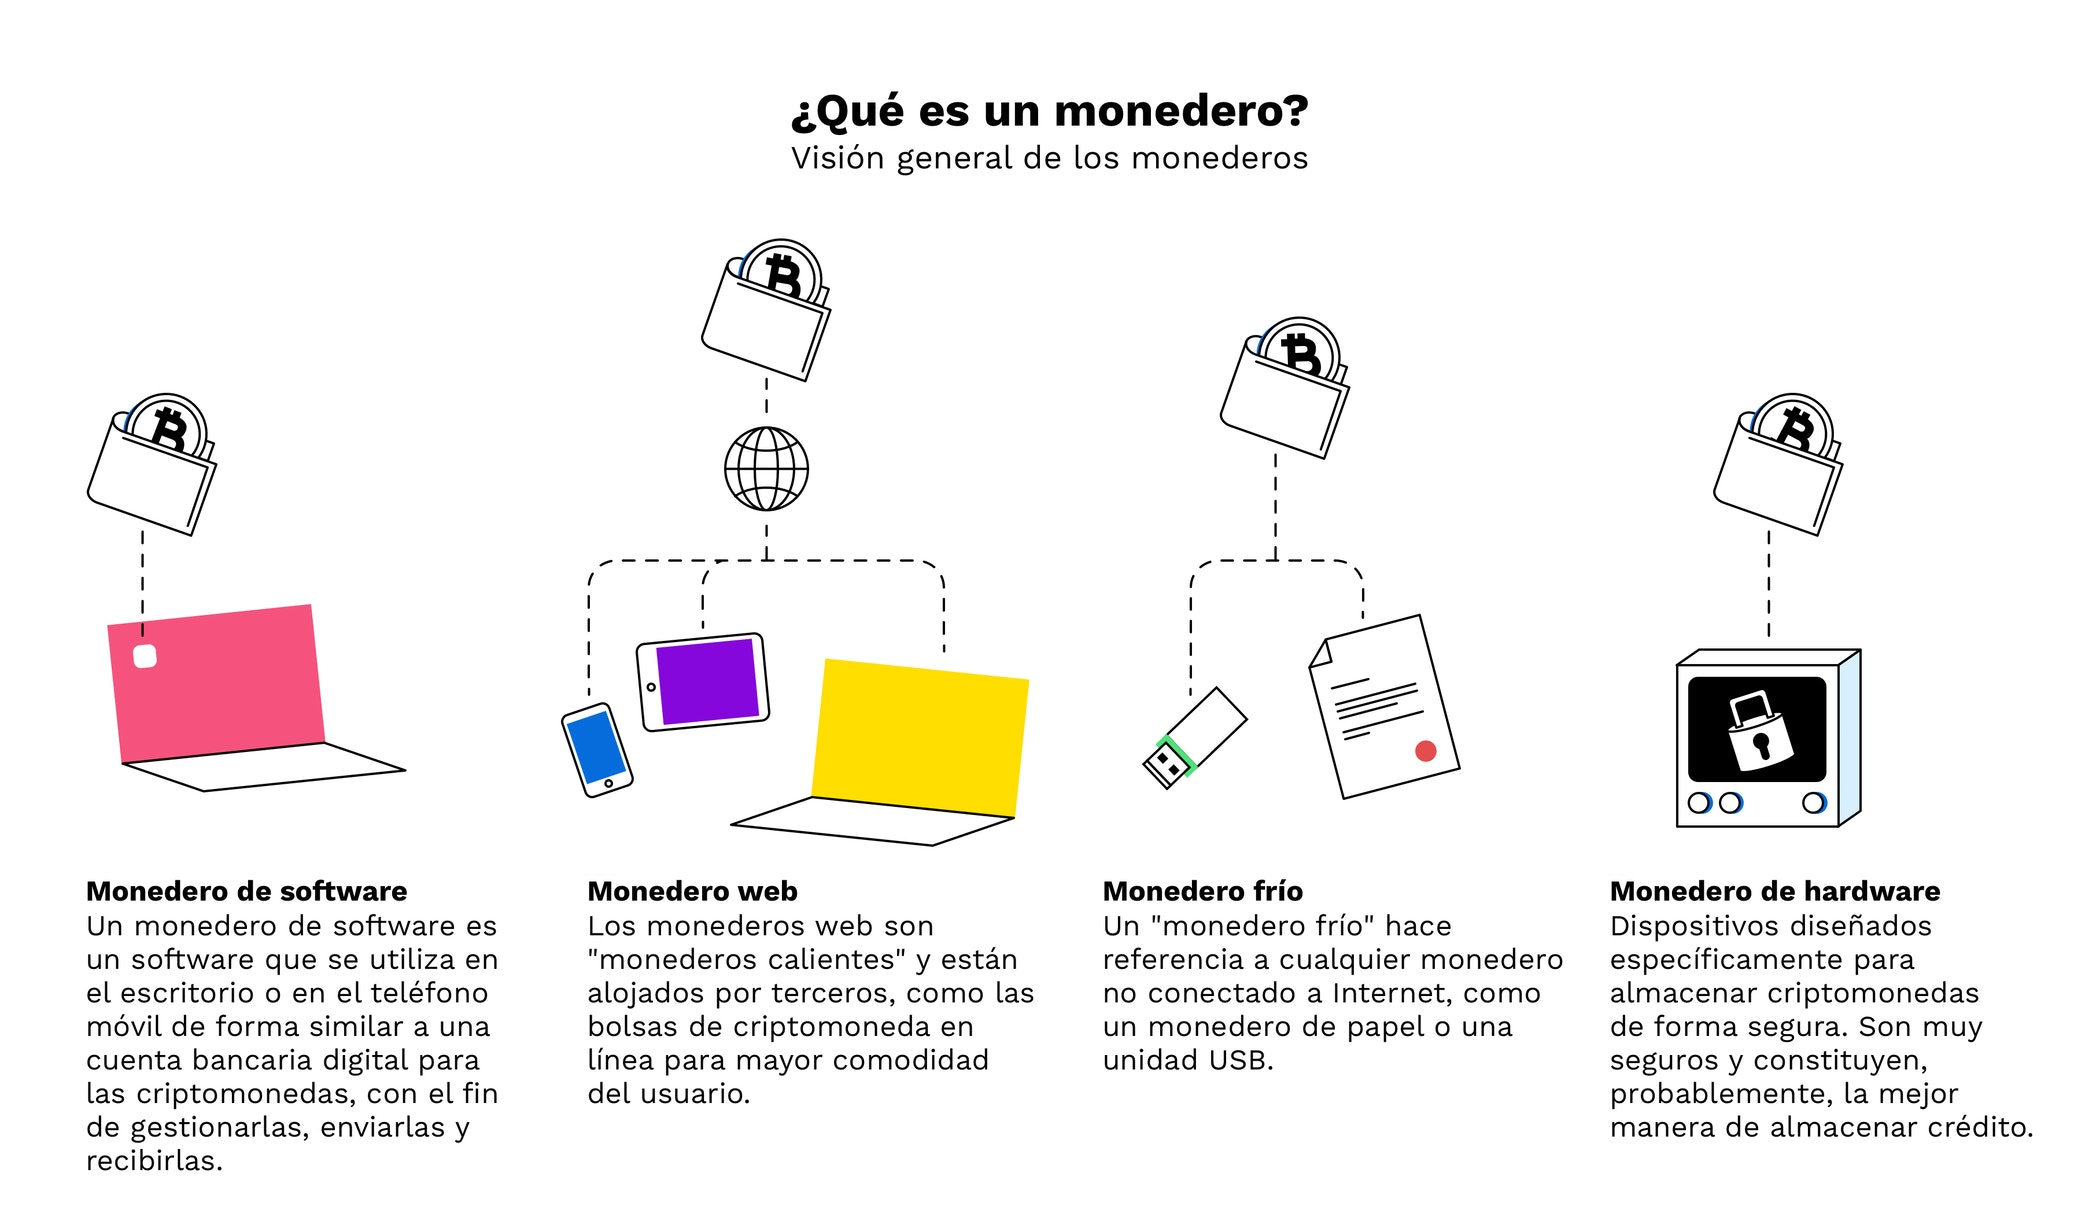
\includegraphics[width=0.8\linewidth]{figs/Desarrollo/Wallet/que_es_wallet}
  \caption[Visión general de los wallets]{Visión general de los wallets}
  \label{fig:tipos_wallet}
\end{figure}

Las software wallets son fáciles de crear, el usuario tiene buen control de las credenciales pues están guardadas en su dispositivo móvil y tiene buena seguridad. Sin embargo hay que destacar las desventajas. Aunque no ocurre de forma habitual, el usuario puede perder el móvil, se lo pueden robar, romper o puede cambiarlo por uno mejor. Todas estas situaciones llevan al mismo lugar, el usuario no tiene acceso al wallet que tenía en el móvil original, y necesita acceso nuevamente al wallet. Otra situación en la que llegamos al mismo problema es \textbf{olvidar} la contraseña que utilizamos para desbloquear el Wallet. \\

\subsection{Perdida y Recuperación del Wallet}

Un usuario puede perder acceso a su wallet a causa de múltiples razones como hemos mencionado antes. Aunque es muy difícil recuperar el acceso al wallet de un usuario, es posible. Existen compañías como el equipo de \emph{walletrecovery}\cite{walletRec} los cuales se encargan de intentar recuperar en la medida de lo posible el acceso a tu wallet. Ya sea por causas hardware o que se ha olvidado la contraseña, probarán métodos de fuerza bruta, programas de recuperación de archivos dañados\dots. No es la única empresa que se encarga de esto, en \emph{WRS}\cite{WRS} también se encargan de recuperar wallets. Por último también existen programas de código abierto los cuales el usuario puede utilizar para recuperar las credenciales en la medida de los posible, programas como \textbf{btcrecover}\cite{btcrecover}. La herramienta permite generar un diccionario de fuerza bruta a partir de información dada por el usuario, así como probar varias combinaciones de palabras dada una ``seed phrase''. \\

En el caso de ``Estublock'' no hay implementado en el presente un sistema de recuperación del wallet. Sin embargo, se pueden implementar tres métodos para evitar que el usuario pierda acceso a dicho wallet. Por un lado tenemos las \textbf{seed phrases}, estas son un conjunto de palabras aleatorias que el usuario debe guardar a buen recaudo y ``bajo llave'' pues pueden servirle en caso de emergencia para recuperar el acceso al wallet. Si el usuario olvida la contraseña, las \emph{seed phrases} servirán para recuperar dicho acceso. Por otro lado, existe la opción de compartir parte de la clave privada con varios usuarios de mucha confianza. En el caso de olvidar la contraseña de su wallet, el usuario tiene acceso a su clave privada reuninedo dicha clave con ayuda de esas personas de mucha confianza. Una vez reconstruida la clave privada, puede utilizar una nueva contraseña para cifrarla y seguir utilizando sin problemas el sistema. Por último, es ideal que el usuario haga una copia de seguridad del wallet para evitar que perder el móvil, o fallos en el móvil (archivos corruptos, móvil roto\dots) o un robo puedan hacerle perder el acceso al wallet. 

% ##################################################
% ##################################################
\section{Documentación}

La documentación es tan importante como la implementación, hay debate sobre si la documentación es una obligación o una recomendación muy positiva. La experiencia desarrollando, nos ha demostrado que una buena documentación es clave para que un programa pueda seguir siendo desarrollado, entendido, mantenido, y sirva a otros desarrolladores. Una buena documentación garantiza un producto final de mayor calidad. Aunque no hay un método estricto en cuanto ha ``cuándo hay que poner comentarios'', se ha decidido poner comentarios al inicio de la clase, de los métodos y de las variables de clase. Así como en fragmentos de código no evidentes y en los que se hace algo raro. \\

Aunque la documentación dentro del código es un método correcto de documentar, un programador no tiende a mirar el código fuente, sino una documentación externa. Existen múltiples métodos para documentar y generar documentación, \textbf{Read the Docs}\cite{readthedocs} por ejemplo simplifica el proceso de documentación automatizando la construcción, versionado y ``hosting'' de la documentación de tus programas. Es gratis, siempre actualizado y permite descargar la documentación en varios formatos, así como mostrar documentación de varias versiones del proyecto. Por otro lado tenemos \textbf{JavaDocs}\cite{javadocs} es el formato por defecto para todo proyecto Java, permite generar una página web con la documentación que hay en los comentarios que hay en el programa. También es gratis pero no tiene opción de ``hosting'', es el programador el que debe dar el servicio online o que cada programador se genere la documentación en local. Por otro lado, para el futuro de la apliación, en el caso de que se migre el código a \emph{Kotlin} tenemos \textbf{Dokka}\cite{dokka}, permite generar documentación de la misma forma que \emph{javadocs} pero para Kotlin. Por último otra opción es \textbf{Doxygen}\cite{doxygen} es una herramienta de generación de documentación al igual que las anteriormente mencionadas, para lenguajes como \emph{C, C++, Java, PHP, Python}\dots\\

Para documentar el SDK se ha decidido utilizar \textbf{javadocs} pues es muy fácil de utilizar, es fácil documentar el código con la sintaxis de javadocs, y cualquier persona puede generar la documentación o mirar el código fuente para saber que hace cada función, que parámetros se esperan y que datos devuelve. La documentación del código se puede encontrar en el Anexo \ref{fig:docsTransHelper}


\chapter{Análisis de Impacto}
\label{cap:ImpactoMedioAmbiente}

En 2015, la ONU aprobó la \emph{Agenda 2030 sobre el Desarrollo Sostenible}\cite{agenda2030}, una oportunidad para que los países y sus sociedades evolucionen y mejoren la vida de todos, sin dejar a nadie atrás. Constituye un llamamiento universal a la acción para poner fin a la pobreza, proteger el planeta y mejorar la vida de personas y animales. Se aprobaron entonces 17 objetivos\cite{17objetivos} a alcanzar en 15 años. \\

Dentro de los 17 objetivos, hay 2 muy importantes en los que la aplicación Estublock juega un papel. La tecnología blockchain aporta sin duda una gran cantidad de ventajas, como la fiabilidad, transparencia de las operaciones (el código de los smart contracts esta a disposición de la gente), seguridad de los datos, inmutabilidad, anonimato\dots Pero, estas ventajas traen consigo una pequeña desventaja a nivel medioambiental. Como sabemos, una red blockchain es \emph{descentralizada}, esto se debe a que hay varios nodos conectados entre si. Cada nodo es un ordenador en constante ejecución lo que repercute en el consumo de electricidad. Esto multiplicado por cada ordenador que hay en la red blockchain. Por ejemplo, la red de bitcoin dispone a día de hoy \textit{2021-05-24} de 9786 nodos\cite{bitcoinNodos} lo cuales consumen bastante energía\ref{fig:electricidad_bitcoin}. \\

\begin{figure}[h!]
  \centering
  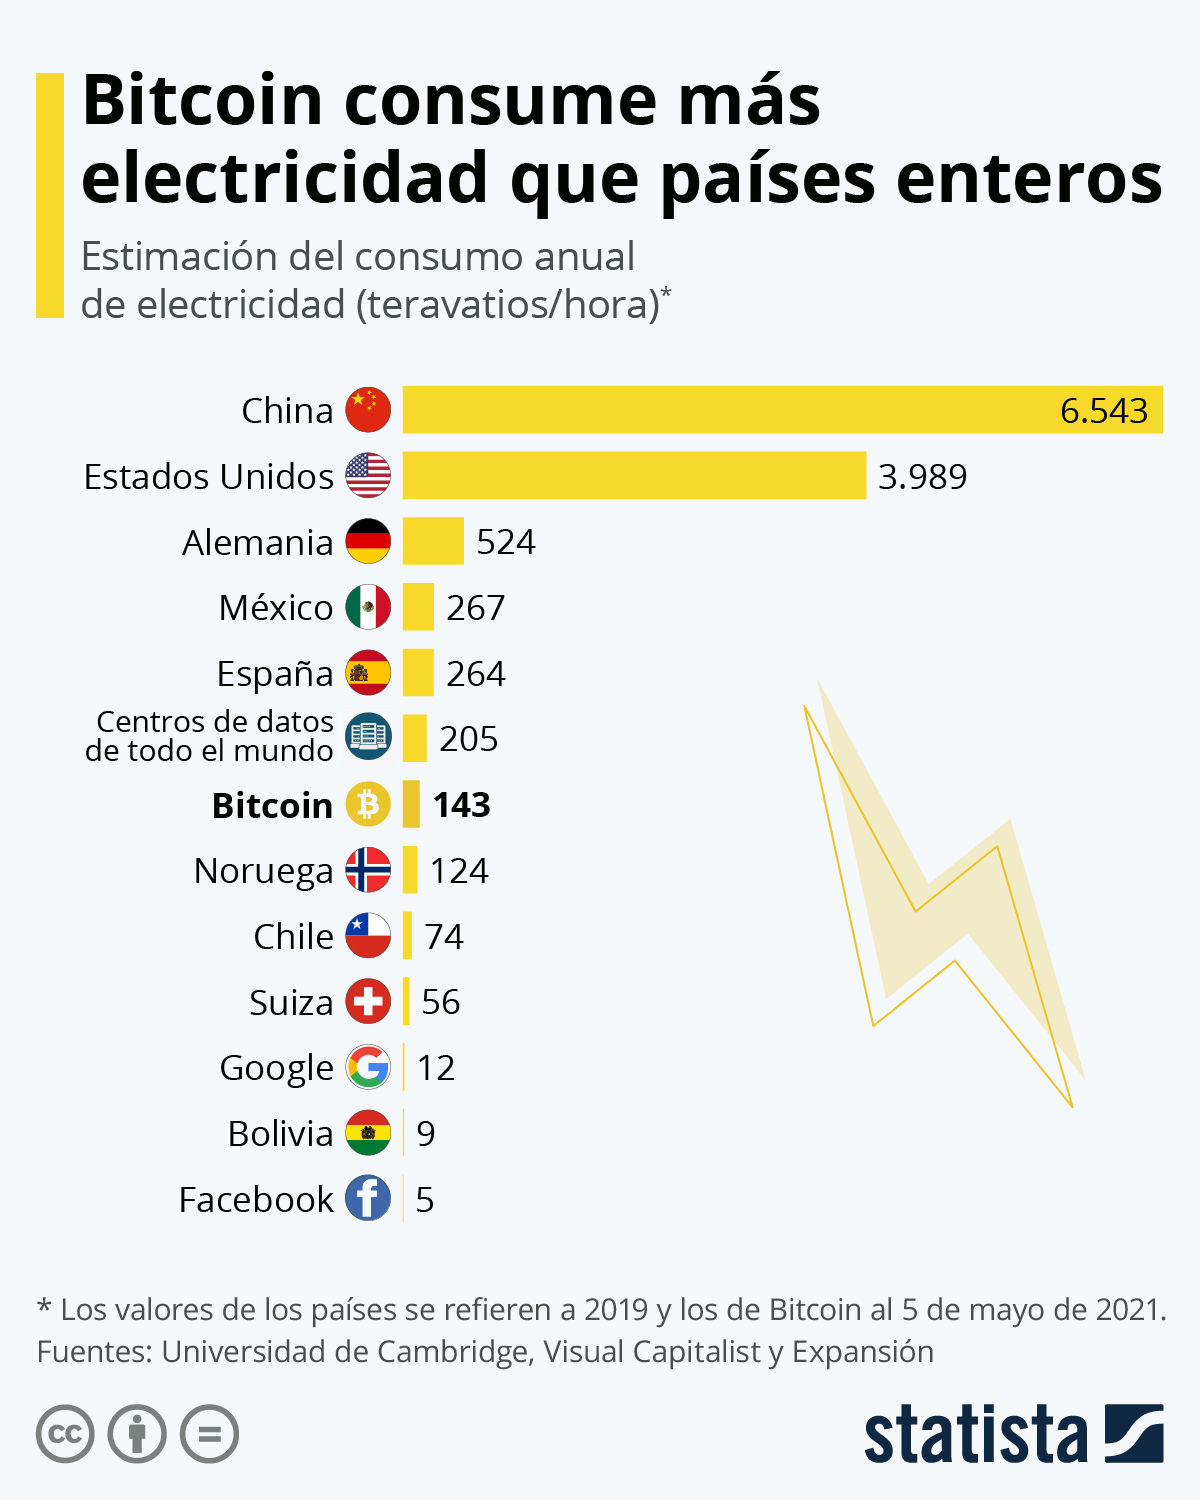
\includegraphics[width=1\linewidth]{figs/ImpactoMedioAmbiente/electricidad_bitcoin}
  \caption[Consumo eléctrico de bitcoin]{Consumo eléctrico de bitcoin}
  \label{fig:electricidad_bitcoin}
\end{figure}

Por suerte, aunque parezca que blockchain va a consumir tanta energía como el \textit{Centro de Datos de Todo el Mundo}, en 2019 \emph{Coinshares} realizó una investigación\cite{coinshare} que reveló que el 74\% de las operaciones mineras se realizan con energía renovable, por lo que el impacto medioambiental es menos grave de lo que podría ser. Sin embargo, siempre se puede mejorar, y llegar al 100\% de consumo con energías renovables. \emph{Ethereum versión 2}\cite{Ethereum2.0} es la alternativa verde a este problema, al cambiar el algoritmo de consenso de \textit{Proof of Work} a \textit{Proof of Stake}, ethereum disminuirá casi completamente el consumo de energía. Hasta tal punto, de que \textbf{Joseph Pallant}, fundador de la \emph{blockchain for climate foundation}\cite{bkClimateF} (una fundación que busca utilizar la tecnología blockchain para lidiar con problemas relaciodos con el cambio climático) utiliza Ethereum2.0. Aunque esta segunda versión de Ethereum ya esta en funcionamiento, se requiere de un tiempo para migrar los datos de la versión 1 a la 2, pero con el tiempo la versión 2 de ethereum crecerá, disminuyendo enormemente el gasto energético que conlleva. \\

Aunque Estublock utiliza actualmente la red de Ethereum1.0, su gasto energético es de todos modos casi nulo (pues no hay suficiente tráfico como para que suponga un gasto energético grande), pero hay que tener en cuenta que aunque la red gaste poco, hay varios ordenadores encendidos consumiendo energía, por lo que habrá que migrar a Ethereum2.0 cuando sea posible. Aunque el gasto energético es muy bajo, no se debe olvidar que gastar energía, gasta y que sería recomendable lograr que los ordenadores estén lo más especializados posible para minimizar al máximo el gasto energético cumpliendo con el objetivo \textit{9.4} ``modernizar la infraestructura para que sean sostenibles''. ``Estublock'' tiene también un impacto en el punto \textbf{13} ``Acción por el Clima'' con respecto al objetivo de minimizar las emisiones de carbono al máximo, en las universidades en las que se utilice la aplicación ``Estublock'' y dispongan de nodos en la red blockchain, se puede tratar de utilizar siempre energías renovables como poner paneles solares en la universidad para que los nodos de la red utilicen esa energía renovable para funcionar.


\chapter{Conclusiones}
\label{cap:Conclusiones}

En este capítulo se realizará un juicio crítico y discusión sobre los resultados obtenidos. \emph{Cuidado, esta discusión no debe confundirse con una valoración del enriquecimiento personal que supone la realización del trabajo como culminación de una etapa académica}. Aunque de gran importancia, esta última valoración debe quedar fuera de la memoria del trabajo y solo debe ahondarse en ella ante requerimiento explícito del comité en el acto de defensa.

Si es pertinente deberá incluir información sobre trabajos derivados como publicaciones o ponencias en preparación, así como trabajos futuros \emph{(solo si estos están iniciados o planificados en el momento que se redacta el texto)}. Evitar hacer una lista de posibles mejoras. Contrariamente a lo que alguno pueda pensar generalmente aportan impresión de trabajo incompleto o inacabado.\footnote{Puede reflexionarse en ello por si en la defensa del trabajo se pregunta sobre estas posibles mejoras.}


\section{Justificación de competencias adquiridas}
Es muy importante recordar que según la normativa vigente, el capítulo de conclusiones debe incluir \emph{obligatoriamente} un apartado destinado a justificar la aplicación en el TFG de competencias específicas (dos o más) asociadas a la tecnología específica cursada.\index{competencias@\textbf{competencias}}

En el TFG se han trabajado las competencias correspondientes a la Tecnología Específica de \emph{[poner lo que corresponda]}:

\begin{description}
\item[Código de la competencia 1:] \emph{[Texto de la competencia 1]}. Explicación de cómo dicha competencia se ha trabajado en el TFG.
\item[Código de la competencia 2:] \emph{[Texto de la competencia 2]}. Explicación de cómo dicha competencia se ha trabajado en el TFG.
\end{description}

\dots otras más si las hubiera.


\section{Planificación y costes}
En este capítulo se puede incluir una valoración del trabajo realizado en el que se justifique el tiempo dedicado al TFG teniendo en cuenta que este tiene asignados 12 créditos ECTS\index{ECTS} que se traducen en {300-360} horas totales. En este sentido una correcta planificación del TFG debería garantizar que el trabajo se realice dentro de la horquilla señalada. Queda a criterio del tribunal la evaluación de valores extremos por defecto o exceso en función de los resultados obtenidos.

Es muy importante que todas las justificaciones aportadas se sustenten no solo en juicios de valor sino en evidencias tangibles como: historiales de actividad, repositorios de código y documentación, porciones de código, trazas de ejecución, capturas de pantalla, demos, etc.




\chapter{Trabajo Futuro}
\label{cap:Futuro}

Actualmente la aplicación ``Estublock'' puede utilizarse para registrar las asistencias a eventos en una universidad sin problema. Sin embargo es largo el camino que le queda para poder decir que esta terminada y que se pueda lanzar la primera versión de la aplicación. Ahora mismo es lo que se conoce como ``una versión alpha''. Esta listo para ser probado pero no para que se utilice de forma masiva. ¿Que avances y siguientes pasos necesita la aplicación para poder lanzar la primera versión \emph{V.1.0.0}? \\

Actualmente el código es ligeramente caótico, durante los meses de desarrollo ha ido sufriendo muchos cambios, renombrado de archivos, creación y eliminación de código y archivos que en su momento tenían utilidad pero ya no. Y todo esto causa que tanto código como archivos, no estén tan ordenados y organizados como deberían. Lo ideal es entonces ordenarlo en carpetas con nombres significativos y eliminando toda repetición de código así como archivos que no hagan falta o crear archivos que pueden hacer que el código sea más mantenible. Esto es fundamental, pues para un futuro programador es más fácil coger un proyecto ordenado y estructurado siguiendo un ``modus operandi'', a coger un proyecto caótico. Además, ordenar el código reduce errores al minimizar las líneas de código (por quitar código repetido) y permite tener mayor control de las funciones que causan problemas. \\
 
Como toda pieza de software, se necesitan tests para probar el correcto funcionamiento de la aplicación. Con una buena batería de tests, el programador puede probar el código que escribe, reduciendo los errores y reduciendo el tiempo que se tarda en corregirlos. Esto se debe a que los errores se detectan con más antelación y de forma más concreta. Dando lugar a un código mas estable, escalable y sostenible en el tiempo. Como no se disponía de experiencia en el desarrollo de aplicaciones móvil, ha sido difícil crear tests unitarios pues el código sufría muchos cambios diariamente con muchas modificaciones en el nombre de variables. Ahora que el código es más estable, y se tiene más experiencia, es un buen momento para desarrollar estos tests unitarios. \\

La documentación es también uno de los pilares de un buen software. Actualmente las funciones tienen pequeños comentarios, excepto las del SDK que están completamente comentadas. Sería ideal añadir comentarios completos en el resto de funciones siguiendo el estilo de comentarios de javadocs para poder generar posteriormente con esta herramienta una documentación más detallada. Muchas partes del código se explican por si mismas, pero la documentación es fundamental para que un proyecto sea mantenido en el tiempo, principalmente para que los futuros desarrolladores entiendan el código ya existente y no pierdan tiempo en averiguar que es lo que hace el código. \\

Con respecto a la interfaz de usuario, esta se ha mantenido muy sencilla. Pero una mejora en el diseño o un remodelado visual pueden hacer que la aplicación sea mucho más atractiva, haciendo que los usuarios disfruten mucho más con su uso. Así como, mejorar la experiencia de los usuarios al utilizarla. Para ello, se puede por ejemplo añadir una opción que permita al usuario personalizar a su gusto el tema de la aplicación, o alguna pantalla o botón que quieran poder mover de sitio. \\

Como se ha mencionado antes, la aplicación permite actualmente registrar las asistencias a eventos, así como crear nuevos eventos, aunque estas sean sus funcionalidades principales, se puede explotar la aplicación mucho más añadiendo nuevas funcionalidades como permitir modificar los datos personales a los usuarios, listar los eventos a los que se ha asistido a lo largo del tiempo o ver los usuarios que han asistido a un evento concreto. También, muy importante, ha de hacerse la diferencia entre alumno y profesor, mostrando distintas pantallas y funcionalidades según el usuario sea un profesor o un alumno. \\

Por último, si miramos más en el futuro. Uno de los objetivos estrella del proyecto ``Estublock'' es llegar a todos los campus de la Universidad Politécnica de Madrid, y posteriormente, al resto de universidades de Madrid y España. Aunque sea un objetivo muy lejano, no hay olvidarlo, este proyecto puede tener un impacto muy positivo en las universidades. Por ello, aunque sea lejano, hay que tener en mente que queremos llegar a todo el mundo. 

% -------------------------

% No olvides retornar al interlineado sencillo en el resto del documento.
\singlespacing

%--- BACKMATTER
%\backmatter (se comenta para que los apéndices puedan aparecer después de la bibliografía)


% -------------------------
%
%--- BIBLIOGRAFÍA
%
% -------------------------
% BEGIN_FOLD
\cleardoublepage % Necesario para ajustar el avance de página
\phantomsection  % Ojo necesario con hyperref.
\addcontentsline{toc}{chapter}{\bibname} % Añade la bibliografía al Índice de contenidos. Se debe mantaner cuando se desean subbibliografías.
%---
% Opción 1: Bibliografía con todas las fuentes en un apartado.
%---
\printbibliography
%---

%---
% Opción 2: Bibliografía con secciones separadas.
%---
%\printbibheading
% Se puede incluir un apartado de fuentes de consulta no citadas
% Como no están citadas es preciso incluir comando \nocite{<key>}
% Se añaden palabras clave a las entradas en el fichero *.bib para poder diferenciarlas
%\printbibliography[heading=subbibliography,keyword=consulta,title={Fuentes de consulta}]
%\printbibliography[heading=subbibliography,keyword=url,title={Direcciones de Internet}]
% -------------------------
% END_FOLD



% -------------------------
%
%--- ANEXOS: Comentar si no se desean incluir. [OPT.]
% Mover si se desea que aparezcan antes de la bobliografía.
%
% -------------------------
%BEGIN_FOLD
% \appendix
% \portadaAnexos % OPT. Añade una portada para anexos

% Tras este punto los capítulos se numeran con letras.
% Aquí todos los apéndices necesarios
\chapter{Anexo}
\label{cap:Anexo}

\begin{figure}[h!]
  \centering
  \includegraphics[width=1\linewidth]{figs/Anexo/zxing}
  \caption[Código del escaneado de QRs]{Código del escaneado de QRs}
  \label{fig:escaneandoQRs}
\end{figure}

\begin{figure}[h!]
  \centering
  \includegraphics[width=1\linewidth]{figs/Anexo/gs}
  \caption[Código de GlobalState]{Código de GlobalState}
  \label{fig:gs}
\end{figure}


 % Apéndice A (opcionales)

%---








% -------------------------
%
% OPT.: ÍNDICE TEMÁTICO: Comentar si no se desean incluir.
%
% -------------------------
% CONSEJO: Incluir los comandos mientras se escribe cada capítulo ya que hacerlo al final resulta tedioso.
%\cleardoublepage % Necesario para ajustar el avance de página
%\phantomsection  % Ojo necesario con hyperref.
%% Permite cambiar el nombre del índice temático
%%\renewcommand{\indexname}{Título del índice}
%\addcontentsline{toc}{chapter}{\indexname} % Añade al Índice de contenidos.
%\printindex  % Facilitado por makeidx (opcional, si no se usa no se imprime)
%---
%END_FOLD
\end{document}
